\documentclass[
	a4paper, % Page size
	fontsize=12pt, % Base font size
	twoside=true, % Use different layouts for even and odd pages (in particular, if twoside=true, the margin column will be always on the outside)
    open=right, % If twoside=true, uncomment this to force new chapters to start on any page, not only on right (odd) pages
	%chapterentrydots=true, % Uncomment to output dots from the chapter name to the page number in the table of contents
	numbers=noenddot, % Comment to output dots after chapter numbers; the most common values for this option are: enddot, noenddot and auto (see the KOMAScript documentation for an in-depth explanation)
]{kaobook}

\usepackage{tikz}
\usetikzlibrary{decorations.pathreplacing, calc, positioning, backgrounds}
\usepackage{svg}

% Custom commands
\newcommand{\der}[2]{\frac{\partial #1}{\partial #2}}
\newcommand{\std}[1]{$\pm$ #1}
\newcommand{\result}[2]{#1$_{\pm #2}$}


% Provides subfigure environment
\usepackage{subcaption}

% Choose the language
\ifxetexorluatex
	\usepackage{polyglossia}
	\setmainlanguage{english}
\else
	\usepackage[english]{babel} % Load characters and hyphenation
\fi
\usepackage[english=british]{csquotes}	% English quotes

% Load packages for testing
\usepackage{blindtext}
%\usepackage{showframe} % Uncomment to show boxes around the text area, margin, header and footer
%\usepackage{showlabels} % Uncomment to output the content of \label commands to the document where they are used

% Load the bibliography package
\usepackage{kaobiblio}
\addbibresource{main.bib} % Bibliography file

% Load mathematical packages for theorems and related environments
\usepackage[framed=true]{kaotheorems}

% Load the package for hyperreferences
\usepackage{kaorefs}

\graphicspath{{images/}} % Paths in which to look for images

% \makeindex[columns=3, title=Alphabetical Index, intoc] % Make LaTeX produce the files required to compile the index

% \makeglossaries % Make LaTeX produce the files required to compile the glossary
% % \newglossaryentry{Neural Network}{
% 	name=computer,
% 	description={is a programmable machine that receives input, stores and manipulates data, and provides output in a useful format}
% }

% Glossary entries (used in text with e.g. \acrfull{fpsLabel} or \acrshort{fpsLabel})
\newacronym[longplural={States of The Art}]{sotaLabel}{SOTA}{State of The Art}
\newacronym[longplural={Convolutional Neural Networks}]{cnnLabel}{CNN}{Convolutional Neural Network}
\newacronym[longplural={Regions of Interest}]{cnnLabel}{ROI}{Region of Interest}
\newacronym[longplural={Regions of Interest}]{cnnLabel}{ROI}{Region of Interest}

 % Include the glossary definitions

% \makenomenclature % Make LaTeX produce the files required to compile the nomenclature

% Reset sidenote counter at chapters
%\counterwithin*{sidenote}{chapter}

%----------------------------------------------------------------------------------------

\begin{document}

%----------------------------------------------------------------------------------------
%	BOOK INFORMATION
%----------------------------------------------------------------------------------------

\title{Integrating Anatomical Information in Weakly Contrastive Learning for\\Neuroimaging}

\subtitle{Master Thesis in Computer Science}
\subsubtitle{Artificial Intelligence and Information Processing Systems}
\author{Matteo Brunello}
\university{University of Turin}
\department{Computer Science Department}
\supervisor{Marco Grangetto}
\cosupervisor{Carlo Alberto Barbano}
\academicyear{2023-2024}

%----------------------------------------------------------------------------------------
\maketitle
\frontmatter % Denotes the start of the pre-document content, uses roman numerals
\pagenumbering{Roman} 

%	PREFACE
%----------------------------------------------------------------------------------------

\chapter*{Abstract}
\addcontentsline{toc}{chapter}{Abstract}  

In recent years, the application of deep neural networks, particularly
Convolutional Neural Networks (CNNs), has yielded remarkable results across
various domains that benefit from automated image analysis. The field of
neuroimaging has particularly benefited from these advances, driven by the
growing availability of brain imaging data, facilitated by enhancements in
non-invasive acquisition methods like magnetic resonance imaging. 

However, the application of deep learning in neuroimaging faces challenges,
especially when applied to the prediction of psychiatric and neurological
disorders, which encompasses a wide range of clinical, biological, and
environmental factors. This challenge is further exacerbated by data scarcity.
Although the volume of neuroimaging data has increased in recent years due to
collaborative research efforts, these datasets are often limited in size,
especially when focused on specific neurological conditions. To address these
challenges, Transfer Learning and Contrastive Learning have emerged as effective
strategies, showing good performances in various neuroimaging tasks compared to
traditional machine learning approaches. According to this framework, a model is
initially pre-trained on a large dataset of healthy subjects using Contrastive
Learning techniques. Subsequently, this pre-trained model is fine-tuned for a
specific task using a smaller cohort of patients, typically associated with a
particular condition or phenotype.

Neuroimaging datasets are also rich in additional patient information, such as
age, sex, and other neuroanatomical data. These features are valuable markers,
particularly when correlated with data derived from neuroimaging studies. Recent
research efforts have focused on integrating these features into the
pre-training phase using contrastive learning techniques. However, current
state-of-the-art methods predominantly rely on chronological age as the primary
feature during pre-training, which may not sufficiently capture the complex
information inherent in brain MRI data.

This thesis introduces a novel approach designed to overcome this limitation.
The core of this research involves the development and application of a new
Contrastive Learning method termed AnatCL, which integrates multiple anatomical
measures derived from brain MRIs along with demographic data (patient age). By
incorporating additional features, AnatCL facilitates the learning of more
meaningful and generalizable representation spaces that more accurately reflect
individual variability and aging patterns. Results from evaluating various
downstream tasks across multiple neuroimaging datasets suggest that enriching
these learning methods with additional data can yield more robust and
generalizable models.
\index{abstract}
\chapter*{Acknowledgements}
\addcontentsline{toc}{chapter}{Acknowledgements}  
I would like to express my deepest gratitude to those who have supported me
during this academic journey.

First and foremost, I extend my profound thanks to my supervisor, Marco, and
co-supervisor, Carlo. Their invaluable support throughout the research process
and the writing of this dissertation has been crucial. From the first day of
working on this thesis, you have shown me great kindness and were exceptionally
accessible for all matters, extending even beyond academics. If working on the
thesis has been a very enjoyable experience for me, it is largely thanks to you.

I must also extend a heartfelt thank you to my parents. Their steadfast support
and belief in my abilities have afforded me the opportunity to pursue my
studies. Their love and patience, especially during the most challenging times,
have been my foundation. Without their sacrifices and encouragement, none of
this would have been possible.

My journey at the university was also enriched by peers who became close
friends. To Edoardo and Giuseppe, with whom I've shared the long and memorable
journey of university life, thank you. The unforgettable moments we shared truly
brightened my days.

Finally, I would like to thank my girlfriend, Cecilia. Even though you joined me
during the final stretch of this beautiful journey, you have proven to be an
invaluable partner, both patient and always ready to listen. I also extend my
gratitude to all other friends who have been part of this journey, whose
companionship and support have been invaluable. Thank you all for being part of
this story.
\index{acknowledgements}

%----------------------------------------------------------------------------------------
%	TABLE OF CONTENTS & LIST OF FIGURES/TABLES
%----------------------------------------------------------------------------------------

\begingroup % Local scope for the following commands

% Define the style for the TOC, LOF, and LOT
%\setstretch{1} % Uncomment to modify line spacing in the ToC
%\hypersetup{linkcolor=blue} % Uncomment to set the colour of links in the ToC
\setlength{\textheight}{230\hscale} % Manually adjust the height of the ToC pages

% Turn on compatibility mode for the etoc package
\etocstandarddisplaystyle % "toc display" as if etoc was not loaded
\etocstandardlines % "toc lines" as if etoc was not loaded

\tableofcontents % Output the table of contents

\listoffigures % Output the list of figures

% Comment both of the following lines to have the LOF and the LOT on different pages
\let\cleardoublepage\bigskip
\let\clearpage\bigskip

\listoftables % Output the list of tables

\endgroup

%--------------------------------------------------------------------------
%	MAIN BODY
%--------------------------------------------------------------------------

\mainmatter % Denotes the start of the main document content, resets page numbering and uses arabic numbers
\setchapterstyle{kao} % Choose the default chapter heading style

\setchapterstyle{kao}
\chapter{Introduction}
\labch{intro}

\section{Background and Motivation}
\labsec{background_motivation}
Neuroimaging has come up as a pivotal tool in understanding the structure and
function of the human brain. Amongst the neuroimaging techniques available, MRI
is the most popular, being a non-invasive technique that has high spatial
resolution. MRI has broad application in diagnosis and studies related to
neurological disorders, including but not limited to Alzheimer's Disease,
schizophrenia, and Autism Spectrum Disorder (ASD). Further advancements in
hardware and software techniques have also enabled the development of various
MRI modalities, each serving unique purposes in brain imaging, with the most
notable ones being:
\begin{itemize}
    \item Structural Magnetic Resonance Imaging (sMRI), which provides
    high-resolution images that assess the morphology, volume, and other
    anatomical measures\sidenote{For instance, one such measure is the
    \emph{cortical thickness}, which refers to the thickness of the cerebral
    cortex, the outer layer of the brain that is responsible for high-level
    cognition and functions.} of the brain.
    \item Functional Magnetic Resonance Imaging (fMRI), which measures brain
    activity by detecting changes associated with blood flow.
    \item Diffusion Magnetic Resonance Imaging (dMRI), which maps the diffusion
    process of molecules in biological tissues, highlighting neural pathways in
    the brain.
\end{itemize}
The advancement of MRI technology has brought numerous benefits, opening up many
possibilities for automated analysis methods. This is particularly important as
neurological disorders encompasses multiple factors that must be considered
simultaneously, requiring a multifaceted evaluation. In this context, the
application of computer vision methods may be beneficial, especially for the
extraction and analysis of complex patterns within the images that may be too
subtle or intricate for manual detection.

In recent years, the advancements in computer vision propelled by Deep
Learning~\sidecite{lecun_2015}, have introduced exceptional tools for image
recognition, segmentation, and classification. In particular, Convolutional
Neural Networks~\sidecite{lecun_cnn_1989} have shown very strong performance in
the capture of hierarchical features in visual data. These advances have brought
a new source of inspiration for neuroimaging analysis. However, the employment
of such models in neuroimaging also introduces some unique challenges such as:
\begin{itemize}
    \item High dimensionality and complexity of data: brain MRI scans produce
    complex and high-dimensional data that encapsulates intricate anatomical
    information that requires more data for models to learn the statistical correlations. The inherently three-dimensional nature of MRI data presents
    significant challenges compared to conventional two-dimensional image
    representation models. This
    issue is particularly pronounced in scenarios where data is scarce,
    compounding the difficulty of training effective models.
    \item Limited annotated data: high cost of manual annotation, coupled with
    necessary expert knowledge imposition, makes the scale of labeled
    neuroimaging data hard to achieve. This practice, therefore, makes it
    difficult to achieve generalization capability of supervised deep learning
    models, often induced by label noise or performance degradation upon
    transfer to unseen data.
    \item Anatomical variability between subjects: the anatomical variation of
    the human brain is large between subjects. Furthermore, it is largely
    influenced by factors such as age, sex, and neurological diseases. This
    makes the development of deep learning models that can work well across
    these diverse populations a real challenge.
\end{itemize}

All these issues can largely be attributed to a lack of annotated data, a
problem that is particularly accentuated in the field of neuroimaging. Despite
recent efforts to increase the collection of neuroimaging data, these datasets
remain relatively small compared to those available in other imaging fields.
This limitation is even more pronounced for datasets concerning specific
neurological conditions that are demographically rare, exacerbating the
challenges of developing robust and effective models due to the limited
availability of comprehensive data.

The principle of Transfer Learning helps mitigate the challenges associated with
the scarcity of labeled data. This method begins by training the target model in
a self-supervised manner using a large unlabeled dataset\sidenote{In
neuroimaging, unlabeled data consist of MRI scans.}. The underlying rationale of
this first phase is to enable the model to learn the basic statistical
correlations present in the general population.
Subsequently, the model is fine-tuned for a specific downstream
task\sidenote{Example tasks may be brain age or patient's sex prediction.},
typically using a smaller labeled dataset. This two-stage approach leverages the
broad generalizability learned initially and applies it to more focused,
specific tasks, enhancing the model's performance on datasets where labeled
examples are limited.

One of the pre-training methods that has shown considerable success in the
literature is Contrastive Learning~\cite{hadsell_dimred_2005,
chen_self_contrastive_2020, khosla_supervised_contrastive_2021,
henaff_contrastive_2020, hjelm_contrastive_2019, wu_unsupervised_2018}. The
unsupervised form of this method is a learning paradigm that aims to minimize
the distance between positive pairs\sidenote{Different augmentations of the same
image (referred to as the \emph{anchor}) constitute positive pairs, whereas
augmentations from different images form negative pairs.} and maximize the
distance between negative pairs in a latent space that the model must learn.
Despite its effectiveness compared to other self-supervised learning methods,
Contrastive Learning has inherent limitations, notably that positive samples
with respect to the anchor may inadvertently be treated as negative samples.
Such misclassification can potentially hinder the model's ability to learn
accurate representations, especially in complex datasets where similar but
distinct classes may exist.

To address this issue, it is possible to utilize additional metadata associated
with each sample\sidenote{This metadata typically remains unused in
self-supervised methods.} to more accurately determine whether a sample should
be considered positive or negative relative to the anchor. Incorporating such
metadata can enhance the model's ability to discern between positive and
negative pairs, resulting in more informative and generalizable representation
spaces that translates in better performance in downstream tasks. These
approaches are categorized as \emph{weakly supervised learning} methods because
they leverage an indirect source of information about the target task rather
than relying on direct and precise labels.

Existing weakly supervised contrastive learning approaches focus on the
integration of continuous attributes like brain age, achieving state-of-the-art
performance in brain age prediction. However, these methods are limited to a
single attribute, leaving most other meta-information that is present in
neuroimaging datasets unused. This work builds upon existing state-of-the-art
methods by incorporating additional meta-information along with age. The
proposed framework is AnatCL, a novel contrastive loss that leverages both age
and anatomical brain measures. Models pre-trained with AnatCL outperform current
SOTA approaches on various downstream tasks, suggesting that it could become an
effective framework for pre-training foundation models in brain imaging. 

\section{Contributions of this Work}
The research work discussed in this thesis has been summarized in a research
paper~\sidecite{barbano_anatcl_2024} that was submitted to the NeurIPS
conference.

\section{Thesis Structure}
This thesis is divided into two parts. The first part includes all the chapters
presenting the background information needed to understand the following parts.
These chapters take a focused approach, introducing only the elements that are
needed further on, without discussing extensively the entire literature, which
is outside the scope of this thesis. Building from first
principles,~\refch{deeplearning} introduces the basic methods, algorithms and
models typical of deep learning, with a focus on imaging models.
\refch{neuroimaging}, on the other hand, gives a bird's eye view of various
acquisition methods, pre-processing and analysis of neuroimaging data.

The second part presents the main body of the thesis, discussing the novel loss
formulation, experiments, and potential future developments. Specifically, this
section is organized into several chapters:~\refch{anatcl} discusses the loss
formulation,~\refch{experiments} provides a comprehensive account of the
experiments conducted to evaluate the proposed loss, and~\refch{conclusions_future_developments} explores potential future research
directions stemming from this work. Each chapter is designed to stand alone,
allowing readers with sufficient background knowledge to directly engage with
specific sections of interest. For instance, machine learning practitioners who
are familiar with the foundational concepts may prefer to start with
~\refch{neuroimaging} before proceeding to ~\refch{anatcl} to gain a deeper
understanding of the context and application of the novel methodologies
discussed. On the other hand, neuroimaging practitioners may prefer to first
explore the chapter dedicated to deep learning (\refch{deeplearning}) before
delving into the methodologies discussed in~\refch{anatcl}.
\setchapterstyle{kao}
\chapter{Deep Learning}
\labch{deeplearning}

Differentiable programming \sidecite{blondel_2024, scardapane_2024} represents a
paradigm where the algorithms and functions within a program are designed to be
differentiable. This capability allows for the automatic adjustment of
parameters based on the data they process, facilitating the application of
gradient-based optimization methods. Essentially, differentiable programming
turns traditional programming constructs into learnable and adaptable entities,
enabling the development of systems that can efficiently learn from vast
datasets and complex environments.

The roots of differentiable programming can be traced back to the early
applications of calculus in computational tasks, where differentiation and
integration were used to solve physics-based and engineering problems. With the
advent of digital computing, these methods were translated into algorithms that
could be executed on machines. Over time, as the need for more sophisticated
data analysis and modeling grew, especially with the burgeoning field of
artificial intelligence, the methods evolved into what we now recognize as
differentiable programming.

The concept gained significant traction in the late 20th and early 21st
centuries, driven by the growth of machine learning and particularly the
resurgence of neural networks. The development of automatic differentiation
technologies marked a pivotal advancement, making it practical to implement and
train complex models that require the efficient calculation of derivatives. By
blurring the lines between traditional programming and machine learning,
differentiable programming has created a new toolbox for problem solving, one
that is inherently flexible, powerful, and suited to a range of applications
that extend far beyond its origins. This blend of flexibility and power forms
the bedrock upon which modern machine learning, especially deep
learning, builds to achieve remarkable feats across
various domains.

Deep learning \sidecite{lecun_2015, goodfellow_2016} stands as a prominent
example of differentiable programming in action, illustrating the power and
versatility of this computational paradigm. At its core, deep learning involves
systems that are intricately designed to learn from data by approximating
functions that map inputs to desired outputs. These mappings are not fixed;
instead, they are dynamically refined through the model's learnable parameters,
which fundamentally determine the output of the function.
For example, \refeq{2_1} illustrates a series of parameterized maps, each with
one and two parameters respectively ($\theta_0$ and $\theta_0, \theta_1$
respectively).
\begin{equation}
\labeq{2_1}
f(x; \theta)=\theta_0 x \quad f(x; \theta) = \theta_0 x + \theta_1 x
\end{equation}
The optimization of these parameters is where the principles of differentiable
programming become essential. Deep learning models adjust their parameters
\sidenote{Namely weights and biases.} based on the input data they receive and
the feedback (loss\sidenote{Which measure how far the model's predictions
deviate from the actual values.}) related to the accuracy of their outputs.
This adjustment is achieved through gradient-based optimization methods, a
process central to the training and effectiveness of deep learning systems.
From this discussion it's possible to clearly delineate the main components
essential to deep learning:
\begin{itemize}
    \item \textbf{Model}: a function $f(x; \theta)$ parametrized by $\theta$.
    \item \textbf{Dataset}: a supervised dataset $\mathcal{D}_n$ of size $n$ is a
    set of $n$ pairs $\mathcal{D}_n = \{(x_i, y_i)\}^n_{i=1}$, where each $(x_i, y_i)$
    is an example of an input-output relationship that the model must approximate.
    \item \textbf{Loss}: a \emph{differentiable} function $L(y, \hat{y})$ that
    given a desired target $y$ and the predicted value $\hat{y}=f(x)$,
    qualifies the discrepancy between the model's prediction and the
    actual value $y$.
    \item \textbf{Optimization method}: an algorithm that adjusts the model’s
    parameters $\theta$ to minimize the average loss across the entire
    dataset.
\end{itemize}
As previously discussed, the essence of deep learning involves developing
models that approximate the relationship between inputs and outputs using only
a limited subset of data points (the dataset). These models learn from this
dataset by minimizing a loss function, which quantifies the extent of incorrect
predictions. Building on the definitions provided earlier, this learning
process can be structured as an optimization problem.
\begin{equation}
\labeq{2_2}
\theta^* = \arg \min_{\theta} \frac{1}{n} \sum_{i=1}^n L(y_i, f(x_i; \theta))
\end{equation}
\refeq{2_2} formalizes the objective of the optimization problem in deep
learning, which involves identifying a set of parameters $\theta$ that minimizes
the average loss across the entire dataset. This method approximates the
expected loss across the general distribution, ensuring that the model $f(x;
\theta^*)$ is optimally accurate in mapping inputs to their correct outputs by
closely estimating the true risk\sidenote{The optimization problem adheres to
the empirical risk minimization (ERM) principle, which leverages the law of
large numbers to approximate how well a predictive model will perform in
practice. Since the true distribution of data is unknown, ERM focuses on
minimizing the observed loss on a specific dataset, referred to as the
"empirical risk."} with the available data.

\section{Gradient Based Optimization}
To solve the optimization problem formalized in ~\refeq{2_2}, gradient-based
optimization methods are predominantly employed, especially in deep learning.
These methods are highly effective due to their ability to manage the
complexities and extensive scale of neural network training, and are
particularly well-suited for navigating the intricate loss landscapes that arise
from the non-linear activation functions typical of deep networks. Unlike
simpler models, deep learning architectures often feature complex, non-convex
loss functions that lack analytical solutions, making gradient-based approaches
essential for finding approximate solutions. A significant advantage of
gradient-based methods is their flexibility and generality, which allows them to
be applied across a wide range of problem settings and architectures without
specific tailoring to the task. This versatility is enhanced by their efficiency
in high-dimensional spaces, a common feature in neural networks that often
include millions of parameters.
Gradient-based optimization methods rely on calculating the
\emph{gradient}\sidenote{A gradient is the generalization of the concept of a
derivative to functions of multiple variables. While a derivative gives the rate
of change of a function with respect to one variable, the gradient extends this
idea to vector fields. The gradient is then a vector that points to the
direction of the steepest ascent of a function in any specific point.}
$\nabla_\theta L$ of the loss function $L$ with respect to the model's
parameters $\theta$. The optimization method then iteratively adjusts the
parameters in the opposite direction of the gradient.
\begin{equation}
    \labeq{2_3}
    \theta_t = \theta_{t-1} - \gamma \cdot \nabla_{\theta} \left ( \frac{1}{n} \sum^n_{i=1} L(y_i, f(x_i; \theta_{t-1})) \right )
\end{equation}
\refeq{2_3} shows the update rule applied at each iteration, where the
parameters for the next iteration, $\theta_t$, are derived by reducing the
current parameters $\theta_{t-1}$ by a small fraction of the gradient of the
expected loss across the dataset. This fraction is governed by $\gamma$,
commonly referred to as the \emph{learning rate}, which directly influences the
magnitude of each step in the iterative process. The update rule is typically
applied over a number of iterations referred to as \emph{epochs}, which
correspond to the number of times the entire dataset is processed.

Geometrically, this update rule can be visualized as a method for navigating
the multidimensional landscape defined by the loss function. Here, $\theta$
represents a point in this landscape, and the gradient of the loss function at
this point indicates the direction of steepest ascent. By moving in the
opposite direction, which is the negative gradient, the update rule effectively
seeks the path of steepest descent, thereby taking steps that effectively
minimize the loss.

\begin{marginfigure}
  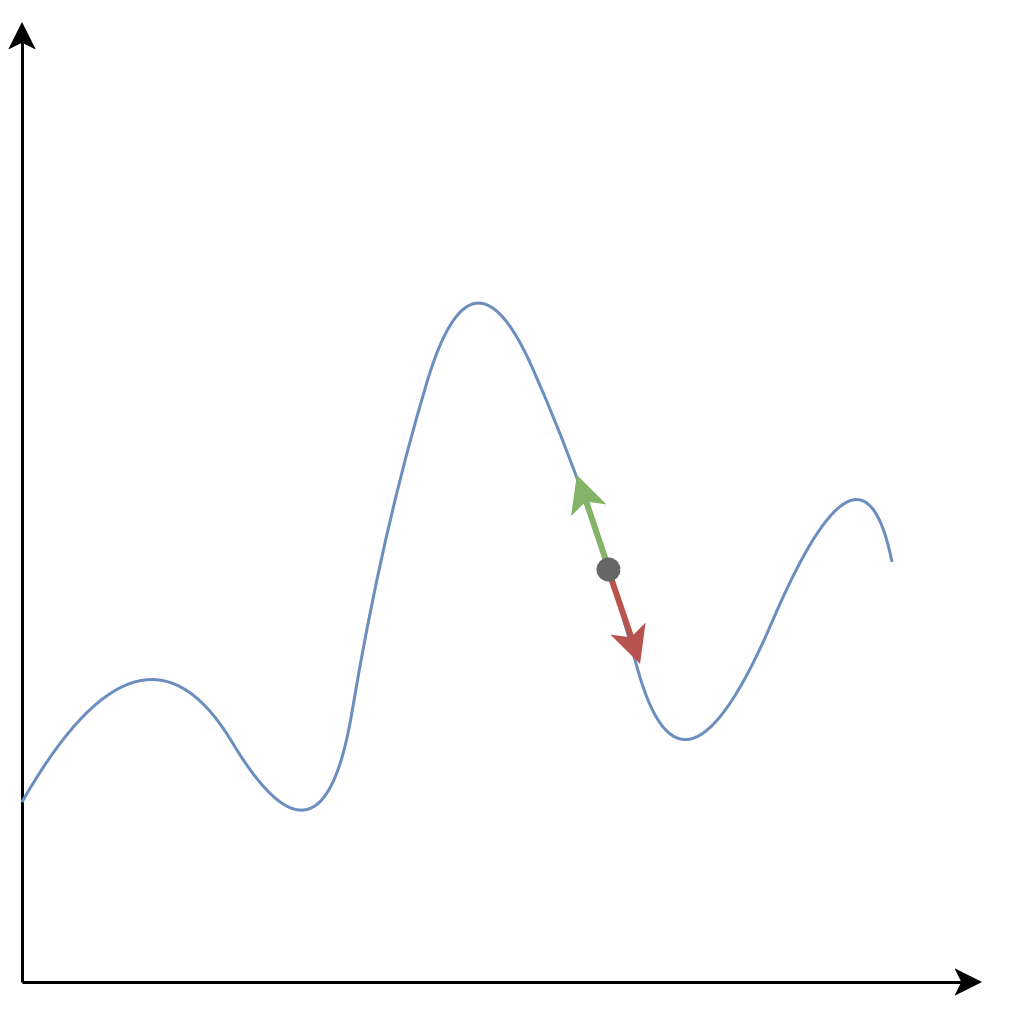
\includegraphics{2_1_points_gradients}
  \labfig{2_1}
  \caption[Gradient and Loss]{The gradient (green arrow) of a function evaluated
  in a specific point (gray) indicates the direction of the steepest ascent from
  that point. Conversely, the opposite of the gradient (red arrow) indicates the
  direction of the steepest descent. }
\end{marginfigure}

This method of using gradients to optimize function parameters, highlights a
crucial aspect of differentiable programming: every component of the
computational model, especially those that impact learning and prediction,
needs to be differentiable in terms of their parameters. Moreover, the
effectiveness of the optimization hinges directly on the efficiency with which
gradients are computed. Consequently, it is essential to have a robust method
for this computation to ensure the optimization process is both accurate and
efficient.

\subsection{Automatic Differentiation}
Automatic differentiation (AD) is a computational technique that efficiently
and accurately computes derivatives of functions. Unlike symbolic
differentiation, which manipulates mathematical symbols to produce derivative
formulas, or numerical differentiation, which approximates derivatives using
finite differences, AD operates directly on numerical values and applies the
chain rule to compute derivatives of composed functions. To fully understand
the utility and mechanics of Automatic Differentiation and the specific
challenges it addresses, it is crucial to first explore the two prevalent
methods used to compute derivatives on a computer. The first is \emph{symbolic
differentiation}, which involves manipulating the mathematical symbols of the
original expression through a set of transformation rules\sidenote{For
instance, the derivative $\frac{\partial \sin(x)}{\partial x}$ is $\cos(x)$.}.
By systematically applying these rules, one can derive an expression that can
be used to compute the gradient at any point, provided that the derivative is
continuous. Symbolic differentiation is considered stable in that it does not
introduce computational error. However, it is often challenging to implement
and can be computationally inefficient compared to other methods, particularly
as the function expressions become more complex and the expressions for their
derivatives increase drastically in the number of terms. This exponential
growth in complexity can significantly hinder performance and scalability.
The second approach to computing derivatives, known as \emph{numerical
differentiation} or the \emph{finite difference} method, utilizes the
conventional definition to calculate the derivative at
a specific point. \refeq{2_4} shows the standard formula for divided
differences, which calculates the slope of the secant line through the points
$(x,f(x))$ and $(x+h,f(x+h))$. By selecting an infinitesimally small value for
$h$, it is possible to achieve an increasingly accurate approximation of the
true derivative.
\begin{equation}
    \labeq{2_4}
    f'(x) = \lim_{h \to 0} \frac{f(x + h) - f(x)}{h}
\end{equation}
While generally being more computationally efficient than the former (as it
does not require the precomputation of the derivative expression), a
significant drawback of this approach is its numerical stability; it can
introduce round-off errors during the discretization process, particularly when
computing derivatives of orders higher than the first. This susceptibility to
errors stems from the finite precision with which computers represent numbers,
which can lead to inaccuracies in the calculated derivatives, especially for
small differences in function values.
\marginnote{Generally speaking, numerical differentiation is particularly
useful when the exact analytical derivative is difficult to obtain, as it
allows for the practical estimation of derivatives using straightforward
numerical computations.}

Both classical methods of differentiation, symbolic and numerical, have their
advantages and disadvantages. However, their primary drawback lies in the slow
computation of partial derivatives of a function with respect to multiple
inputs, which is essential for gradient-based optimization
algorithms\sidenote{Especially in deep learning, where the gradient with
respect to million of parameters must be computed at each iteration of the
learning process.}.
Automatic differentiation effectively resolves all these issues by providing a
more efficient and rapid means to calculate these derivatives, thereby
enhancing the performance of algorithms that rely heavily on gradient
calculations.

Automatic differentiation capitalizes on the principle that all functions,
regardless of their complexity, are ultimately reducible to a sequence of
elementary arithmetic operations (such as addition, subtraction, multiplication,
and division) and elementary functions (like exp, log, sin, and cos). The key
idea of AD involves breaking down computations into elementary steps that create
an \emph{evaluation trace} \sidecite{griewank_derivatives_2008}. Each step’s
derivative is then integrated using the chain rule. Thanks to the utilization of
evaluation traces, AD is capable of differentiating not only through
calculations in closed form but also through control flow statements commonly
found in programming. Regardless of the specific computational pathway executed,
the numerical operations will generate an evaluation trace that can be employed
for AD.
An evaluation trace can be seen as the series of steps that are needed to reach
the final result. Consider, for example, the function $f: \mathbb{R}^n \to
\mathbb{R}^m$ (where $n=2$ and $m=1$) whose expression is provided
in~\refeq{2_5}.
\begin{equation}
\labeq{2_5}
    y=\left[\sin \left(\frac{x_{1}}{x_{2}}\right)+\frac{x_{1}}{x_{2}}-\exp
    \left(x_{2}\right)\right] \left[\frac{x_{1}}{x_{2}}-\exp
    \left(x_{2}\right)\right]
\end{equation}
Using the following notation:
\begin{itemize}
    \item $v_{i-n} = x_i, i = 1, \dots, n$ are the input variables.
    \item $v_{i}, i=1, \dots, l$ are the intermediate variables.
    \item $y_{m-i} = v_{l-i}, i=(m-1), \dots, 0$ are the output variables.
\end{itemize}
\begin{margintable}[*-12] %[ht]
    \caption[Evaluation Trace]{Evaluation trace of \refeq{2_5}.}
    \labtab{2_1}
    \centering
    \resizebox{\textwidth}{!}{
    \begin{tabular}{ c c c }
      \toprule
      Variable & Expression & Value \\
      \midrule
        $v_{-1}$ & $x_1$ & $1.5$ \\
        $v_0$ & $x_2$ & $0.5$ \\
        $v_1$ & $v_{-1}/v_0$ & $3.0$ \\
        $v_2$ & $sin(v_1)$ & $0.141$ \\
        $v_3$ & $exp(v_0)$ & $1.648$ \\
        $v_4$ & $v_1 - v_2$ & $1.351$ \\
        $v_5$ & $v_2 + v_4$ & $1.492$ \\
        $v_6$ & $v_5 \cdot v_4$ & $2.016$ \\
      \bottomrule
    \end{tabular}
    }
\end{margintable}
The expression shown in \refeq{2_5} can be decomposed into simpler components as
shown in~\refeq{2_6}. By assigning values to each input, $x_1, x_2$, and
sequentially evaluating each sub-expression, the final value of $y$ can be
obtained\sidenote{This procedure corresponds to executing the differentiable
program $f$, a process often referred to in deep learning as the \emph{forward
pass}. This term underscores the transformation of the input signal through
intermediate steps until the output is reached}.
\begin{equation}
    \labeq{2_6}
    \begin{split}
        v_{-1} &= x_1\\
        v_0 &= x_2\\
        v_1 &= v_{-1} / v_0\\
        v_2 &= sin(v_1)\\
        v_3 &= exp(v_0)\\
        v_4 &= v_1 - v_3\\
        v_5 &= v_2 + v_4\\
        v_6 &= v_5 \cdot v_4\\
    \end{split}
\end{equation}
For example, a possible run with $x_1=1.5$ and $x_2=0.5$ would lead to the
evaluation trace depicted in \reftab{2_1}. This evaluation trace is also
called \emph{Wengert List} \sidecite{wengert_1964}.
A logical progression in determining the derivative of $y$ with respect to its
inputs involves following the evaluation trace and computing the derivatives
sequentially for each intermediate variable. This approach forms the basis of
the \emph{forward mode} of the automatic differentiation algorithm.
\begin{figure}
  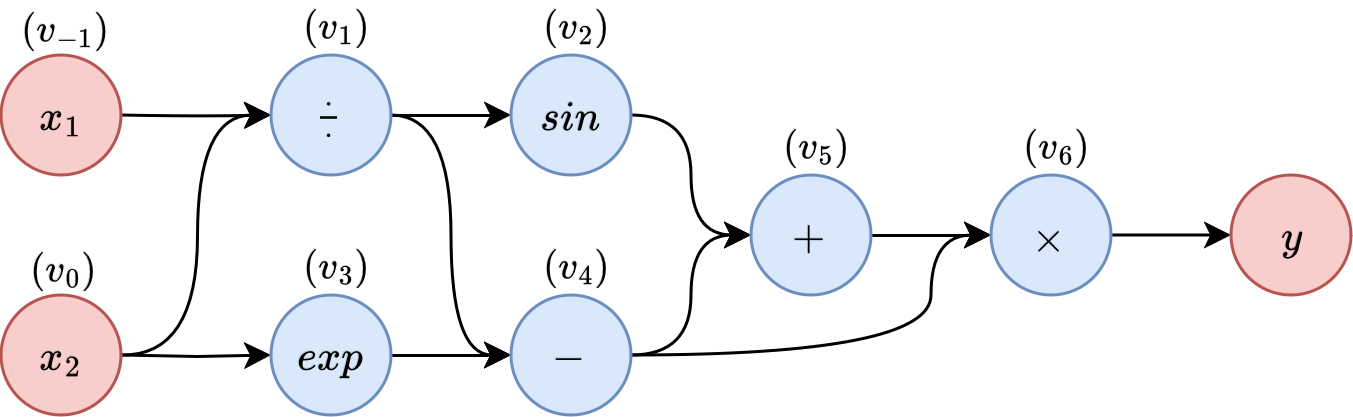
\includegraphics{2_2_computational_graph}
  \caption[Computational Graph]{\refeq{2_6} can also be represented
    graphically as a Directed Acyclic Graph (DAG). In this representation, blue
    nodes symbolize the intermediate operations, red nodes denote the
    input/output nodes, and the edges depict the algebraic relationships
    between these nodes.}
  \labfig{2_2}
\end{figure}
\subsubsection{Forward Mode}
Suppose the objective is to compute the derivative $\frac{\partial y}{\partial
t}$ with respect to an arbitrary input variable $t$. The chain rule
(\refeq{2_7}), offers a straightforward method for accomplishing this.
\begin{equation}
    \labeq{2_7}
    \der{u}{t} = \sum_i \left( \der{u}{v_i}\der{v_i}{t}\right)
\end{equation}\marginnote{\refeq{2_7} illustrates the application
of the chain rule in computing the gradient of $u$ with respect to any
intermediate variable $t$. The computation involves summing the products of
each partial derivative of $u$ with respect to its intermediate variables $v_i$
and the gradient of each intermediate variable $v_i$ with respect to the input
$t$.} The forward method of automatic differentiation involves calculating the
derivative $\dot{v}_i = \der{v_i}{t}$ for each intermediate variable
$v_i$. According to the chain rule (\refeqshort{2_7}), the derivative of each
variable $v_i$ is dependent on the values preceding it, allowing gradients to
be accumulated throughout the forward pass. This process is therefore aptly
named the \emph{forward accumulation mode}. To illustrate the dependency chain
integral to the process of forward accumulation,~\refeq{2_8}
demonstrates the computation of the derivative $\dot{v}_1$, emphasizing that
the current derivative value ($\dot{v}_1$) is contingent upon both the values
and derivatives of preceding variables ($v_0, v_{-1}$).
\begin{equation}
    \labeq{2_8}
    \begin{split}
        \dot{v}_1 &= \frac{\partial v_1}{\partial t}\\
        &= \frac{\partial v_1}{\partial v_{-1}}\frac{\partial v_{-1}}{\partial
        v_{t}} + \frac{\partial v_1}{\partial v_0}\frac{\partial
        v_0}{\partial v_t}\\
        &= \frac{\partial v_1}{\partial v_{-1}}\dot{v}_{-1} + \frac{\partial
        v_1}{\partial v_0}\dot{v}_0\\
        &= \frac{1}{v_0} \dot{v}_{-1} + \dot{v}_0 \left(-\frac{v_{-1}}{v_0^2}\right)
    \end{split}
\end{equation} By applying the same rule to each variable $v_i$, it is possible
to derive the formulas to compute the gradient of each intermediate variable of
the computation, as demonstrated in~\refeq{2_9}.
\begin{equation}
    \labeq{2_9}
    \begin{split}
        \dot{v}_{-1} &= \der{x_1}{t}\\
        \dot{v}_0 &= \der{x_2}{t}\\
        \dot{v}_1 &= \frac{1}{v_0}\dot{v}_{-1} + \dot{v}_0 \left(-\frac{v_{-1}}{v_0^2}\right)\\\
        \dot{v}_2 &= cos(v_1) \dot{v}_1\\
        \dot{v}_3 &= exp(v_0) \dot{v}_0\\
        \dot{v}_4 &= \dot{v}_1 - \dot{v}_3\\
        \dot{v}_5 &= \dot{v}_2 + \dot{v}_4\\
        \dot{v}_6 &= v_4\dot{v}_5 + v_5\dot{v}_4\\
    \end{split}
\end{equation}
\refeq{2_9} thus presents a generic method for computing the derivative
of $v_i$ with respect to any input variable $t$. \marginnote{In forward mode,
each node in the computational graph computes both the value of the node $v_i$
and its derivative $\dot{v}_i$.} To leverage this method, one must set the
derivative of the selected input variable relative to itself to $1$, while all
other input variable derivatives are set to $0$. Subsequently, both $v_i$ and
$\dot{v}_i$ are sequentially computed at each $i^{th}$ step. This approach
yields two outcomes for each computation: the value of the expression and its
derivative. The comprehensive record of derivative values is known as the
\emph{tangent trace}.

To illustrate this method, consider evaluating the derivative $\der{y}{x_1}$
($t=x_1$) at the point $x_1 = 1.5$ and $x_2 = 0.5$ using the forward
accumulation method. As discussed earlier, it is necessary to initialize
$\dot{v}_{-1} = 1$ (and accordingly $\dot{v}_0 = 0$) and proceed with a
sequential evaluation of the program\sidenote[][*-4]{Note that to obtain
$\der{y}{x_2}$, one must repeat the process, but setting $\dot{v}_0 = 1$ and
$\dot{v}_{-1} = 0$.}. The corresponding evaluation trace, along with its
tangent trace, is detailed in \reftab{2_2}.
\begin{margintable}
    \caption[Tangent Trace]{Evaluation trace of~\refeq{2_5} along with its
    tangent trace computed from~\refeq{2_9}.}
    \labtab{2_2}
    \centering
    \resizebox{\textwidth}{!}{
    \begin{tabular}{ c c c c }
      \toprule
      Variable & Value & Derivative \\
      \midrule
        $v_{-1}$ & $1.5$ & $1$ \\
        $v_0$ & $0.5$ & $0$\\
        $v_1$ & $3.0$ & $2$ \\
        $v_2$ & $0.141$ & $-1.98$\\
        $v_3$ & $1.648$ & $0$\\
        $v_4$ & $1.351$ & $0$\\
        $v_5$ & $1.492$ & $2$\\
        $v_6$ & $2.016$ & $3.01$\\
      \bottomrule
    \end{tabular}
    }
\end{margintable}
The forward accumulation method has been described using a function $f:
\mathbb{R}^2 \to \mathbb{R}^1$ but can be extended to any vector-valued real
function $f: \mathbb{R}^n \to \mathbb{R}^m$. This method is particularly
advantageous when $m \gg n$, because its computational complexity is $O(n)$,
correlating directly with the number of input dimensions of the function that
requires differentiation. This efficiency stems from the necessity to repeat
the forward and tangent computations for each input variable. Thus the forward
method is not suitable in the context of optimizations of neural networks,
where derivatives must be computed with respect to millions of parameters.
Specifically, in the context of deep neural networks optimization, the class
of vector valued functions are the loss functions, which have with a single
output $m=1$ and must be derived with respect to millions of parameters $n
\approx 10^6$.

\subsubsection{Reverse Mode}
Reverse mode automatic differentiation builds upon the concept that derivatives
can be computed from the end of the evaluation trace backwards to the beginning,
which is the reverse of the forward mode approach. This method is based on the
application of the chain rule (\refeq{2_7}), which, rather than being applied
from inputs to outputs, is utilized from outputs back to inputs. \refeq{2_10}
illustrates this principle, where $v_j$ represents all variables for which $v_i$
serves as an input, and $u$ denotes any output variable.
\begin{equation}
    \labeq{2_10}
    \der{u}{v_i} = \sum_j \left( \der{u}{v_j}\der{v_j}{v_i} \right)
\end{equation}
From a practical standpoint, reverse mode automatic differentiation (AD) does
not substantially differ from forward mode AD. It involves computing the
derivative $\bar{v}_i=\der{y}{v_i}$ for each intermediate variable, referred to
as the \emph{adjoint} of $v_i$. Utilizing~\refeq{2_10} simplifies this
process \sidenote{It is important to note that since the chain rule is applied
from the output back to the inputs, it must be executed in \emph{reverse
order}. This means that, unlike in forward mode where computation might start
with $v_0$ and $v_{-1}$, in reverse mode it begins from the final variable,
such as $v_6$.}.
\begin{equation}
    \labeq{2_11}
    \begin{split}
        \bar{v}_6 &= \der{y}{v_6} (=1)\\
        \bar{v}_5 &= \bar{v}_6 v_4\\
        \bar{v}_4 &= \bar{v}_6 v_5 + \bar{v}_5\\
        \bar{v}_3 &= -\bar{v}_4\\
        \bar{v}_2 &= \bar{v}_5\\
        \bar{v}_1 &= \bar{v}_4 + \bar{v}_2 cos(v_1)\\
        \bar{v}_0 &= \bar{v}_1 - \frac{v_{-1}}{v_0^2} + \bar{v}_3 \exp(v_0)\\
        \bar{v}_{-1} &= \frac{\bar{v}_2}{v_0}\\
    \end{split}
\end{equation}
\refeq{2_11} clearly demonstrates that in the computation of adjoints,
each step is dependent either on the values of subsequent steps or the adjoints
of these subsequent steps. Consequently, it is necessary to complete the
computations for $\bar{v}_i$ \emph{after} determining the values of $v_i$ and
the adjoints of subsequents steps $\bar{v}_k$ where $k > i$. Therefore, to
compute derivatives using this method, the entire expression must first be
executed to ascertain each $v_i$ value. Subsequently, the derivative of the
output variable with respect to itself must be initialized to 1, as exemplified
here with $\der{y}{v_6} = 1$. Following this initialization, the gradient
computations can proceed in reverse, beginning from the output variables and
progressing towards the input variables, following the same order
as~\refeq{2_11}.
\begin{figure*}
    \begin{subfigure}[h]{.5\linewidth}
        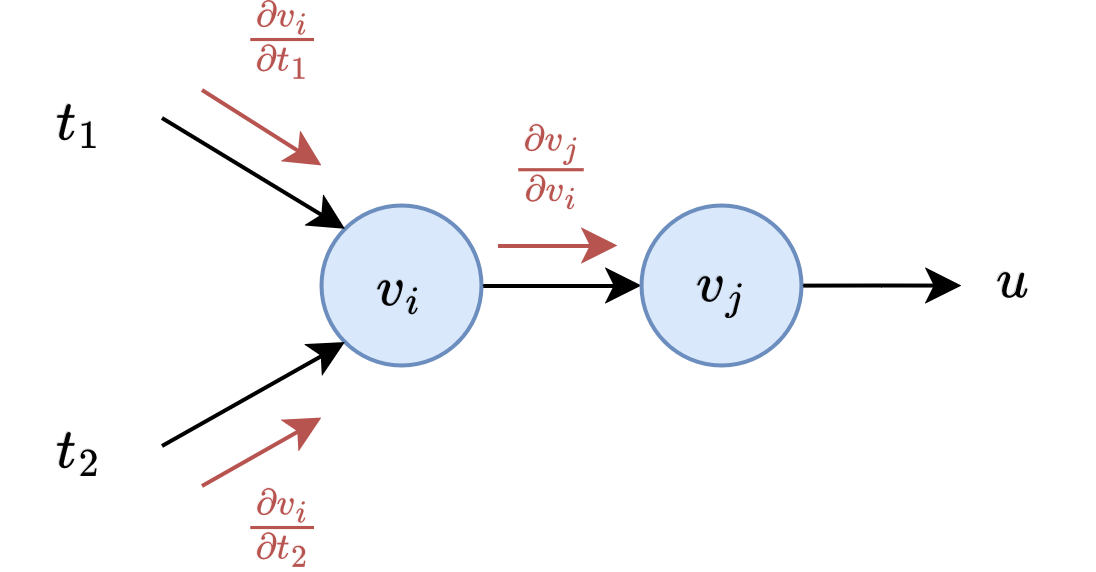
\includegraphics[width=1\linewidth]{2_3a_chain_rule_forward}
        \caption{Forward mode}
        \label{fig:3a}
    \end{subfigure}%
    \begin{subfigure}[h]{0.5\linewidth}
        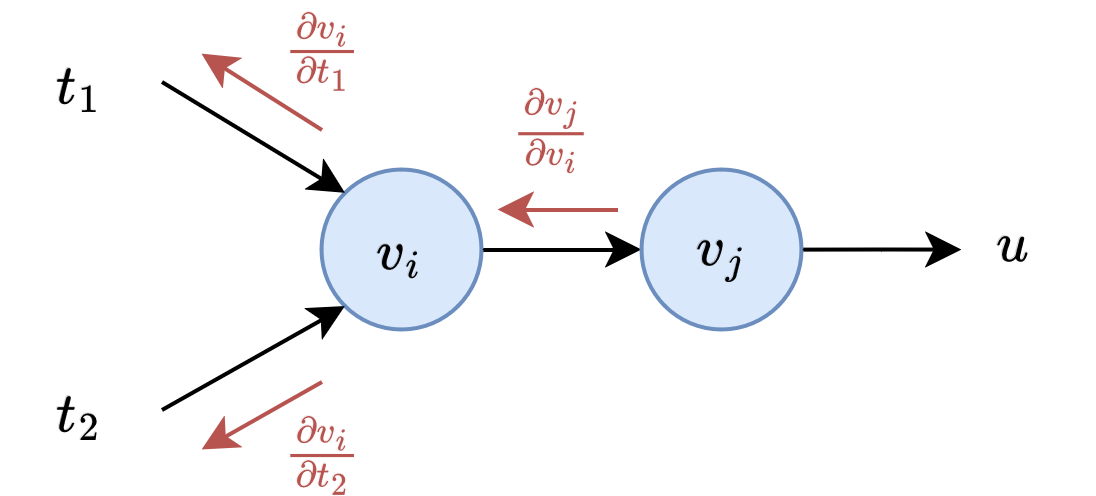
\includegraphics[width=1\linewidth]{2_3b_chain_rule_backward}
        \caption{Backward mode}
        \label{fig:3b}
    \end{subfigure}
    \caption[Chain Rule Forward-Backward Graph]{
        Graphically, interpreting the chain rule in forward mode involves
        propagating gradients from inputs to outputs. Subfigure~\ref{fig:3a}
        visually illustrates this process, showing how node $v_i$ transmits its
        derivative to the subsequent node $v_j$. Conversely, the backward mode
        entails the propagation of gradients from outputs back to inputs, as
        depicted in subfigure~\ref{fig:3b}. This graphical interpretation also
        clarifies how the automatic differentiation (AD) algorithm functions:
        to compute the derivative of a variable $u$ with respect to another
        variable $t$, it simply involves multiplying the gradients that appear
        along the path from $u$ to $t$.
    }
\end{figure*}

Upon completing the backward mode of automatic differentiation, the adjoints of
the input variables are determined. These adjoints represent the partial
derivatives of $y$ with respect to the input variables. This aspect underscores
the efficiency of the reverse method: a single application of reverse mode
yields the gradients for all input variables. With only two traversals of the
computation graph (one forward and one backward) the method achieves a
computational complexity of $O(2n)$. This efficiency makes it particularly
suitable for computing the gradients of loss functions with respect to the
parameters in deep neural networks\sidenote{In the context of deep learning,
reverse mode automatic differentiation is commonly referred to as
\emph{backpropagation}.}, a crucial step in gradient-based optimization. Today,
reverse mode automatic differentiation is the de facto standard for computing
derivatives in the field. Common deep learning frameworks (or AD engines) such
as PyTorch \sidecite{paszke_2017} and TensorFlow \sidecite{abadi_2016}
internally represent computations as graphs and apply reverse mode automatic
differentiation to compute the derivatives on these graphs.

Reverse mode automatic differentiation (AD) is highly efficient for computing
gradients, but it does have a drawback concerning memory efficiency. Since the
values of each intermediate step need to be available before initiating the
backward pass, the entire evaluation trace must be stored in memory. This
requirement can become unfeasible, particularly when dealing with large
datasets or deep neural network models that involve extensive computational
graphs. Such memory demands can limit the scalability of reverse mode AD in
resource-constrained environments or when training extremely large models.
\subsection{Stochastic Gradient Descent}
As previously mentioned, gradient-based optimization methods compute the
gradient of the expected loss with respect to the model's parameters. By
examining the update rule in~\refeq{2_3}, it is evident that the
gradient computation of the expected loss can become problematic. This is due
to the fact that, as the dataset size increases, memory and computational
requirements for reverse mode automatic differentiation to compute the gradient
would escalate significantly, rendering the method impractical for extremely
large datasets. In practical applications, a variant of gradient descent known
as Stochastic Gradient Descent (SGD) is commonly used. The fundamental concept
of SGD involves sampling a subset $\mathcal{B}_r \subset \mathcal{D}_n$ (where
$r \ll n$) at each iteration $t$. Utilizing this subset allows for the
computation of an approximated version of the true expected loss, as
demonstrated in~\refeq{2_12}.
\begin{equation}
    \labeq{2_12}
    \frac{1}{r} \sum_{(x_i, y_i) \in \mathcal{B}_r} L(y_i, f(x_i; \theta)) \approx 
    \frac{1}{n} \sum_{(x_i, y_i) \in \mathcal{D}_n} L(y_i, f(x_i; \theta)) 
\end{equation}
If the samples of the minibatch are independent and identically distributed
from the dataset, the left-hand side of~\refeq{2_12} constitutes a
Monte Carlo approximation of the full loss, and the same principle also applies
to its gradient. The computational complexity of this process grows only with
$r$, which users can directly control\sidenote[][*-12]{In practical terms,
selecting smaller minibatch sizes ($r$) leads to more computationally efficient
iterations but introduces higher variance in the gradient estimates. Conversely,
larger $r$ values produce more accurate gradient estimations but result in less
efficient iterations. This trade-off between efficiency and accuracy must be
carefully managed to optimize the learning process.}.

\section{Neural Networks}
Now that the foundational knowledge on how to train deep learning models has
been established, the focus shifts to the models themselves. Previously, the
model was defined as a plain function to abstract away the real components and
inner workings, which will be discussed extensively in this section. Neural
networks vary from simple to highly complex architectures, each possessing
distinct capabilities and applications. However, all of these architectures are
constructed with high-level differentiable components, such as neurons and
layers\sidenote{To draw a parallel with conventional programming, these
components can be seen as the basic constructs of differentiable programming.}.

\subsection{Perceptron}
The Perceptron \sidecite{rosenblatt_1958} represents one of the earliest models
in the field of artificial neural networks, and serves as the basic building
block the complex models that can be found today. The perceptron draws
inspiration by the biological neuron, which, in a simplified view, functions by
receiving a series of electrical input signals (coming from other neurons) that
are collectively processed\sidenote{Synaptic strengths, or synaptic weights,
determine the influence of one neuron's signal on another.}. These synaptic
weights can change through a process called synaptic plasticity, which is
crucial for learning and memory.
The perceptron mimics this mechanism with these main components:
\begin{itemize}
    \item \textbf{Input nodes}: a vector $\mathbf{x}$ whose the single entry
    $x_i$ represents the signal strength coming from the $i^{th}$ input.
    \item \textbf{Weights}: a vector $\mathbf{w}$ that determines the synaptic
    strength of each input.
    \item \textbf{Bias}: a real value $b$ that can be likened to the neuron's
    resting membrane potential\sidenote{The resting membrane potential is the
    baseline level of electrical charge inside the neuron relative to the
    outside.}.
    \item \textbf{Activation function}: a real valued function $\sigma:
    \mathbb{R} \to \mathbb{R}$ that determines whether the perceptron will
    activate or not based on its activation field\sidenote{The activation field
    of a perceptron is the weighted sum of the inputs plus the bias}.
\end{itemize}
\refeq{2_13} shows the output of the perceptron model, utilizing all the
previously discussed components. Note that the function is parameterized by the
vector of weights and the bias. Consequently, the optimization process will
adjust these parameters to enable the model to learn effectively.
\begin{equation}
    \labeq{2_13}
    \begin{split}
    f(\mathbf{x}; \mathbf{w}, b) &= \sigma \left( b + \sum_{i} \mathbf{w}_i \cdot \mathbf{x}_i \right)\\
    &= \sigma (b + \mathbf{w} \cdot \mathbf{x})
    \end{split}
\end{equation}
Frequently, another formulation for the perceptron model is preferred, where the
bias term $b$ is \emph{"absorbed"} into the weight vector $\mathbf{w}$ by
setting the first weight variable $\mathbf{w}_0 = b$ and fixing the first input
entry to always be $x_0 = 1$. The resulting formulation in~\refeq{2_14}
is equivalent to that in~\refeq{2_13}, offering a more compact notation that
simplifies readability.
\begin{equation}
    \labeq{2_14}
    \begin{split}
    f(\mathbf{x}; \mathbf{w}) &= \sigma \left( \sum_{i} \mathbf{w}_i \cdot \mathbf{x}_i \right)\\
    \end{split}
\end{equation}
The perceptron model is particularly adept at solving linear classification
problems by identifying a hyperplane that separates data points into two
distinct classes within a multidimensional space. It excels in scenarios where
the classes can be divided by a straight line in two dimensions, a plane in
three dimensions, or a hyperplane in higher dimensions. If such a hyperplane
exists, the perceptron model will eventually converge to a solution that
accurately classifies all the training examples.
\begin{marginfigure}[*-8]
  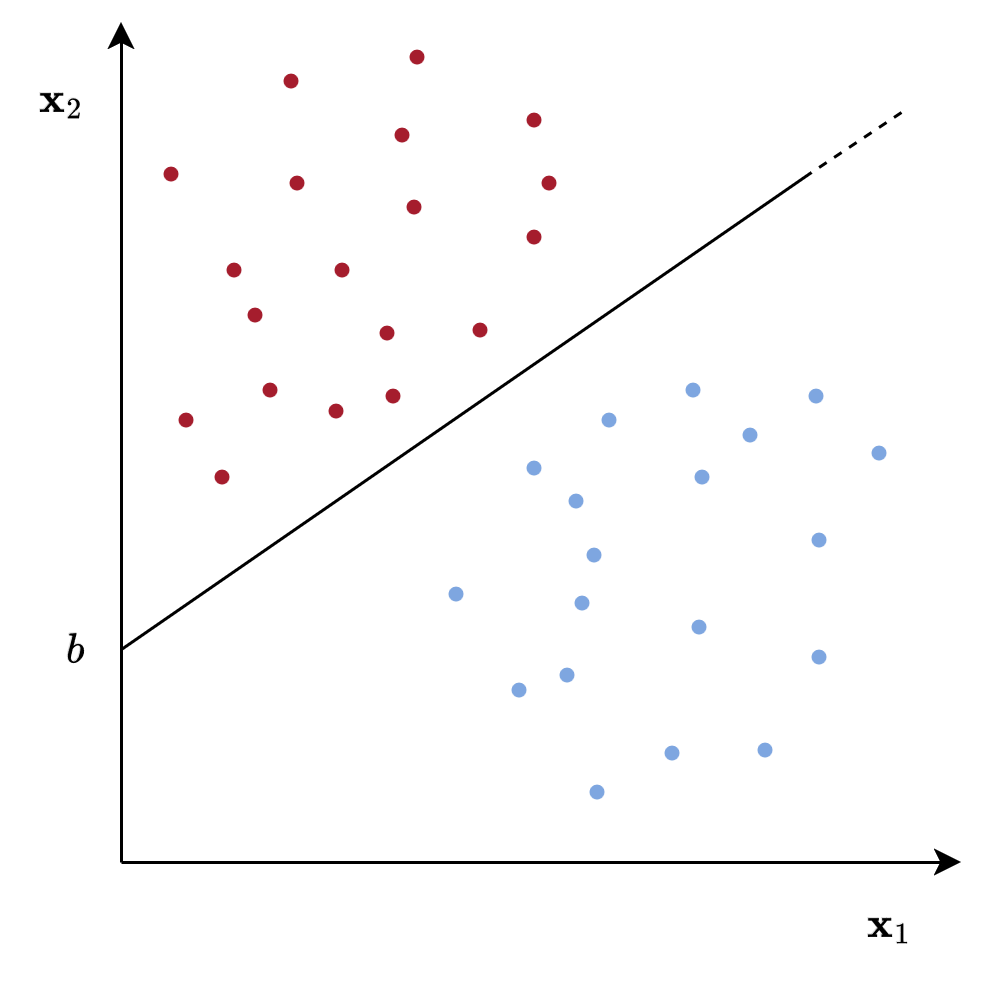
\includegraphics{2_4_linearly_separable}
  \labfig{2_4}
  \caption[Linearly Separable Problem]{
  An example of a linearly separable problem. In this case, $\mathbf{x}$ has
  only 2 elements. The perceptron model creates a line (decision boundary) that
  perfectly separates the examples.
  }
\end{marginfigure}
Common examples of linearly separable problems include binary classification
tasks, such as distinguishing between spam and non-spam emails or identifying
positive versus negative sentiment in text. Additionally, the perceptron can
effectively learn certain Boolean functions, like AND and OR, where the output
can be separated linearly based on the inputs.
\begin{figure}[h]
  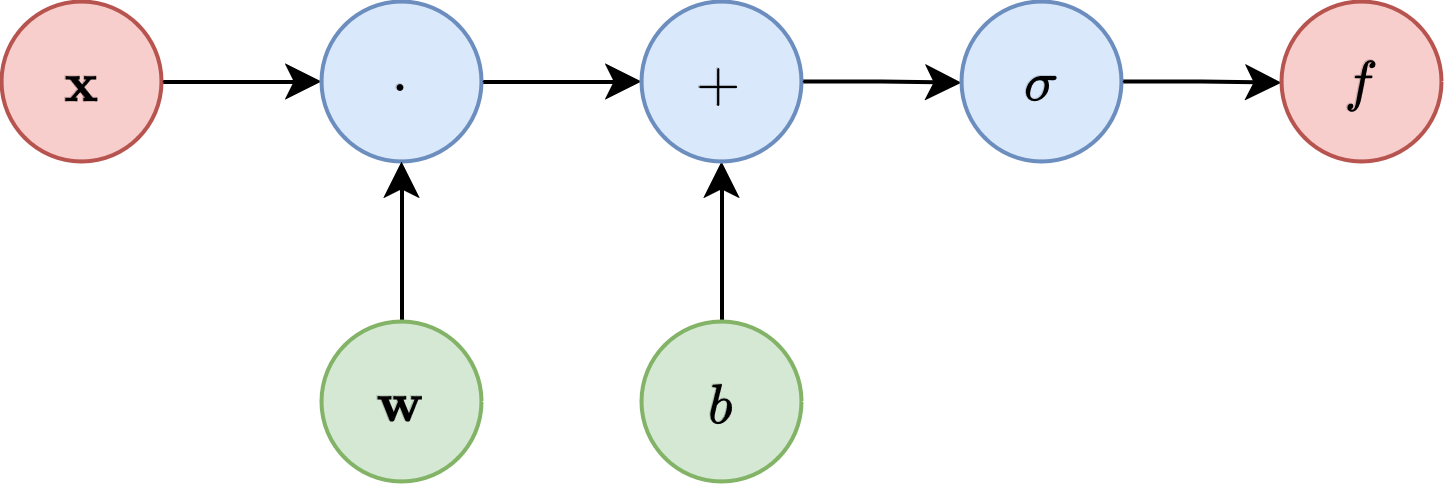
\includegraphics{2_5_perceptron_computational_graph}
  \labfig{2_5}
  \caption[Perceptron Computational Graph]{
      Computational graph of a perceptron. Blue nodes represents
      operators/function, red nodes input/output nodes and green nodes function
      parameters
  }
\end{figure}
Despite its strengths, the perceptron model has notable limitations,
particularly when it comes to handling non-linearly separable problems. In cases
where no single hyperplane can effectively separate the classes, the perceptron
algorithm fails to converge to an accurate solution. A classic example of this
limitation is the XOR problem, where the classes are not linearly separable, and
thus, the perceptron is unable to find a suitable decision boundary. A graphic
example of a non linearly separable problem is depicted in~\reffig{2_6}.
\begin{marginfigure}[*-6]
  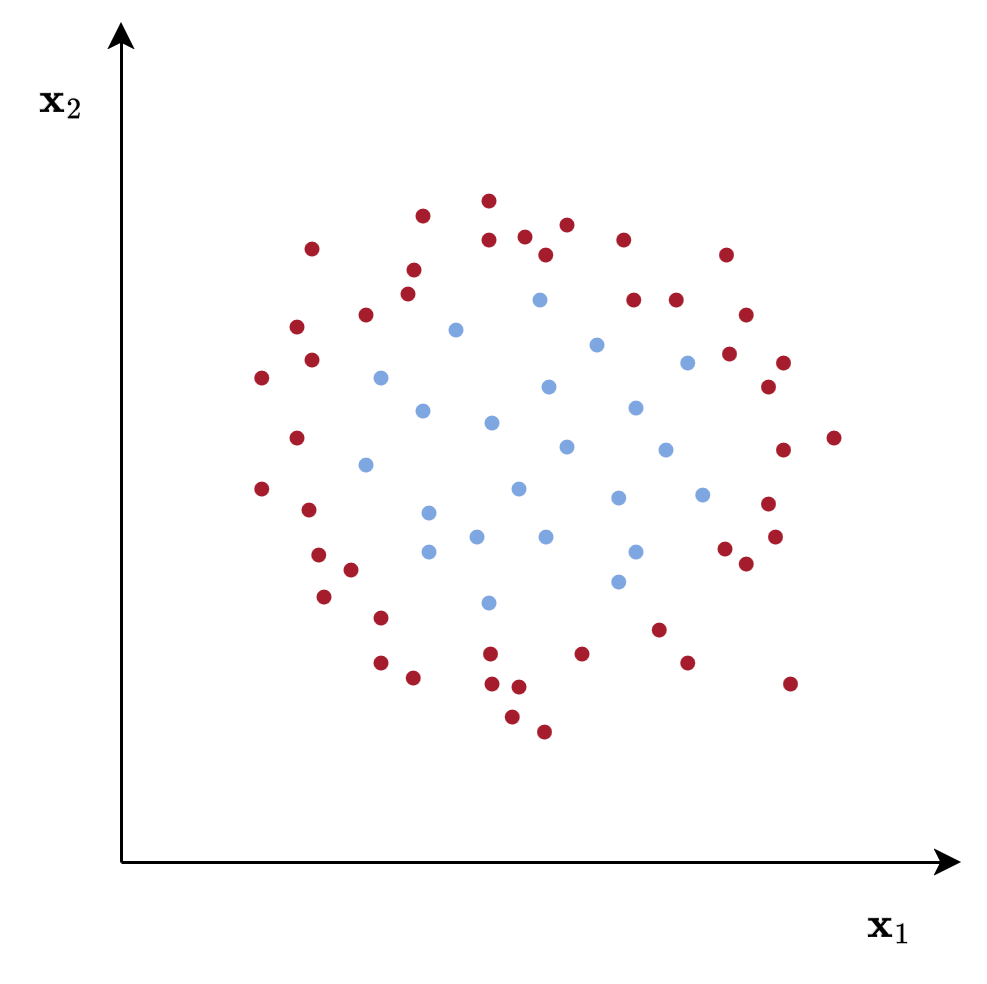
\includegraphics{2_6_non_linearly_separable}
  \caption[Non Linearly Separable Problem]{
  An example of a non linearly separable problem. No line can separate clearly
  the red class from the blue class.
  }
  \labfig{2_6}
\end{marginfigure}
The inability to solve non-linear problems restricts the applicability of the
perceptron model to only a subset of classification tasks, a limitation that
arises from the linear nature of the decision boundary that the perceptron
attempts to establish\sidenote[][*4]{The activation field of a perceptron is in
fact the expression of a line/plane/hyperplane.}.
Many practical problems exhibit non-linear separability, rendering the perceptron
model unsuitable for numerous real-world tasks. Despite the inherent limitations
of the perceptron, it serves as a fundamental building block of neural networks.
By integrating multiple perceptrons, it is possible to construct a fully
connected layer, thereby enhancing the model's capacity to address more complex
tasks.

\subsection{Multi-Layer Perceptron}
Using the perceptron as a foundational element, it is possible to construct a
more sophisticated and general entity: a fully connected layer. A fully
connected layer, also referred to as a network layer, consists of $n$ stacked
perceptrons that share the same inputs. As outlined in~\refeq{2_15}, the
parameters of this layer are encapsulated within a matrix $\mathbf{W} \in
\mathbb{R}^{(n \times m)}$, where $n$ represents the number of perceptrons and
$m$ denotes the number of inputs. Each row of the matrix $\mathbf{W}$ corresponds
to the weight vector $\mathbf{w}$ of an individual perceptron. Furthermore, the
output from this layer is a vector of $n$ elements, with each element reflecting
the output from the corresponding perceptron.
\begin{equation}
  \labeq{2_15}
  F(\mathbf{x}; \mathbf{W}) = (f(\mathbf{x}; \mathbf{W}_1), \dots, f(\mathbf{x}; \mathbf{W}_n))
\end{equation}
Instead of computing the output of each perceptron indipendently, it is possible
to compute the output of all perceptrons of the entire layer in parallel, with
just one matrix-vector multiplication as shown in~\refeq{2_16}.
\begin{equation}
    \labeq{2_16}
    F(\mathbf{x}; \mathbf{W}) = \sigma \left( \mathbf{W} \cdot \mathbf{x} \right )
\end{equation}
By utilizing this new construct, it is possible to develop arbitrarily powerful
models. Each layer, being a function, can be composed with other layers to
facilitate sequential computations. In this manner, the output of one layer
becomes the input for the next layer, akin to function composition. 
\begin{equation}
    \labeq{2_17}
    \mathcal{N}(\mathbf{x}; \theta) = (F_1 \circ \dots \circ F_d)(\mathbf{x})
\end{equation}
\marginnote{All layers between $F_i$ with $i \in 2 \dots d$ are called
\emph{hidden layers}.}
\refeq{2_17} formalizes this concept. The resulting model is a fully connected
multi-layered neural network with $d$ layers. Each fully connected layer $F_i$
is parametrized by a weight matrix $\mathbf{W}_i \in \theta$, where $\theta$
represents the set of all parameters of the model.

The models constructed with this framework are called Multilayer Perceptrons
(MLP) \sidecite{rosenblatt_1959} or Feedfoward Neural Networks (FNN). The main
idea of stacking one layer after another in a feedforward network is to enable
the model to learn a hierarchical mapping of the data. For example, in the XOR
problem, a single-layer perceptron fails because it cannot find a linear
boundary to separate the classes. However, by introducing additional layers,
each layer can learn to transform the input data into a more suitable
representation. The first layer might learn simple features, which are then
combined and transformed by subsequent layers into more complex features. This
hierarchical learning allows the network to create intermediate representations
that progressively disentangle the input data, ultimately enabling the final
layer to classify the data accurately. Thus, the network effectively maps the
original input space into a new space where the classes become linearly
separable.

By mapping inputs into diffeerent high-dimensional spaces, FNNs are able to
learn effectively any non-linear problem. In fact, it has been proven that any
feedforward network composed of two layers can approximate any continuous
function on compact subsets of $\mathbb{R}^n$ to arbitrary accuracy, provided it
has a sufficient number of neurons and the appropriate activation functions
\sidecite{leshno_1993}. Feedforward networks are therefore said to be
\emph{universal approximators}.

\subsection{Convolutional Networks}
While the extreme generality of feedforward models (due to their ability to
approximate any function), makes these models very powerful, it also introduces
an additional problem. To illustrate this, consider that each model
configuration $\theta$ of a feedforward network (FFN) represents a point in the
high-dimensional space of all possible model configurations called the
\emph{hypotheses space}. In this vast configuration space, only a small subspace
is relevant for solving the specific problem at hand (i.e., configurations that
make the model perform the chosen task). However, as the number of parameters in
the network grows, the dimensionality of this space increases, leading to an
exponential explosion of possible configurations for the optimization method to
explore. \marginnote{Another problem also arises from the high time and space
complexity of gradient computations, which grows linearly with the number of
parameters, but the parameters themselves of a feedforward network grow
exponentially as the number of neurons increases.}

To mitigate this issue, FFNs are deliberately made less powerful by encoding
inductive priors into the model. Inductive priors are assumptions about the type
of data the model will process and the tasks it must solve. By incorporating
these priors, the expressive power of the models is effectively constrained,
\emph{limiting} the space of all possible configurations. This confinement helps
gradient-based optimization methods focus on regions containing plausible
solutions to the problem at hand.

Convolutional Neural Networks (CNNs)
\sidecite{lecun_cnn_1989}\cite{fukushima_neocognitron_1980} are a type of neural
network architecture that encode specific inductive priors, facilitating the
processing of image data. These priors are:
\begin{itemize}
    \item \textbf{Locality}: image data consists of pixel values where nearby
    pixels are more related than distant ones\sidenote{For example, in an image
    representing a line, pixels will have similar values along the direction of
    the line.}.
    \item \textbf{Weight Sharing}: neurons in the same layer share weights,
    reducing the total number of parameters required for a layer.
    \item \textbf{Pooling}: high-level features (e.g., objects, lines) in an
    image are meaningful only when interpreted over a sufficiently large patch
    of pixels.
\end{itemize}
To encode the first two priors, CNNs utilize a specific type of
layer\sidenote{Recall that layers in neural networks can be seen as the
constructs of a differentiable programming language.} called the
\emph{Convolutional Layer}, which is the origin of their name.

\subsubsection{Convolutional Layer}
Such layer implements a \emph{convolution}, a mathematical operation that (in
the discrete case) consists on computing the sum of the product between two
functions after one is reflected about the $y$-axis and shifted.
\begin{marginfigure}[*-4]
    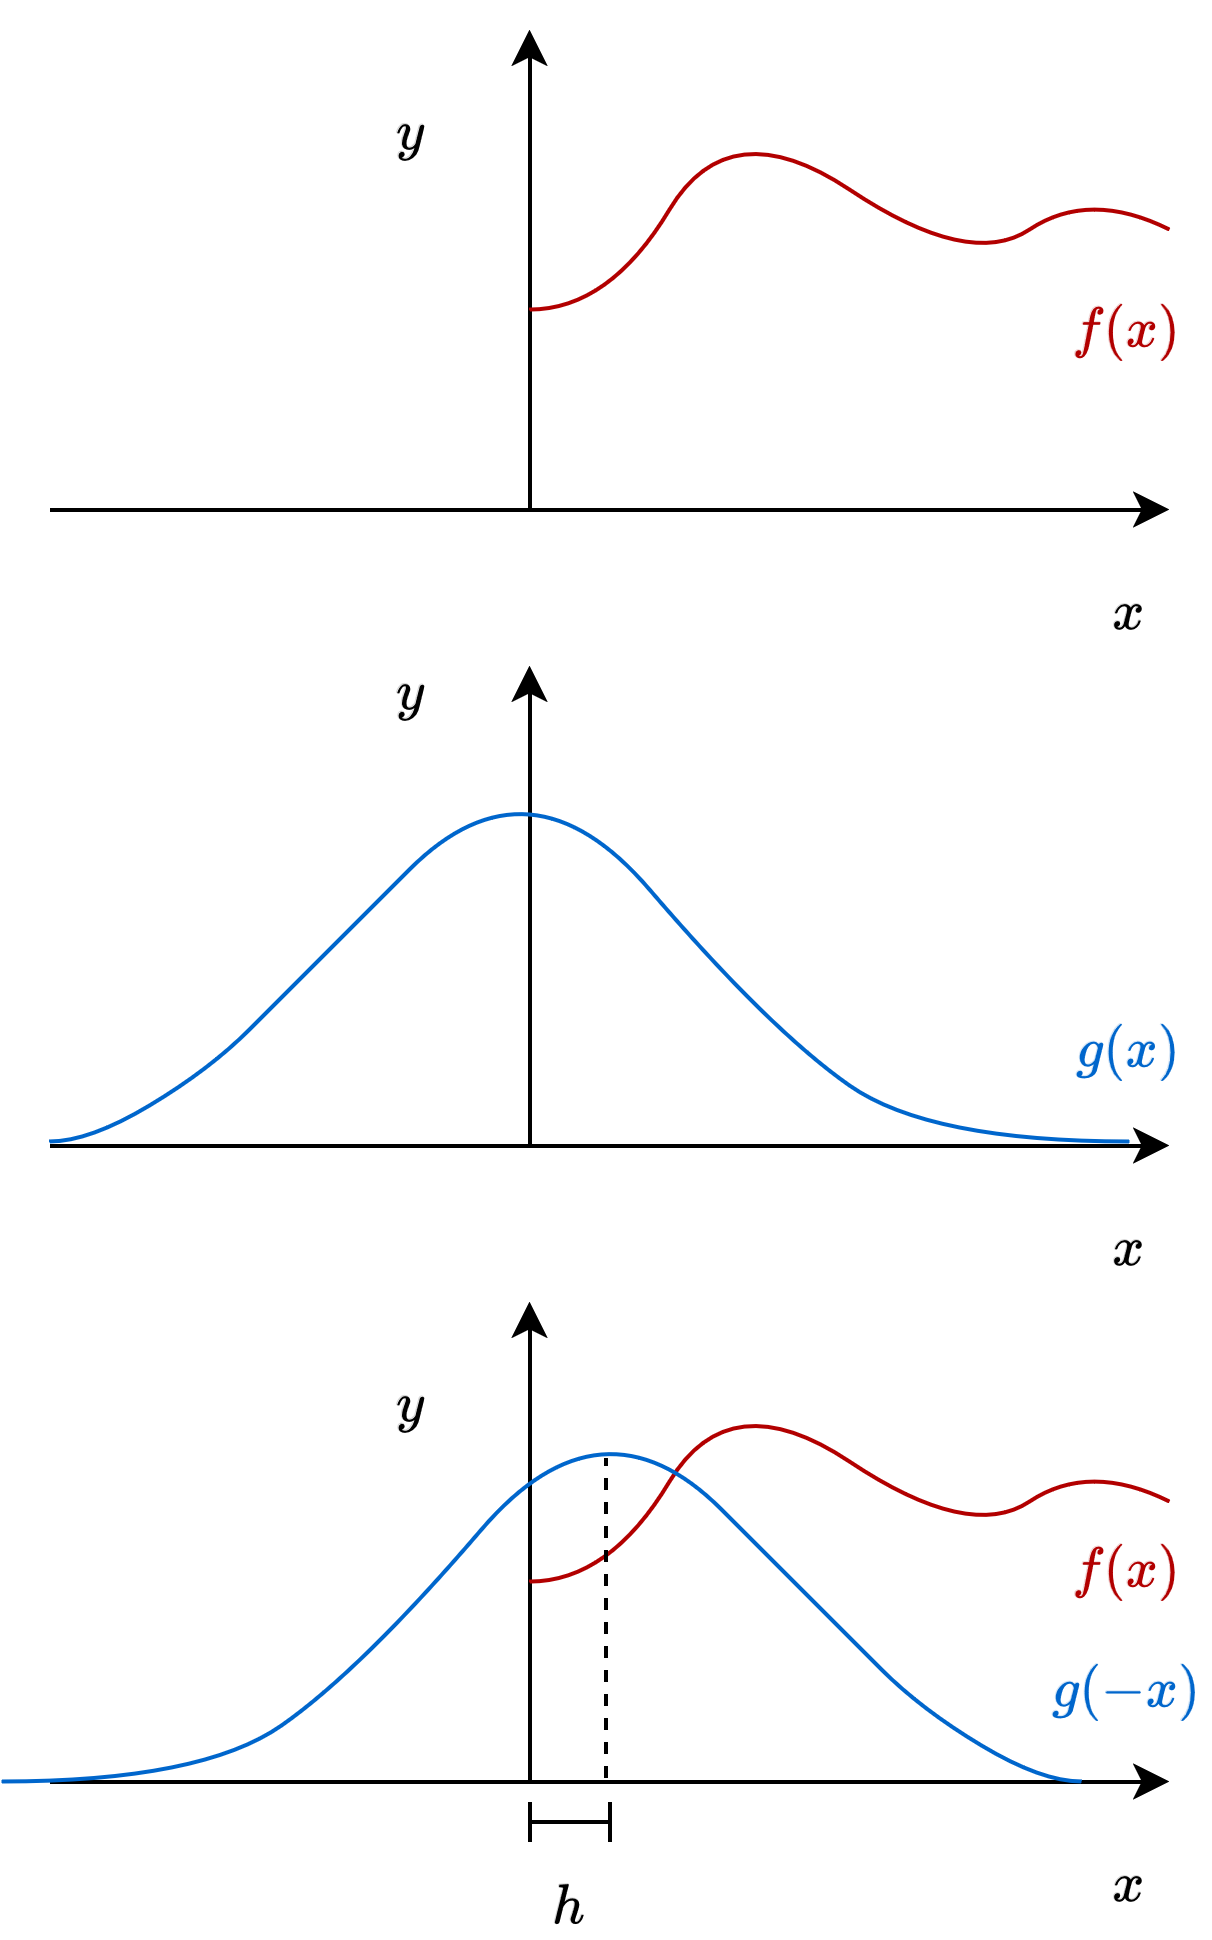
\includegraphics{2_7_convolution_1d}
    \labfig{2_7}
    \caption[Convolution (Mathematical Operation) in 1D]{
    Example of the convolution operation in one dimension. Note that in the
    convolution, $g$ is flipped horizontally ($g(-x)$) and slid over $f$ by a
    displacement $h$.
    }
\end{marginfigure}
From~\refeq{2_18} it can be seen that the convolution actually consists on
computing the similarity between two functions, making one of the function to
progressively slide over the $x$ dimension.
\begin{equation}
    \labeq{2_18}
    (f \star g)(x) = \sum^\infty_{h=-\infty} f(x)g(x - h) 
\end{equation}
The convolution layer implements this operation, where $f$ is the input image
and $g$ (also called the \emph{kernel}) are the learnable parameters (weights)
of the layer. Since images are 2-dimensional bounded discrete
functions\sidenote[][*8]{Images can be seen as the the sampled version of a
2-dimensional real valued signal}, the operation is applied over both
dimensions. \refeq{2_19} shows the output of a single convolutional
neuron. 
\begin{equation}
    \labeq{2_19}
    C(\mathbf{X}; \mathbf{W})_{x, y} = \sum^{M/2}_{m=-M/2}\sum^{N/2}_{n=-N/2}
    \mathbf{X}_{x, y}\mathbf{W}_{(x - m), (y - n)} 
\end{equation}

In~\refeq{2_19}, $M \times N$ represents the dimensions of the
kernel\sidenote[][*4]{Which are typically much smaller than the input image
size.} $\mathbf{W}$ and $\mathbf{X}_{x, y}$ the value of the $(x, y)$ pixel of
the input image. Note that since the input is 2-dimensional, even the neurons
are arranged in a grid-like manner. That is why each neuron's output is
indicized by the variables $x$ and $y$. The results of the convolutional layer
is then also a matrix, called \emph{feature map}. From~\refeq{2_19} it is also
clear how the locality prior is effectively encoded: each neuron process only a
subset of the input\sidenote{That corresponds to a window with dimension $M
\times N$, centered at the $(x, y)$ position.}. The second prior is explained by
the fact that each value of $\mathbf{W}$ is shared between each neuron. That is,
for a single convolutional layer, there exists only an $M \times
N$\sidenote{Without counting other factors such as the sliding window and the
number of channels.} matrix of parameters, which, as previously mentioned, is
much smaller than the input size. The number of parameters of a convolutional
layer is therefore much smaller than its fully connected counterpart.

To be precise, image data is composed of multiple channels which are commonly 3:
red, green and blue. The extension for the convolution layer is straightforward,
it is sufficient to apply the convolution on an additional dimension which
represent the channel, thus, for RGB images, convolutional filters are typically
matrices with dimensions $M \times N \times 3$, where $3$ is the number of
channels.
\begin{marginfigure}
  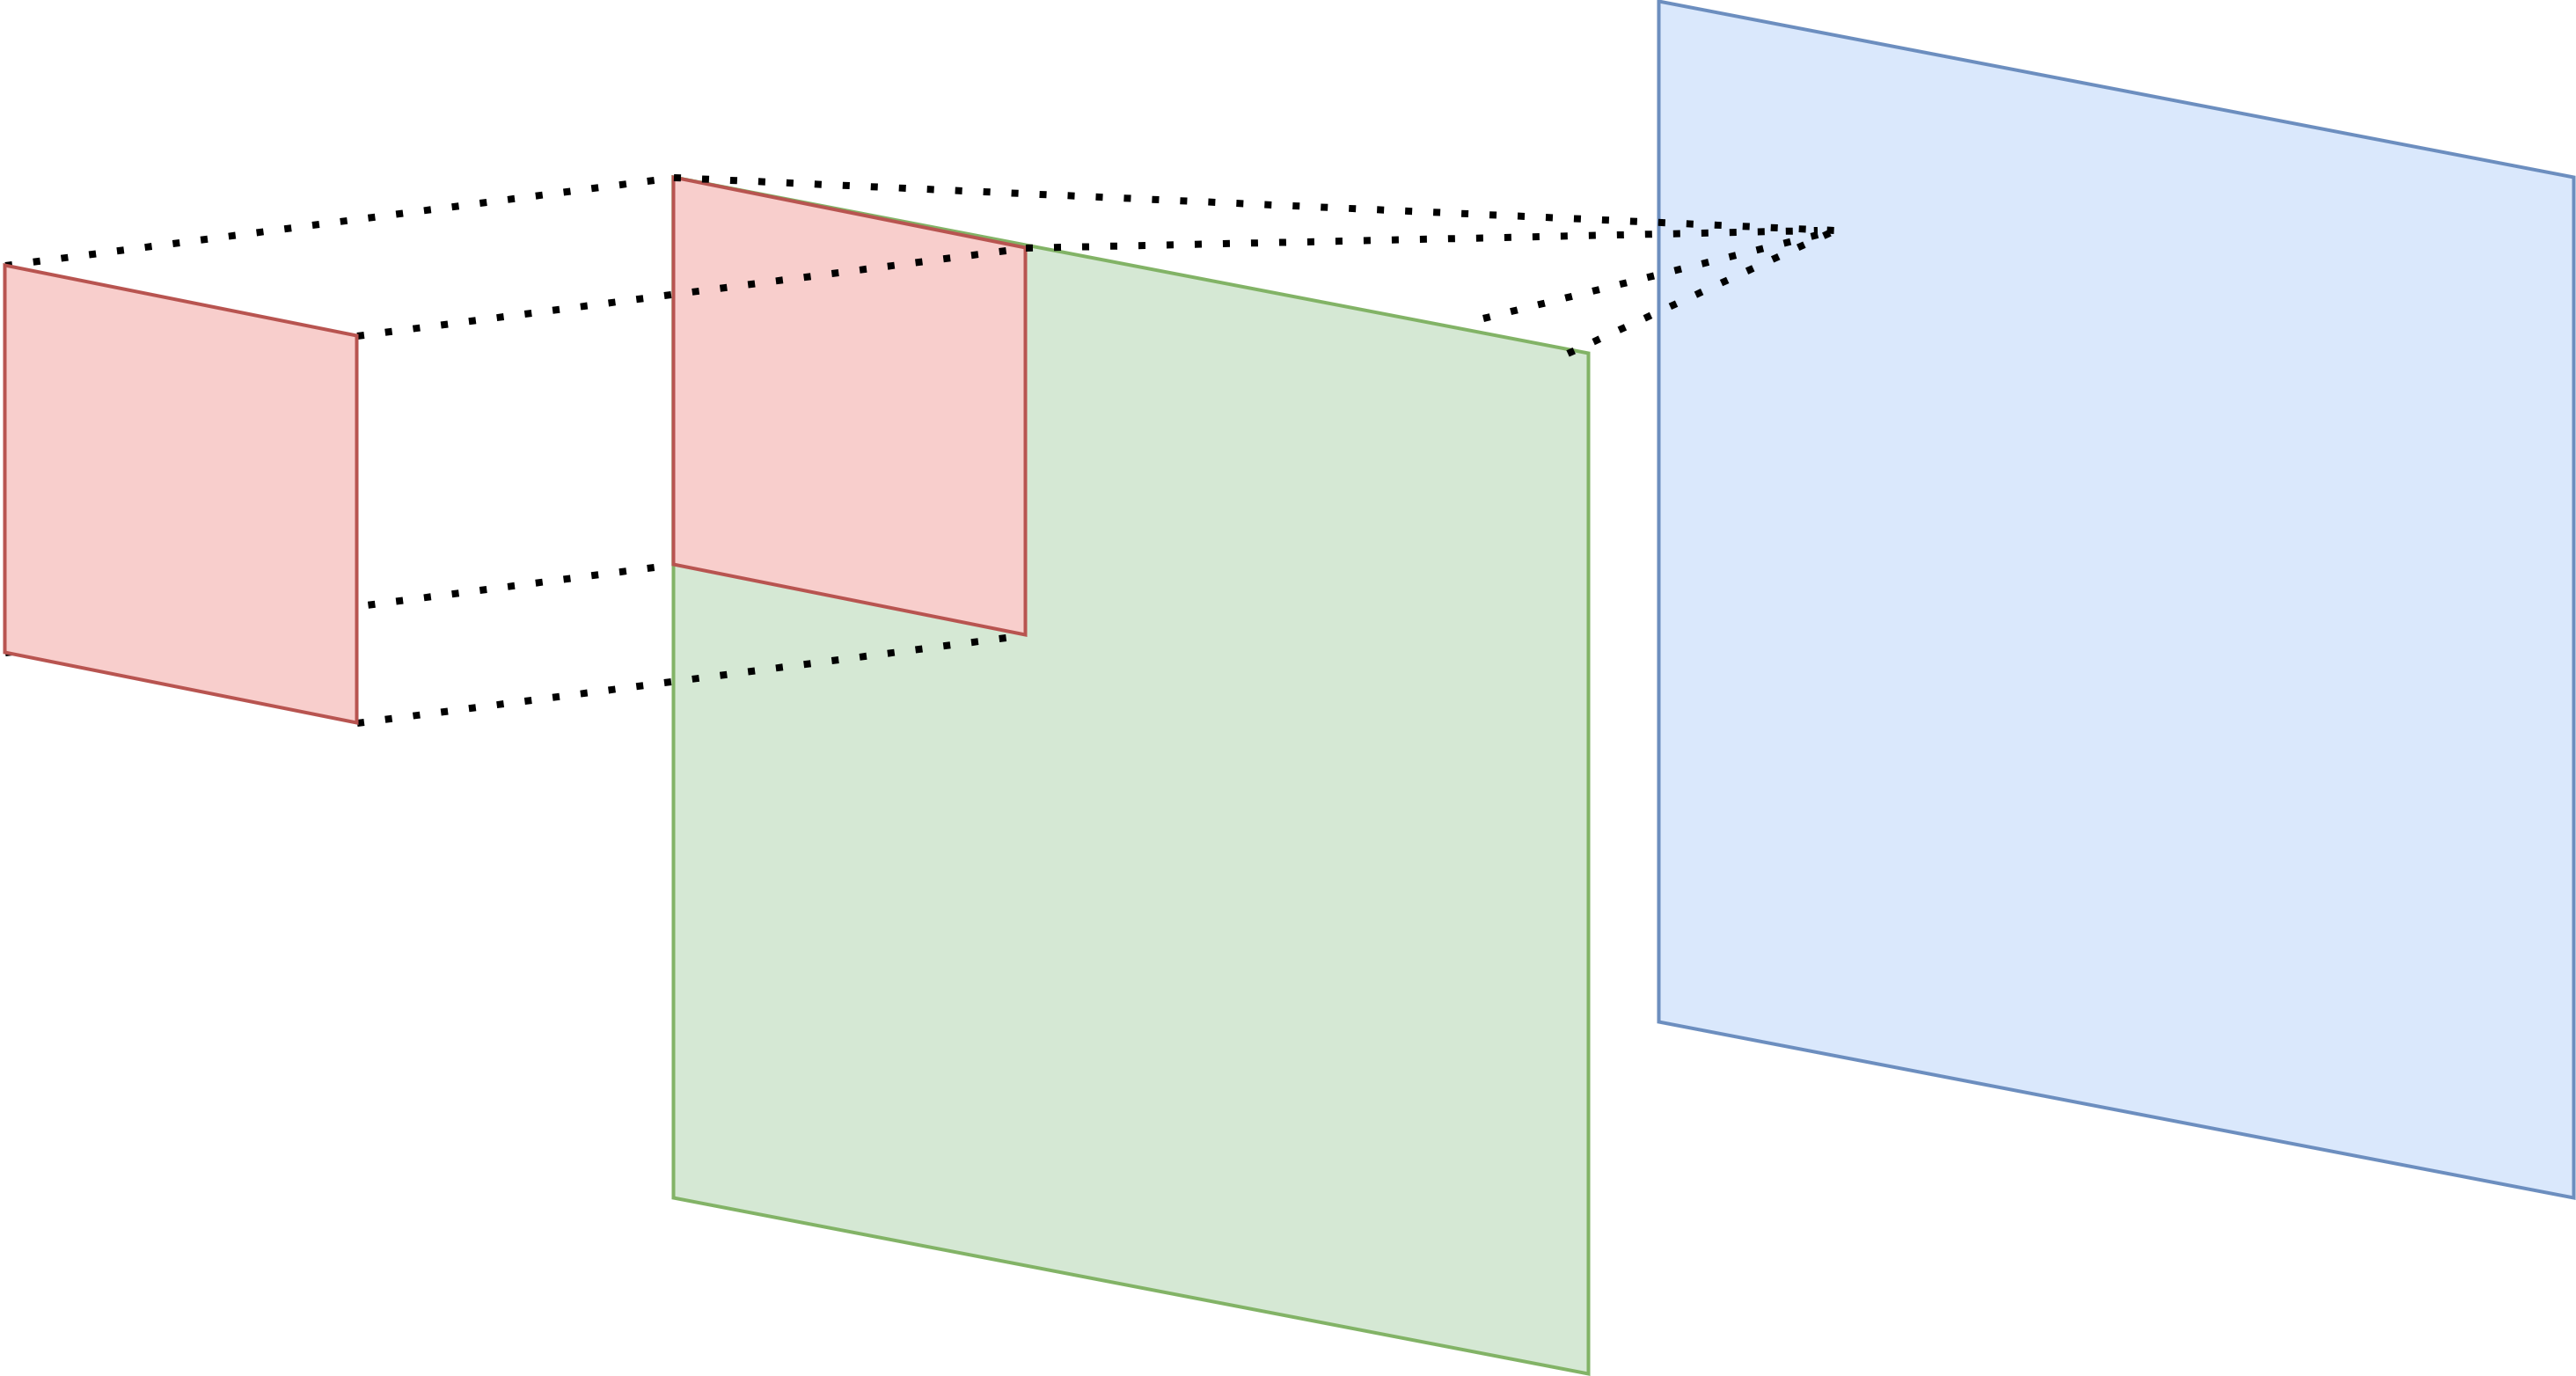
\includegraphics{2_8_convolution_sliding}
  \labfig{2_8}
  \caption[2D Depiction of the Convolution Operation]{
  In the convolution operation the kernel (red square) is applied over the image
  (green square) to produce the corresponding value on the feature map (blue
  square). To compute the next value, the kernel is then slid by a number of positions determined by the \emph{stride}.
  }
\end{marginfigure}
To intuitively comprehend the application of a convolution over a
two-dimensional image, one can visualize it as applying a patch (kernel) of $M
\times N$ elements over the image and computing its weighted sum. This process
involves sliding the patch across all values of the image, with the step size,
known as the \emph{stride}, determining the movement of the kernel to subsequent
positions. In scenarios involving multiple channels, the operation is performed
by applying each patch with identical dimensions to each channel independently
and in parallel. To manage data at the edges of the image, zero padding is
typically applied to the original image, ensuring that the convolution process
can address corner data without loss.

\subsubsection{Pooling Layer}
The pooling prior is encoded by the \emph{pooling layer}. This layer performs a
down-sampling of the input signal, utilizing a sliding window approach similar
to the convolution operation discussed previously. Various down-sampling methods
can be employed, but this discussion focuses on the most commonly implemented
strategies in pooling layers. \refeq{2_20} illustrates the output of an average
pooling neuron and a max-pooling neuron, respectively, applied to an $M \times
N$ window\sidenote{Typical window sizes for pooling layers are $2 \times 2$ and
$3 \times 3$.}.
\begin{equation}
    \labeq{2_20}
    \begin{split}
    P^{avg}(\mathbf{X})_{x, y} &= \frac{1}{L \cdot K} \sum^{L/2}_{l=-L/2}\sum^{K/2}_{k=-K/2} \mathbf{X}_{x - l, y - k}\\
    P^{max}(\mathbf{X})_{x, y} &= \max_{\substack{l \in -L/2, \dots, L/2\\k \in -K/2, \dots, K/2}} \mathbf{X}_{x - l, y - k}
    \end{split}
\end{equation}
Just as the convolution, this process is applied in a sliding window manner. It
follows that the considerations regarding edge handling and striding made
previously are valid for this layer as well. Another important consideration
regarding the pooling layer is that it does not contain any learnable
parameters, which significantly reduces the computational complexity of the
model.

\subsubsection{Network Architecture}
Having discussed the fundamental building blocks of convolutional networks, the
focus now shifts to the actual model architecture, specifically how these blocks
are arranged to construct a model.
Typical convolutional neural network architectures consist of two main
components: a feature extractor and a fully connected head. The feature
extractor comprises a series of convolutional and pooling layers. The rationale
behind this structure is that convolutional layers, through the application of
filters to the input image, generate feature maps that emphasize various image
aspects, such as edges, textures, and complex patterns. Conversely, pooling
layers select the most significant features by down-sampling the input, thereby
reducing the spatial dimensions of the feature maps. The sequential application
of these operations progressively transforms the input data into smaller feature
maps that capture increasingly abstract information about the image\sidenote{
For example, initial convolutional layers might detect simple features such as
edges and corners, while deeper layers might recognize more complex structures
like shapes and objects.}.

The feature extractor is also referred to as the \emph{encoder} because it
encodes the image data into a compact representation containing all the salient
features necessary to solve the task for which the network has been optimized.
Consider, for instance, a CNN that processes input images with three channels
(RGB) and dimensions $W \times H$. Through the progressive application of
convolution and pooling layers, the final feature map (the output of the
encoder) might have dimensions of $8 \times 8$. The output of the model is often
\emph{flattened}, meaning it is reshaped into a one-dimensional vector,
resulting in an output of 64 features. Consequently, the encoder part of the
network can be viewed as a mapping $\mathbb{R}^{W \times H \times 3} \to
\mathbb{R}^{64}$. This 64-dimensional space is called the \emph{latent space}
because the vectors in this space contain \emph{latent} (hidden) features that
the model has learned during training.
\begin{figure}
  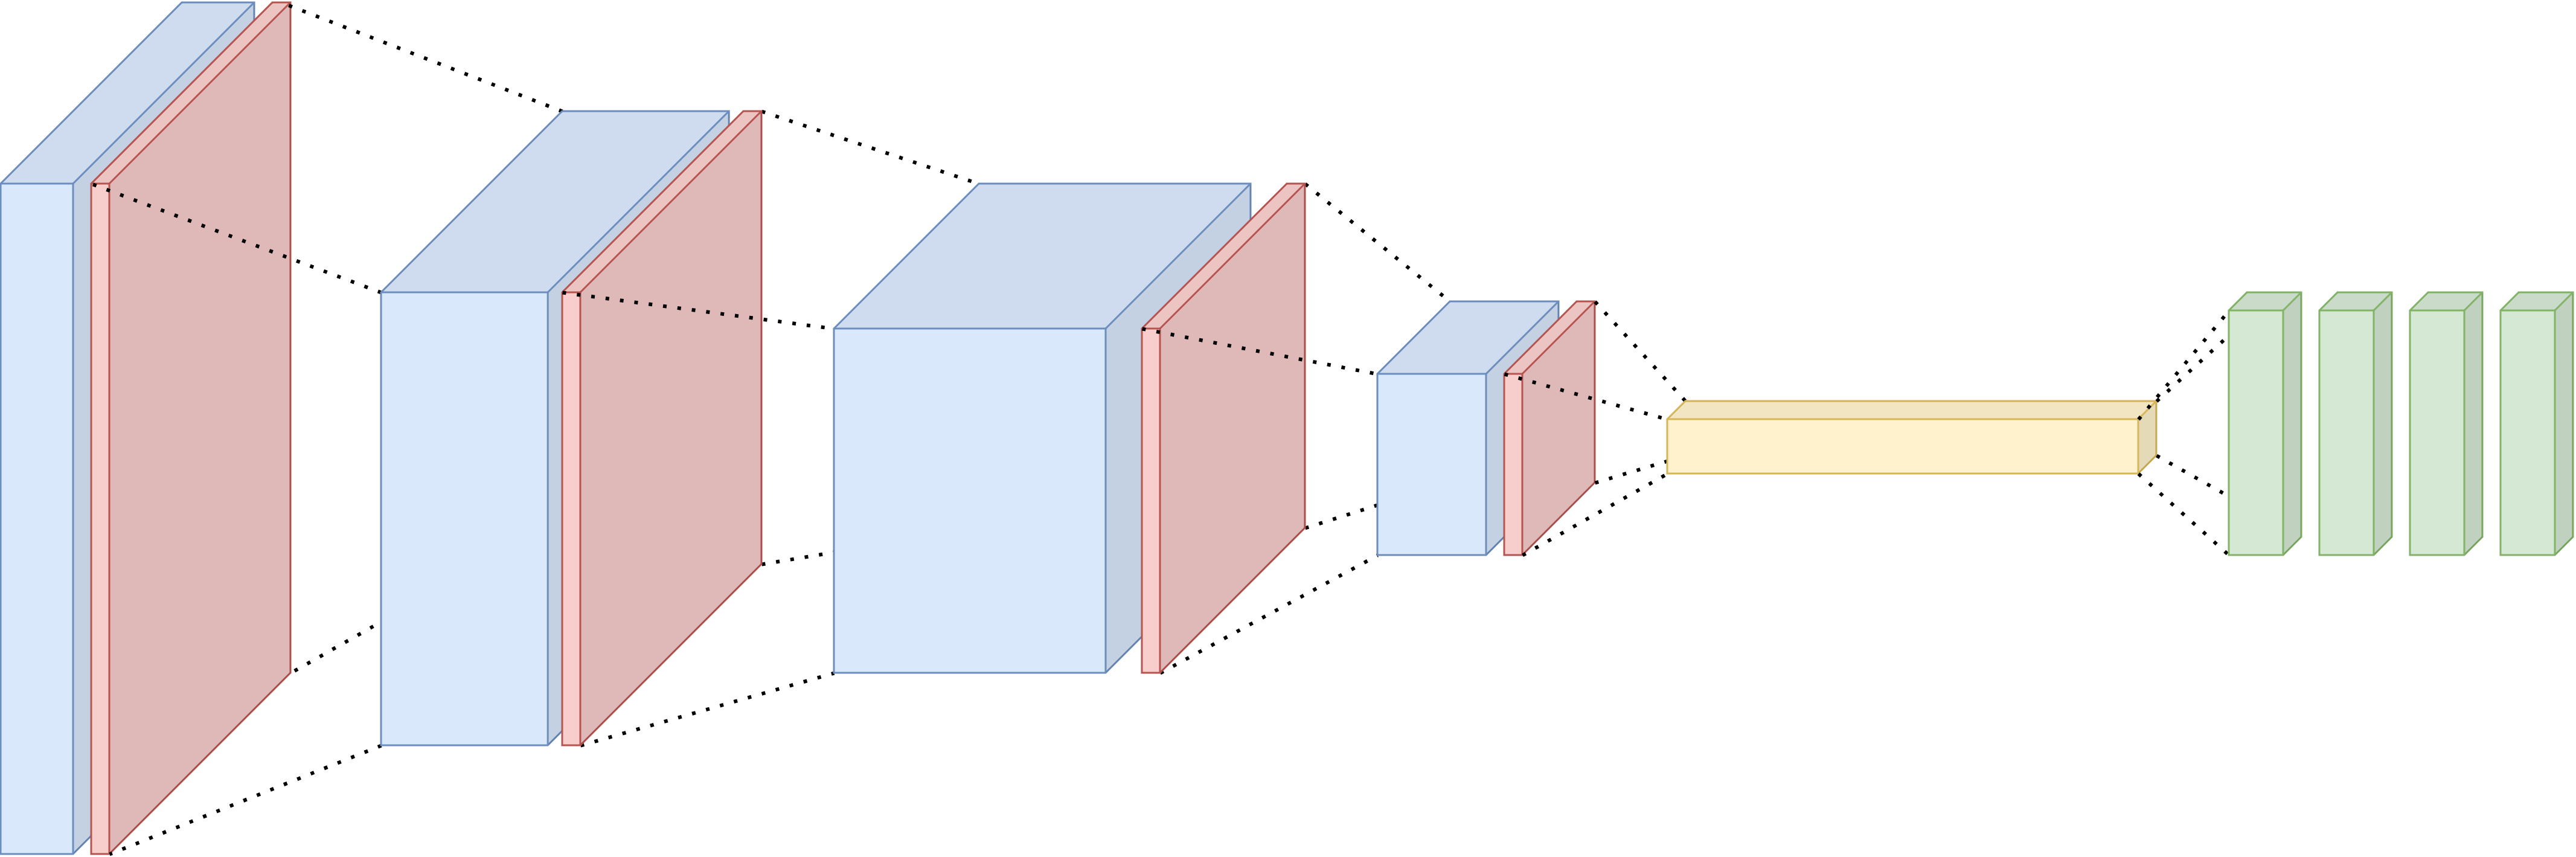
\includegraphics{2_9_convolutional_network}
  \caption[Convolutional Network Architecture]{Graphical depiction of
  Convolutional Neural Network Architecture. In blue are represented
  convolutional layers. Their depth is proportional to the number of filters
  applied in parallel by the layer. In red are depicted the pooling layers,
  while in green the fully connected layers. The yellow block represents the
  hidden representation, that is, the flattened vector that represents the
  encoder's output.}
  \labfig{2_9}
\end{figure}
The encoding part of the model serves to extract all salient features from the
image, progressively selecting them until a compact representation of the input
is obtained. This representation is then fed into the second part of the model:
a fully connected neural network, which performs the actual task, such as image
classification.

Due to the reduced number of parameters in convolutional layers, CNNs can scale
up with a significantly larger number of layers while maintaining manageable
computational complexity. Although all convolutional networks follow a similar
structure, they vary in the number and types of layers, as well as in their
hyper-parameters. Extensive research has been dedicated to identifying the
optimal convolutional network architecture, focusing on the most effective
number and configuration of convolutional, pooling, and fully connected layers.
\reftab{2_3} summarizes some of the most prominent convolutional architectures
found in the literature, along with their total number of parameters.
\begin{margintable} %[ht]
    \resizebox{\textwidth}{!}{
    \begin{tabular}{ l c } \toprule Architecture & Parameters \\ \midrule
        AlexNet \cite{krizhevsky_alexnet_2012} & 60M\\ VGG-16
        \cite{simonyan_vgg_2015} & 138M\\ ResNet18 \cite{he_resnet_2016} &
        11.4M\\
        DenseNet100 \cite{huang_densenet_2018} & 0.8M\\
      \bottomrule
    \end{tabular}
    } 
    \caption[Common Convolutional Network Architectures]{
    Common convolutional network architectures, along with their total number of
    parameters. The architectures are arranged chronologically from older to
    more modern designs. It is noteworthy how the number of parameters has
    decreased over the years, attributed to the development of more efficient
    techniques, which are beyond the scope of this discussion.
    }
    \labtab{2_3}
\end{margintable}
During this work, the ResNet \sidecite{he_resnet_2016} architecture has been
predominantly employed, as will be further discussed in~\refch{anatcl}.
Therefore, it is worth to briefly discus its details here.

\subsubsection{ResNet}
To understand the rationale behind the ResNet architecture, it is crucial to
first comprehend the vanishing gradient problem. As discussed previously,
gradient-based optimization methods function by calculating the gradient of the
loss with respect to the model's parameters. These gradients are computed using
an algorithm that applies the chain rule, multiplying the gradients at each
intermediate computational step. However, a challenge arises when the gradients
from these intermediate steps are small. As these gradients are propagated back
toward the input layers, they can become progressively diminished. This leads to
the vanishing gradient problem, where early layers receive an increasingly
smaller gradient signal, effectively stalling the training of the model as these
layers learn very slowly or not at all. This poses a significant challenge for
the training of deeper networks, as the vanishing gradient problem becomes more
pronounced with an increase in the number of layers\sidenote{This is due to the
proportional increase in the number of dilution steps through which the gradient
must pass.}.
\begin{figure*}
    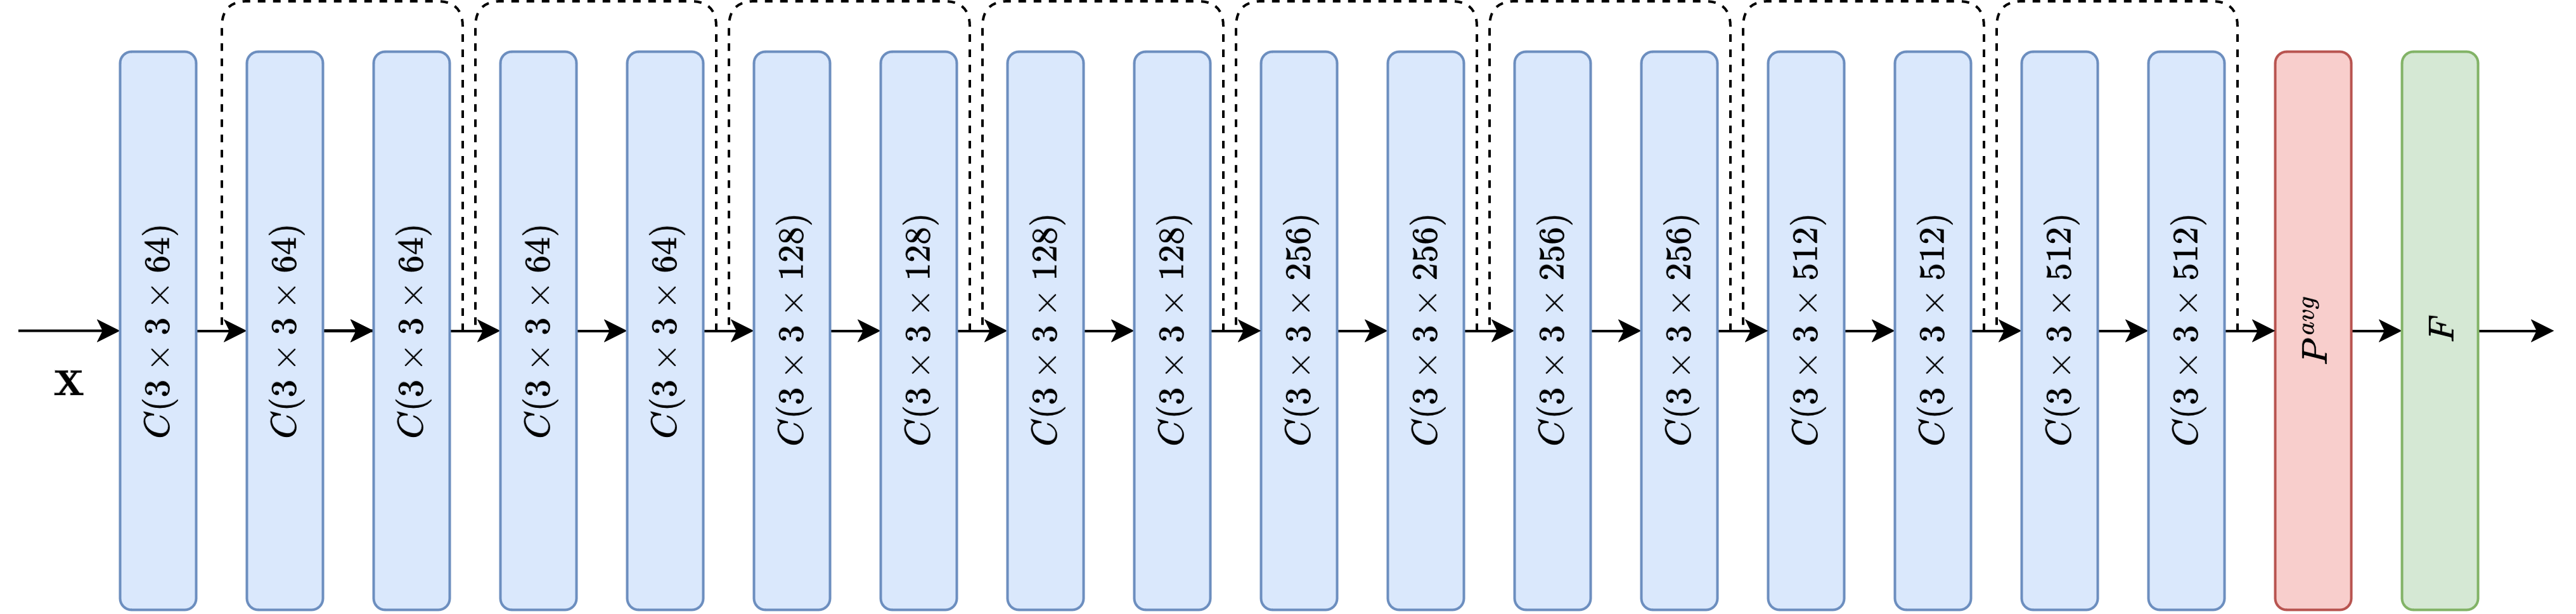
\includegraphics{2_10_resnet_architecture}
    \caption[ResNet-18 Architecture]{Graphical depiction of the ResNet-18
    architecture. The residual connections between layers are depicted in dashed
    lines. Each convolutional block, depicted in blue, is labeled with its
    dimensions $W\times H \times C$, representing width, height, and channel
    count, respectively.}
    \labfig{2_10}
\end{figure*}
However,~\citeauthor{he_resnet_2016}~\cite{he_resnet_2016} demonstrated that
using a special type of connection, known as \emph{residual connections}, can
effectively mitigate this issue. Residual connections allow gradients to flow
directly through the network by skipping layers. By introducing a shortcut path
that bypasses the non-linear transformations, the network can learn identity
functions where necessary, ensuring that the signal is not diluted through deep
layers. This approach has significantly facilitated the training of deeper
networks, as it provides a way for the gradient to pass through without being
dampened by multiple layers of data transformation.
\begin{marginfigure}[*-10]
   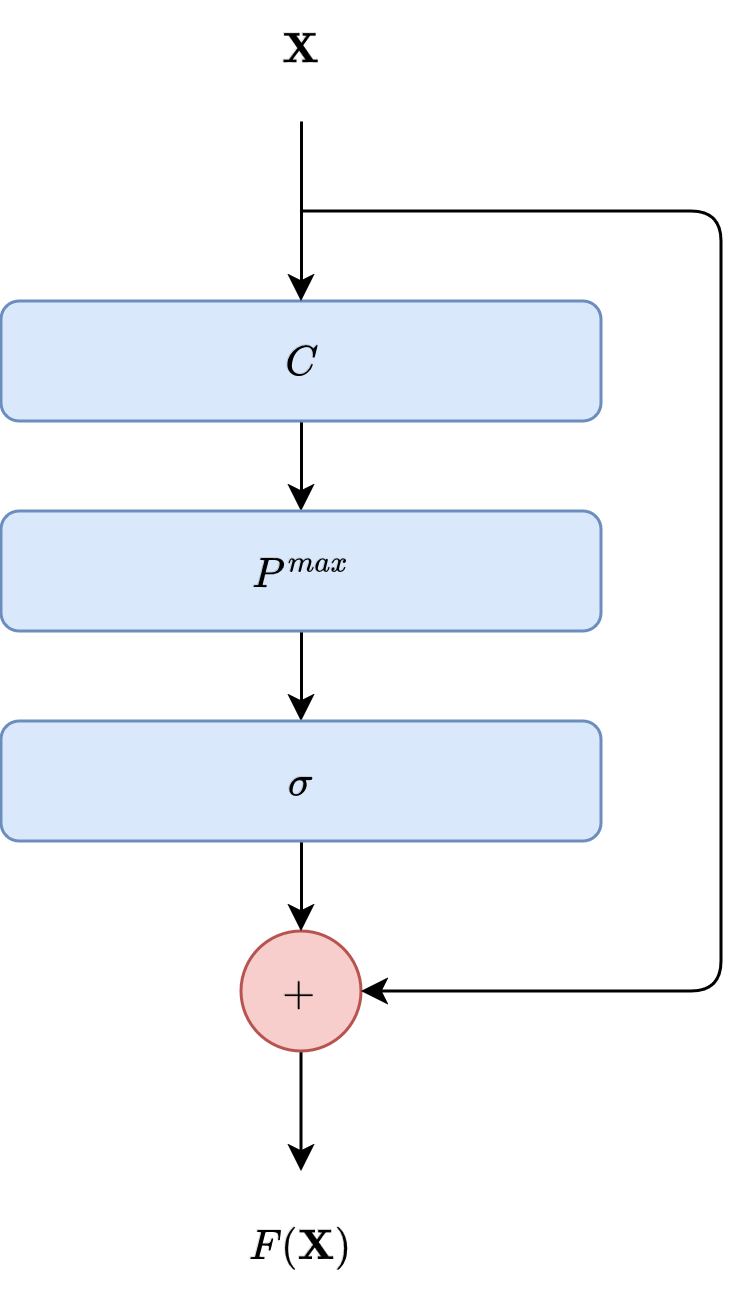
\includegraphics{2_11_residual_block}
   \caption[Residual Block]{A residual block composed of a convolutional layer
   $C$, max pooling layer $P^{max}$ and an activation function $\sigma$. The
   residual connection connects the input $\mathbf{X}$ of the residual block to
   its output $F(\mathbf{X})$ by summing them together. In other words, the
   output of this residual block can be represented as $F(\mathbf{X}) = (C \circ
   P^{max} \circ \sigma)(\mathbf{X}) + \mathbf{X}$.}
\end{marginfigure}
The set of layers that are bypassed by the residual connection is known as a
\emph{residual block}. The skip connection within these blocks is
straightforwardly implemented by summing the input of a residual block to its
output. ResNet incorporates these fundamental units, each comprising
convolutional layers. In the original paper by
\citeauthor{he_resnet_2016}~\cite{he_resnet_2016}, the authors propose different
versions of this architecture, reflecting various sizes and depths. In this
thesis, the primary focus has been on employing the ResNet-18 architecture, a
variant of the ResNet family that consists of 18 layers. This architecture
adheres to the typical design principles of convolutional networks but
incorporates residual connections between layers to enhance learning in deeper
networks. \reffig{2_10} provides a detailed illustration of the ResNet-18
architecture.

\setchapterstyle{kao}
\chapter{Neuroimaging}
\labch{neuroimaging}

Neuroimaging serves as a powerful tool for the non-invasive examination of in
vivo brain structure and function, offering critical insights into brain
operations and the genesis of various conditions. Magnetic Resonance Imaging
(MRI) stands out among diverse imaging techniques for its ability to produce
high-resolution images without employing ionizing radiation, rendering it
invaluable in both clinical settings and research applications. This chapter
provides an overview of the main neuroimaging techniques, with a particular
emphasis on MRI and T1-weighted imaging. The chapter begins by outlining the
principal acquisition methods foundational to neuroimaging, highlighting how
each technique captures unique aspects of brain anatomy and function. The focus
then shifts to the various MRI modalities, with a particular focus on the
characteristics and applications of T1-weighted imaging, which is renowned for
its effectiveness in delineating the brain's anatomical structures. The
discussion then progresses to processing methods typical in neuroimaging,
focusing particularly on Voxel-Based Morphometry (VBM), an advanced analytical
technique that enables detailed structural analysis of the brain through
statistical means. Lastly, this chapter presents brain parcellation techniques
crucial for segmenting the brain into distinct anatomical regions. Particular
attention is given to
the~\citeauthor{desikan_automated_2006}~\cite{desikan_automated_2006} atlas, a
widely utilized parcellation scheme in this thesis.

\section{Acquisition Methods}
In neuroimaging, a variety of acquisition technologies are employed, each
tailored to capture distinct aspects of brain structure and function. Below is a
general overview of several key neuroimaging acquisition techniques:
\begin{itemize}
    \item \textbf{Structural Magnetic Resonance Imaging (sMRI)}: uses magnetic
    fields and radio waves to generate detailed images of the brain. MRI can be
    tailored to highlight various tissue properties and includes several
    specific types that will be discussed further on.
    \item \textbf{Functional Magnetic Resonance Imaging (fMRI)}: uses magnetic
    fields to measure brain activity by means of changes associated with blood.
    flow\sidenote{When an area of the brain is in use, blood flow to that region
    also increases.}. fMRI can be used to observe neural activity and to define
    functional anatomy of the brain.
    \item \textbf{Diffusion Magnetic Resonance Imaging (dMRI)}: leverages the
    magnetic properties of water molecules to map the diffusion of water present
    in the brain's white matter. This acquisition method help in visualizing and
    analyzing the brain's white matter tracts, providing insights into the
    brain's connectivity and structural integrity.
    \item \textbf{Computed Tomography (CT)}: uses X-rays to create detailed
    images of the brain. Particularly useful for quickly detecting injuries,
    bleeding, tumors, and other structural abnormalities.
    \item \textbf{Positron Emission Tomography (PET)}: uses radioactive tracers
    to observe metabolic processes in the brain. PET is highly effective for
    studying brain metabolism and blood flow, and is often used in research on
    neurological and psychiatric conditions.
    \item \textbf{Single Photon Emission Computed Tomography (SPECT)}: similar
    to PET, SPECT uses radioactive tracers and a gamma camera to detect cerebral
    blood flow and brain activity functional changes.
    \item \textbf{Electroencephalography (EEG)}: uses electrodes placed along
    the scalp to detect electrical activity in the brain. EEG is particularly
    valuable for diagnosing conditions like epilepsy and sleep disorders, and
    for research on brain states such as alertness or sleep.
    \item \textbf{Magnetoencephalography (MEG)}: records magnetic fields
    produced by neural activity, offering a direct measurement of brain
    activity. MEG is used to study cognitive functions, neural responses, and to
    map brain functions.
\end{itemize}

It's important to note that this list of neuroimaging acquisition technologies
is not exhaustive. There are additional methods and variations within each
category that may be used depending on specific diagnostic or research needs.
Each technology offers distinct advantages for exploring different facets of
brain structure and function, but it is beyond the scope of this work to discuss
all of them in detail. This thesis will specifically focus on Deep Learning
techniques applied to Magnetic Resonance Imaging (MRI), and thus the discussion
will now shift to this neuroimaging modality in particular.

\section{Magnetic Resonance Imaging (MRI)}
An MRI scanner primarily functions as a large magnet that creates a constant
magnetic field strength ($B_0$) when activated~\sidecite{grover_mri_2015}.
During an MRI scan, a patient is positioned within the scanner's bore, and the
hydrogen protons ($H_1$) within the patient's body are exposed to this static
magnetic field. This exposure causes the protons' spins to
precess\sidenote{Precession is a change in the orientation of the rotational
axis of a rotating body.} around the $B_0$ direction. To manipulate these spins,
Radiofrequency (RF) excitation pulses are directed to the head or a specific
body section through either a single transmission coil or an array of them.
These RF pulses align the proton spins within the targeted area to the direction
of the RF pulses.

Once the RF pulses cease, the aligned spins begin to relax back to their initial
states. This relaxation process varies based on the surrounding environment and
the magnetic resonance (MR) relaxation properties of different tissue types
within the body. The energy released during this relaxation is captured by one
or more receiver coils, translating it into a raw data matrix known as
\emph{k-space}. As a final step, this data undergoes a series of
signal-processing techniques that transforms this raw data into the MR images
that are then used for clinical assessment or research.
\begin{figure}
    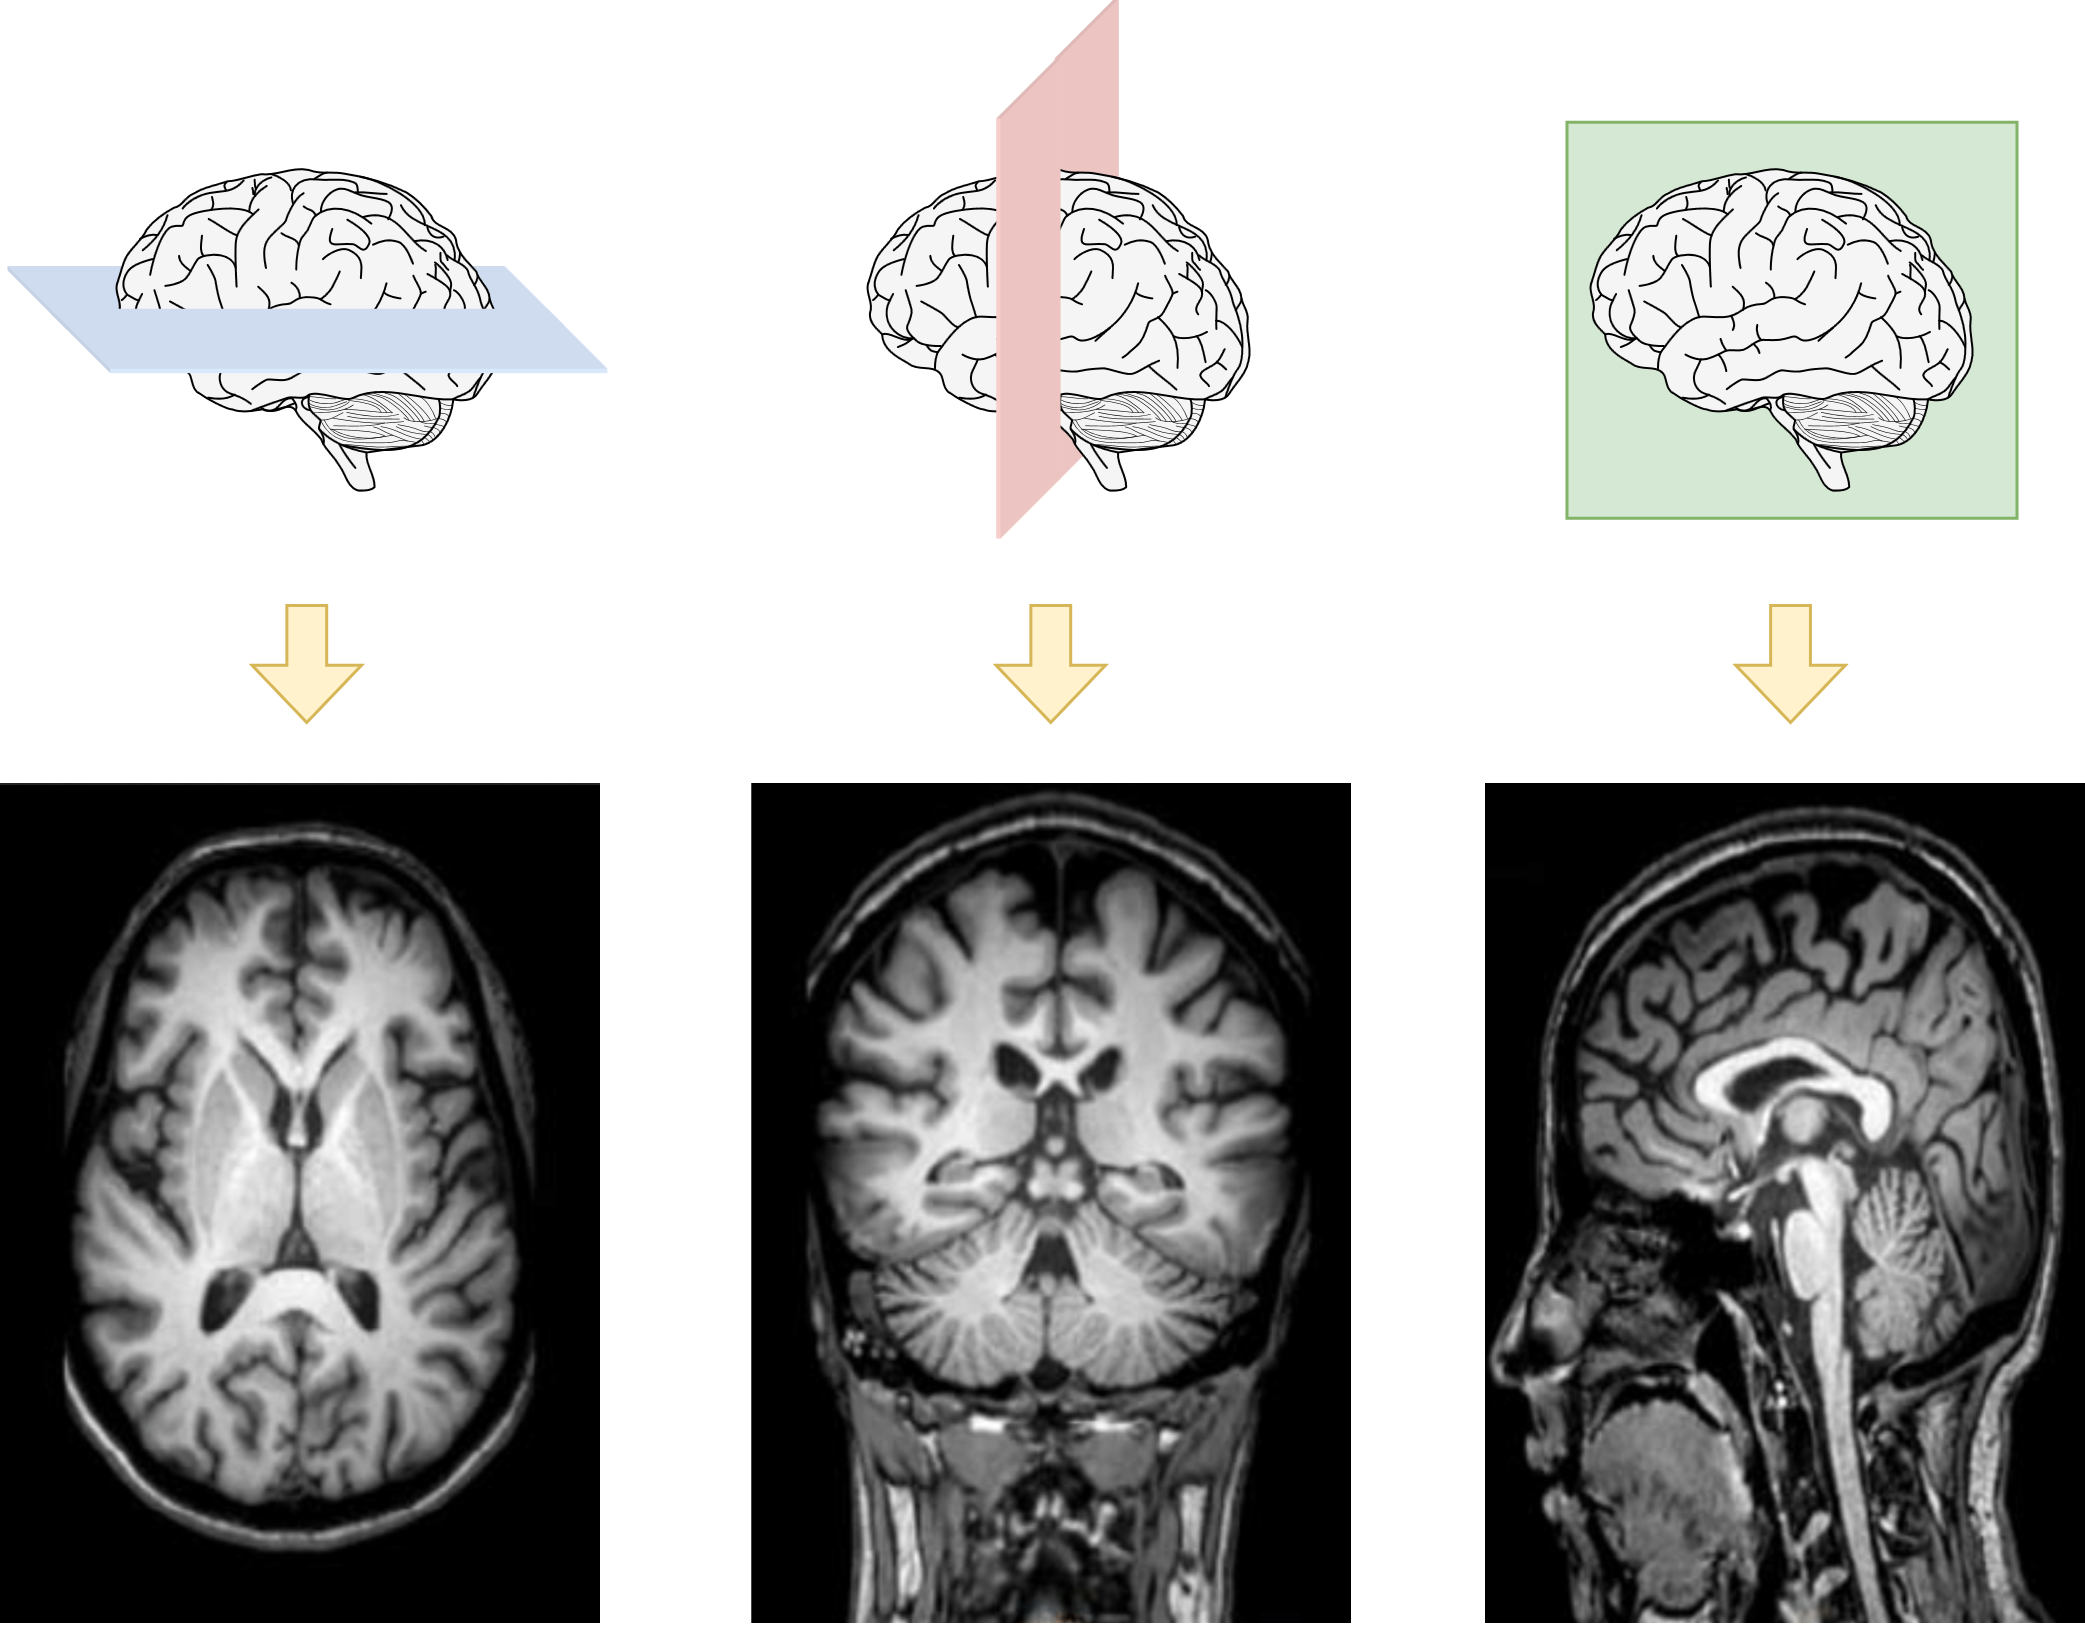
\includegraphics{3_1_acquisition_planes}
    \caption[Acquisiton Planes of an MRI Scan]{An MRI scan captures images of the brain from three different
    planes: axial, coronal, and sagittal. This figure shows the acquisition
    planes along with their corresponding generated images. The axial plane is
    depicted in blue, the coronal plane in red, and the sagittal plane in green.
    }
    \labfig{3_1}
\end{figure}
MR images are composed of digital image voxels, which are essentially 3D
volumes, in contrast to pixels that represent 2D squares. Each voxel in an MR
image contains a signal that represents all the MR-visible protons within that
specific volume. This setup allows for a three-dimensional representation of the
scanned area, providing depth that a two-dimensional pixel-based image cannot.

Higher magnetic field strengths in MR scanners enhance the quality of these
images. The stronger the magnetic field ($B_0$), the greater the level of detail
that can be achieved. This is because higher field strengths improve the
signal-to-noise ratio and the resolution of the images, allowing for better
differentiation of tissue types and more precise imaging of fine structures.
Consequently, MR scanners with higher field strengths are capable of producing
images with better clarity and more distinct separation of
signals\sidenote{For instance, MRI scanners commonly found in hospitals utilize
magnetic field strengths of either 1.5 Tesla or 3 Tesla.}

As mentioned earlier, each tissue type responds uniquely to the magnetic pulses
used in MR imaging. This differential response is precisely what the so called
T1 and T2 weighting exploit to enhance the visibility of various tissues within
the magnetic resonance images.
\begin{marginfigure}
    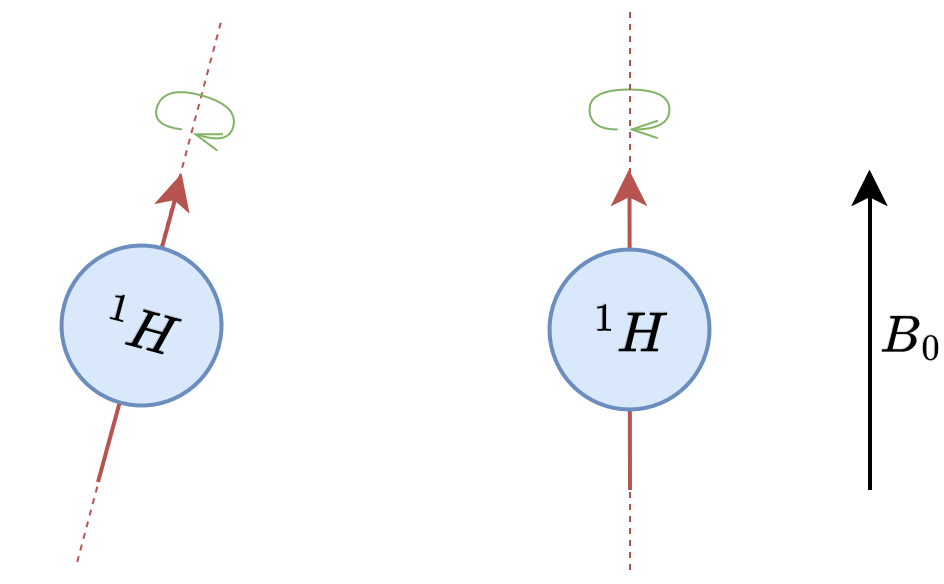
\includegraphics{3_2_spin_hydrogen}
    \caption[Spin of an Hydrogen Atom]{Hydrogen atoms spin along their axis.
    When a magnetic force is applied ($B_0$) their rotational axis is pulled
    towards the direction of the magnetic field.}
    \labfig{3_2}
\end{marginfigure}
T1-weighted imaging capitalizes on the \emph{longitudinal relaxation time}
($T_1$), which is the time it takes for protons to realign with the magnetic
field $B_0$ after the removal of the RF pulse. T1 times vary between different
types of tissue; for instance, fat has a shorter T1 time compared to water. In
T1-weighted images, tissues with shorter T1 relaxation times appear brighter.
Thus, these images are particularly effective for visualizing the anatomy of the
brain, distinguishing between grey and white matter, and identifying fatty
tissues, making them valuable for detailed anatomical studies.

T2-weighted imaging, on the other hand, emphasizes the \emph{transverse
relaxation time} ($T_2$), which is the time it takes for protons to lose phase
coherence among the directions perpendicular to the magnetic field, primarily
due to interactions with neighboring molecules. Tissues with longer T2 times,
such as fluids, appear brighter on T2-weighted images. This characteristic makes
T2-weighted imaging exceptionally useful for detecting fluid-filled areas, such
as edema, tumors, and inflammation in tissues.

The choice between T1 and T2 weighting depends on the diagnostic requirements;
T1 is preferred for detailed anatomical definition, while T2 is superior for
identifying fluid changes. This flexibility is a key strength of MRI technology,
allowing for tailored imaging that aligns closely with clinical and research
needs. In this work, the datasets used contained predominantly T1-weighted
images. 

\section{Voxel Based Morphometry}
Following the acquisition phase, MRI images can undergo analysis either
automatically (e.g., by a machine learning model) or manually. Nonetheless,
several inherent challenges may compromise the reliability of the data,
especially when comparing images across different individuals. Each individual's
brain presents distinct anatomical characteristics, including variations in
size, shape, and the distribution of tissues such as gray matter (GM), white
matter (WM), and cerebrospinal fluid (CSF). These discrepancies complicate
direct comparisons between scans because corresponding brain regions may not
align precisely across different individuals. This variability also impedes the
ability to draw comparisons or discern trends across populations or patient
groups\sidenote{Coincidently, a task that must be performed by Neural
Networks.}. Additionally, MRI scans are prone to various types of noise and
artifacts, which may originate from the scanner, environmental conditions, or
subject-related factors such as minor movements during scanning. These
extraneous signals can mask essential details critical for precise diagnosis or
effective research analysis.

To address these challenges, a pre-processing technique called Voxel-Based
Morphometry (VBM)~\sidecite{ashburner_vbm_2000} has been developed. VBM
standardizes and simplifies the process of comparing brain anatomy across
different individuals by focusing on measuring differences in the composition of
brain tissue, specifically the concentration and volume of gray and white
matter. The concept of VBM comprises three basic preprocessing steps: (1)
\emph{spatial normalization}, (2) \emph{tissue segmentation} , and (3)
\emph{spatial smoothing}, which are followed by the actual statistical analysis.

In the spatial normalization step, the MRI scans are matched together spatially
(registered) so that a location in one subject's MRI corresponds to the same
location in another subject's MRI. It is generally achieved by registering all
images from a study onto the same template image\sidenote[][*-4]{A common template
frequently used in the literature is the MNI (Montreal Neurological Institute)
template~\cite{evans_mni_1993}, which has also been utilized in this study.}
so that they are all in the same space. The template image could be one specific
MRI scan or could be created by averaging across a number of different MRI scans
that have been put in the same space.  After the template image has been
obtained, either linear or non linear transformations can be used to perform
this registration~\sidecite{kurth_vbm_2015}. 

The tissue segmentation process is the subsequent step, which involves
partitioning the MRI images into different tissue compartments such as white
matter (WM), gray matter (GM), and cerebrospinal fluid (CSF). As previously
discussed, in T1-weighted images (which are the focus of this thesis) the
longitudinal relaxation time ($T_1$) varies across different types of tissue.
Consequently, each tissue type displays a distinct level of brightness in the
images. This difference allows for the assignment of specific tissue types based
on their brightness levels. Essentially, this phase involves creating a map of
brightness values that correspond to different tissue types, enabling the
accurate identification of each tissue within the MRI images.
\begin{figure*}
    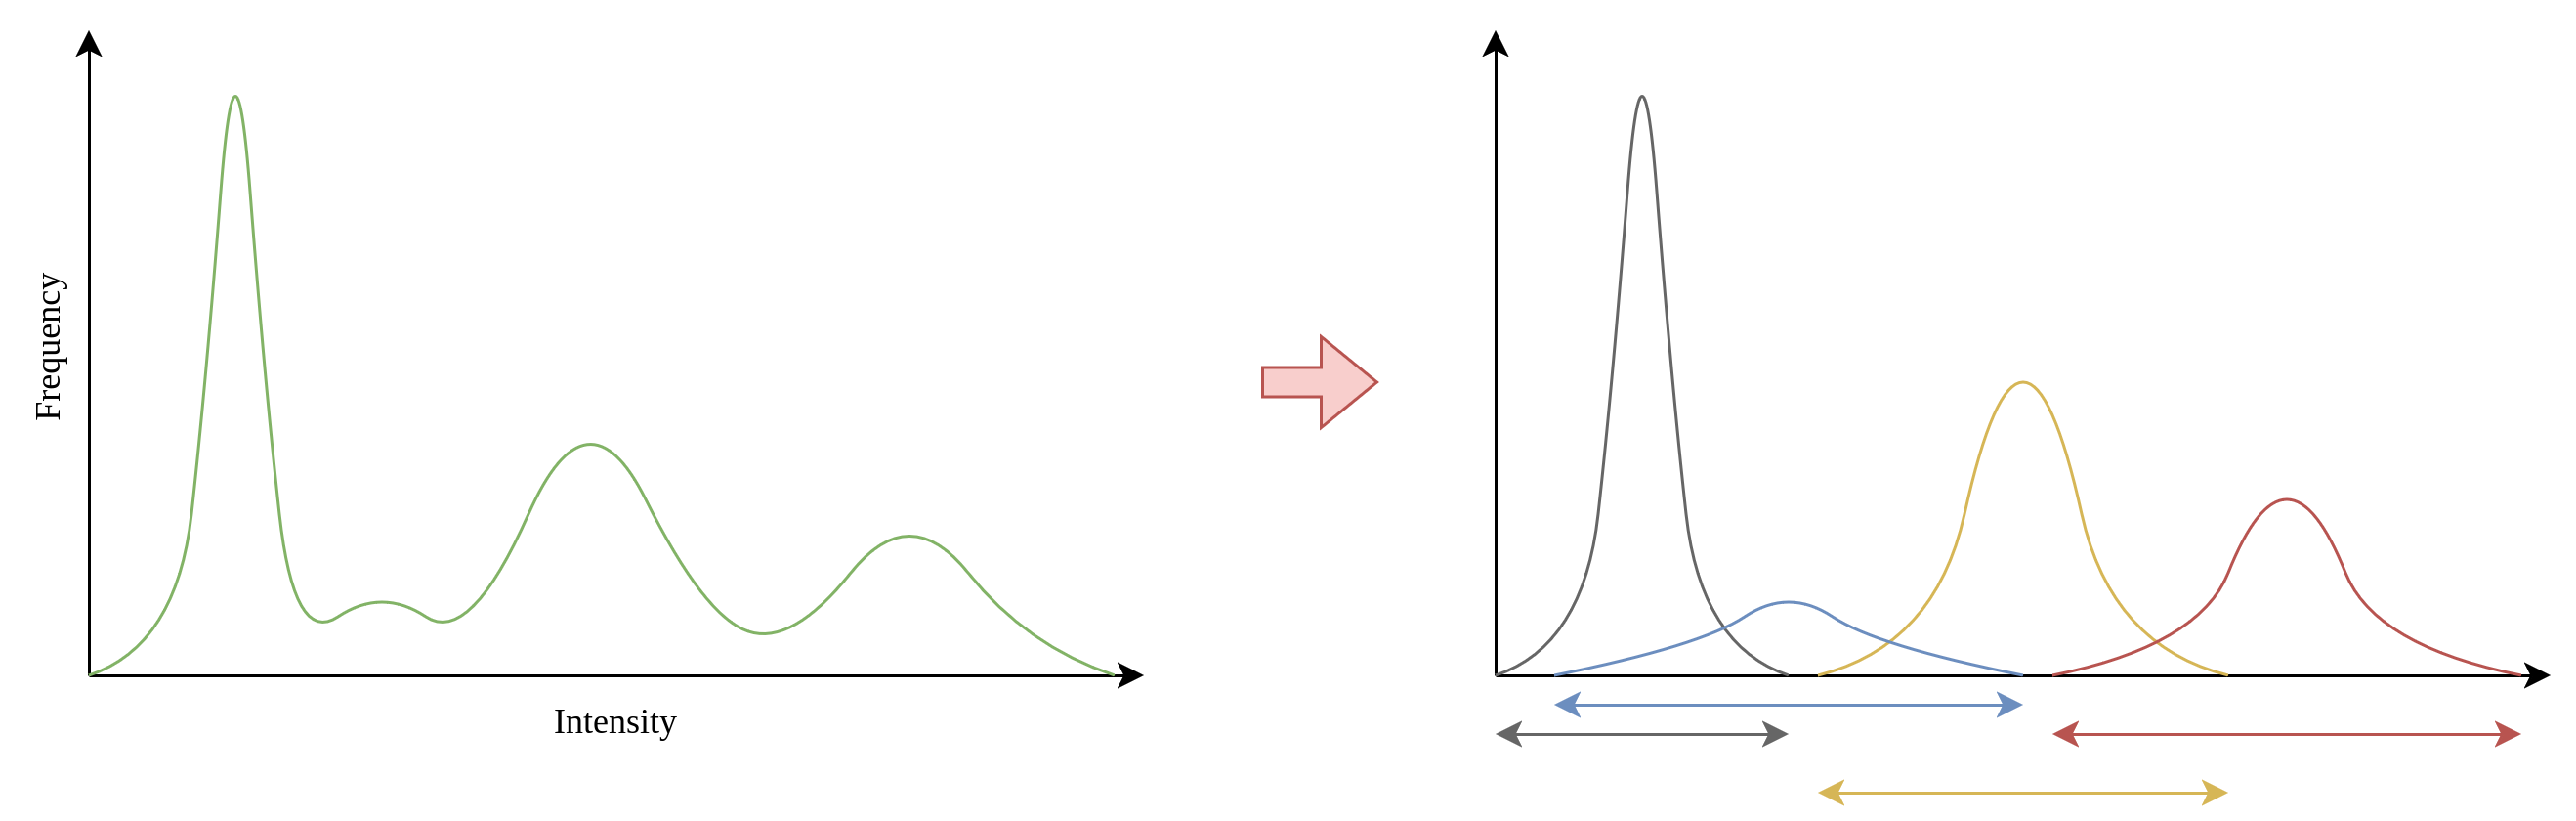
\includegraphics{3_3_segmentation_distribution}
    \caption[Segmentation (Values Distribution)]{On the left, an hypothetical
    distribution of intensity values of an MRI image. When this image undergoes
    tissue segmentation, the original distribution of intensity values is
    segmented into different distributions that represent a specific tissue
    class (right figure). For example, the gray one may represent background,
    the blue cerebrospinal fluid, the yellow white matter and the red grey
    matter. Note that in this case tissue-specific intensity distributions
    overlap. This is due to the fact that each voxel can contain more than one
    tissue.}
    \labfig{3_3}
\end{figure*}
To construct such a map, the distribution of intensity values within the MRI
images is divided into several smaller distributions, each representing a
specific tissue class. In practice, each voxel, commonly measuring $1mm$ isotropic, may contain multiple tissue types, causing overlaps
between the intensity distributions of different tissue classes. This overlap
can result in voxels being classified under more than one tissue category.

To address this challenge, tissue segmentation can be enhanced with the use of
additional probability maps that incorporate prior knowledge about the typical
locations of different tissues within the
brain~\sidecite{ashburner_segmentation_2005}. For each tissue type, a
probability map is used that indicates how likely a particular voxel is to
represent that tissue. This probabilistic approach helps to refine the decisions
made by the tissue classification algorithm, ensuring a more accurate
segmentation. Since the algorithm uses a probabilistic approach, the result is
an estimation of tissue composition for each voxel in the image.

The third and last step consist of a spatial smoothing, which consist on the
application of a convolution operation with a Gaussian filter\sidenote{A
Gaussian Filter is a kernel whose values are sampled from a Gaussian
distribution. In this case, they are sampled from a 3-dimensional Gaussian
distribution.}. The first is that smoothing can improve effectively the
signal-to-noise ratio by averaging the intensities of neighboring voxels. This
reduction in noise is essential because it helps to reveal the true anatomical
differences underlying the images, minimizing the impact of random fluctuations
that might otherwise be mistaken for significant variations.

Moreover, smoothing serves to increase the statistical power of the analyses
conducted in VBM. By making the data more normally distributed across voxels,
smoothing aligns with the statistical assumptions required for many of the
inferential techniques used in neuroimaging studies. This alignment is crucial
as it not only validates the use of parametric statistical tests but also
enhances the reliability of the findings by increasing the effective sample size
at each voxel. This approach provides a more robust basis for detecting
differences that are statistically significant rather than those arising from
the noise.
\begin{figure*}
    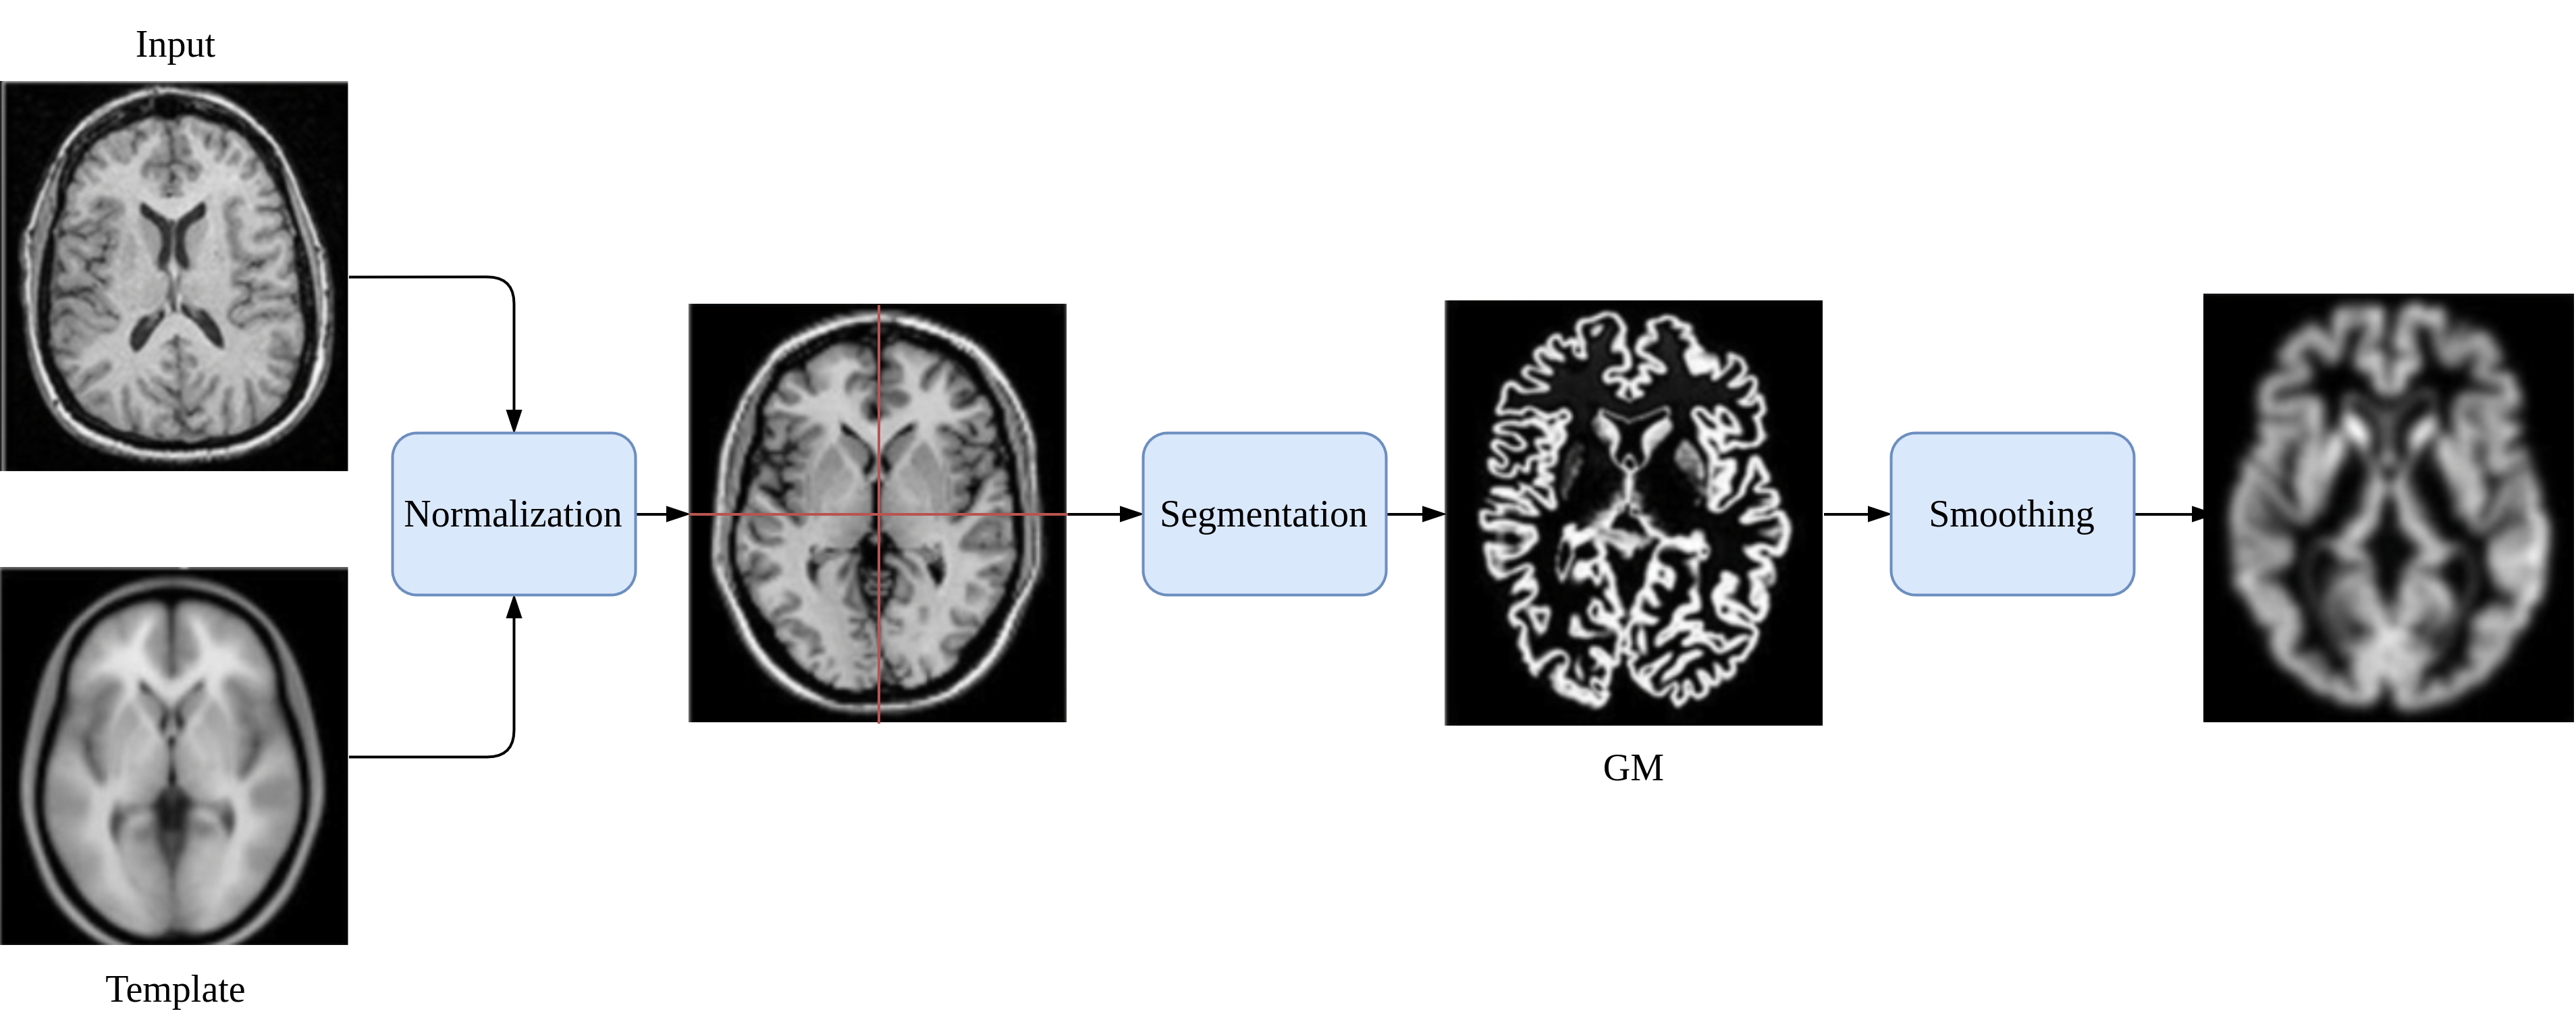
\includegraphics{3_4_vbm_steps}
    \caption[Voxel Based Morphometry Steps]{VBM processing is conducted in three
    steps. Initially, normalization is applied to all images using a standard
    template to ensure that they are aligned to the same frame of reference. The
    second step involves segmenting the normalized images into different tissue
    types, identifiable by their distinct intensity values. This segmentation
    results in the creation of separate volumes for each tissue type; for
    illustrative simplicity, only Gray Matter is depicted in this figure. The
    final step in the VBM process is the application of Gaussian smoothing to
    each of these segmented volumes.}
    \labfig{3_4}
\end{figure*}
Another key aspect of smoothing is its ability to account for minor registration
errors between subjects' images. Despite the application of the spatial
normalization step, slight misalignments can still occur due to the inherent
variability in brain anatomy among individuals. Smoothing helps to mitigate
these differences by blurring sharp edges and increasing the overlap of similar
anatomical structures across different scans. This adjustment is particularly
beneficial for ensuring accurate comparisons are made in studies comparing
groups of subjects, as it helps ensure that equivalent anatomical regions are
analyzed across all images.

Furthermore, smoothing is instrumental in matching the voxel-wise data to the
assumptions of Gaussian field theory, which underpins many of the statistical
methods used to draw inferences from neuroimaging data. This theory relies on
the smoothness of the data to make valid statistical claims about the presence
of significant brain regions. By applying a Gaussian filter, the data better
approximate a continuous Gaussian field, thus fulfilling the theoretical
prerequisites necessary for accurate \emph{p-value} calculation and hypothesis
testing.

Today there are various tools that perform VBM pre-processing, each with its own
choice for the implementations of the aforementioned steps. For the
pre-processing of MRI images used in this work, the
BrainPrep~\cite{grigis_brainprep_2022} software has been used, which is based on
two common pre-processing packages in neuroimaging CAT12~\cite{gaser_cat_2022}
and FreeSurfer~\cite{fischl_freesurfer_2012}.


\section{Brain Parcellations}
Brain parcellation is a method utilized in neuroimaging to divide the brain into
distinct regions based on anatomical landmarks, functional specialization, or
connectivity patterns. This technique is crucial for reducing the complexity of
the brain's architecture into manageable segments, thereby enabling more focused
and detailed analyses of its structure and function. Particularly in anatomical
MRI, parcellation proves invaluable for isolating specific areas of interest to
evaluate their individual contributions to overall brain anatomy.
\marginnote{The terms \emph{parcellation}, \emph{atlas}, and \emph{template} are
often used interchangeably in the literature.}The significance of brain
parcellation stems from its ability to enhance understanding of the
relationships and interactions among various parts of the brain. Segmenting the
brain into regions allows to effectively correlate specific structural changes
with cognitive functions or pathological states, facilitating deeper insights
into brain functionality and disorder.

Brain parcellations not only provide insights into the organizational principles
of the human brain but also offer significant practical benefits as biologically
informed strategies for data reduction. This process allows the information from
hundreds of thousands of voxels in MRI images to be compressed into a manageable
set of regions that reflect distinct
entities~\sidecite{eickhoff_parcellations_2018}. Such reduction is crucial,
particularly for neural network models, which can utilize this streamlined data
to predict behavioral or clinical phenotypes from brain imaging data. However,
for this aggregation to serve as a valid form of data compression, the
delineated parcels must represent a biologically meaningful patterning.

Over the past two decades, a variety of reliable brain parcellations have been
developed, each exhibiting specific strengths and weaknesses. These
parcellations have become essential tools for the analysis of neuroimaging
datasets. Depending on the type of data they utilize, and consequently the
acquisition method employed, these methods can be classified into three broad
categories~\sidecite{moghimi_parcellations_2021}:
\begin{itemize}
    \item Anatomical parcellations, which are constructed from T1-weighted MRI
    images.
    \item Functional parcellations, derived from from functional MRI (fMRI)
    images.
    \item Structural parcellations, based on diffusion-weighted-imaging
    data.
\end{itemize}
This thesis will specifically focus on anatomical parcellations. Within this
context, each defined region, known as a \emph{Region of Interest (ROI)}, is
assigned a specific label. As noted earlier, T1-weighted MRI images effectively
capture the anatomical structure of the brain. This includes the intricate
folding patterns of the cortical surface (its \emph{sulci} and
\emph{gyri}\sidenote[][*-4]{The cortical surface is the outer layer of neural
tissue of the brain. Sulci and gyri are the characteristic folds and ridges of
the brain, respectively.}) as well as sub-cortical structures\sidenote{Unlike
cortical structures, sub-cortical structures are anatomical features located
beneath the cortical surface.}.

A prevalent method for constructing anatomical parcellations involves using gyri
and sulci as markers to delineate the boundaries of regions of interest. The
brain displays prominent sulci that typically demarcate each functional area,
and by examining these major sulci, one can determine the boundaries of each
ROI. The process for identifying the landmarks used to define each ROI, along
with the number of ROIs, is encapsulated in a set of guidelines utilized by
neuroanatomy experts to manually label the MRI images. 

Given a specific set of guidelines, there are multiple methods for parcellating
new brain images. The approach discussed later in this thesis primarily involves
registering a new brain image to a template image that has already been manually
parcellated; this template is referred to as the \emph{reference atlas}.
Typically, a reference atlas is constructed from a collection of brain images
that have been manually segmented according to established guidelines. Once the
reference atlas is prepared, it facilitates the automatic parcellation of new
images.

Each atlas proposed in the literature adheres to a specific set of guidelines,
which results in variations in the number and delineation of Regions of Interest
(ROIs). This thesis will focus on two major atlases: the Desikan-Killiany
Atlas~\cite{desikan_automated_2006}, which has been predominantly utilized in
this research, and the Destrieux Atlas~\sidecite{destrieux_parcellation_2010}.
These atlases exemplify how differing guidelines can influence the definition
and segmentation of brain regions, impacting the analysis and interpretation of
neuroimaging data.

\subsection{Desikan-Killiany}
The Desikan-Killiany parcellation scheme divides the cortical area of the brain
into 34 regions of interest per hemisphere, resulting in a total of 68 ROIs for
the entire brain. To develop the Desikan atlas, the authors utilized a dataset
of 40 MRI scans that had been manually labeled by neuroanatomy experts. Various
sources of information were utilized to delineate the number of ROIs and their
anatomical boundaries, wich are discussed extensively in the original
publication~\cite{desikan_automated_2006} and are beyond the scope of this
discussion.

An automated algorithm, guided by the reference atlas, can
subsequently be applied to each new MRI scan to generate its corresponding
parcellation. In their foundational study, the authors compared a series of
automatically parcellated brains with manually parcellated counterparts. The
results demonstrated sufficient precision to affirm the method's anatomical
validity and reliability, indicating that this automated approach is both
effective and dependable for replicating established neuroanatomical
segmentations.

\begin{figure}
    \begin{subfigure}[h]{.5\linewidth}
        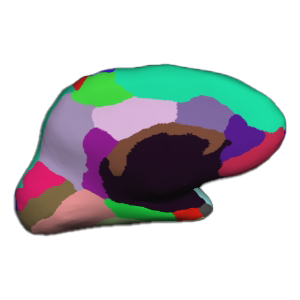
\includegraphics[width=1\linewidth]{3_5_a_desikan}
    \end{subfigure}%
    \begin{subfigure}[h]{0.5\linewidth}
        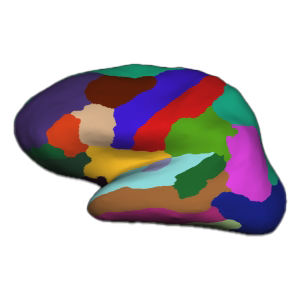
\includegraphics[width=1\linewidth]{3_5_b_desikan}
    \end{subfigure}
    \caption[Desikan Atlas]{Desikan Atlas. Each different color corresponds to a
    specific region of interest.}
\end{figure}

Each ROI within the Desikan scheme is characterized by a vector of different
anatomical measures, calculated over the corresponding volume represented by the
ROI. The selection of features depends on the image analysis software employed.
In this instance, the analysis software
utilized~\sidecite{fischl_freesurfer_2012} encompasses seven anatomical
measures. These measures provide a summary of various structural aspects of the
brain regions, which include:
\begin{itemize}
    \item \textbf{Average Cortical Thickness}: measures the average thickness of
    the cerebral cortex across the corresponding ROI.
    \item \textbf{Standard Deviation of Cortical Thickness}: measures the
    variability in terms of standard deviation of the cortical thickness within
    the ROI.
    \item \textbf{Gray Matter Volume}: quantifies the total volume of gray
    matter within the specified parcellated region.
    \item \textbf{Total Surface Area}: calculates the overall area of the
    cortical surface within each segmented region, relating to the extent of
    cortical folding.
    \item \textbf{Integrated Mean Curvature}: a differential geometry measure
    that computes the curvature of a surface by averaging the maximum and
    minimum curvatures registered across the ROI.
    \item \textbf{Gaussian Curvature}: similar to the Integrated Mean Curvature,
    but calculates the global curvature as the product of the minimum and
    maximum curvatures.
    \item \textbf{Intrinsic Curvature Index}: another measure to define global
    curvature, dependent on the distance between the highest and lowest
    curvatures of the surface.
\end{itemize}
Following this discussion, the Desikan parcellation process outputs a
corresponding matrix $\mathcal{D} \in \mathbb{R}^{68 \times 7}$, where each row
contains the discussed measures of a specific region of interest. This matrix
can be leveraged by deep learning models as additional data during the training
phase (as discussed in \refch{anatcl}) or as an alternative imaging format.

\subsection{Destrieux}
As previously noted, each anatomical atlas is distinctly shaped by the set of
guidelines that determine the number, position, and delineation of Regions of
Interest (ROIs). In the case of the Destrieux atlas, the guidelines were derived
from classical anatomical nomenclature as documented by
Duvernoy~\sidecite{duvernoy_brain_1999}. These rules were meticulously applied
to manually label each of twelve brains. The data from these manually
parcellated brains were subsequently utilized as a training set for a
statistical algorithm, which was employed to create the final Destrieux
reference atlas. The resulting atlas comprises 74 regions of interest for each
brain hemisphere, culminating in a total of 148 ROIs. Despite these differences
from other atlases, the Destrieux atlas retains the same anatomical measures for
each ROI. Consequently, a Destrieux atlas for a particular brain can be
systematically represented in a matrix format, $\mathcal{D} \in \mathbb{R}^{148
\times 7}$, where each row corresponds to an ROI and each column to one of seven
the anatomical measures.
\begin{figure}[h]
    \begin{subfigure}[h]{.5\linewidth}
        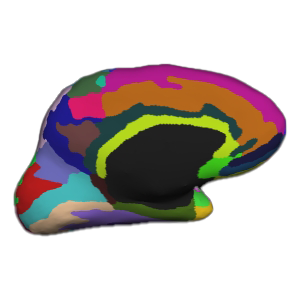
\includegraphics[width=1\linewidth]{3_6_a_destrieux}
    \end{subfigure}%
    \begin{subfigure}[h]{0.5\linewidth}
        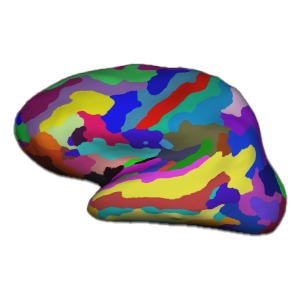
\includegraphics[width=1\linewidth]{3_6_b_destrieux}
    \end{subfigure}
    \caption[Destrieux Atlas]{Destrieux Atlas. Each different color corresponds
    to a specific region of interest.}
\end{figure}
\setchapterstyle{kao}
\chapter{Anatomical Contrastive Learning}
\labch{anatcl}

This chapter will discuss the proposed method that is the subject of this
thesis. To set the stage for the discussion, common approaches in deep learning
applied to neuroimaging and related state-of-the-art works will be reviewed.
Following this, the discussion will shift to an explanation of the various steps
and attempts made to extend existing SOTA approaches, ultimately leading to the
final formulation. Furthermore, the results of the conducted experiments will be
discussed.

\section{Related Works}
Until now, the discussion has primarily focused on the supervised framework of
machine learning. In this framework, as previously explained, the model learns
by using a discriminator (a class label) applied to the data. This approach is
particularly effective when large labeled datasets are available. Deep
convolutional models, for instance, require a substantial amount of data to
learn salient features and regularities within the data, especially pertinent to
brain disorders, which involve clinical, biological, and environmental factors.

However, the availability of large-scale labeled datasets poses a significant
challenge, particularly in the medical field~\sidecite{lan_generative_2020}.
Neuroimaging datasets, for example, typically range from a few hundred to a few
thousand participants, which is considerably smaller compared to the datasets
used for training state-of-the-art classification models\sidenote{For instance,
ImageNet~\cite{deng_imagenet_2009} contains more than 14 million images.}. This
limitation becomes even more pronounced for neuroimaging datasets pertaining to
specific rare disorders.

\subsection{Transfer Learning}
Transfer learning has demonstrated to be a powerful tool to overcome these
limitations in the neuroimaging domain, outperforming standard machine learning
approaches in major tasks related to clinical
psychiatry~\sidecite{dufumier_psychiatry_2024}. Instead of directly learning
from a small labeled dataset in a supervised manner, the transfer learning
paradigm employs a two-phased approach. In the first phase, the model
$f_{\theta}$ is trained on a substantial set of image data of healthy
controls\sidenote{Healthy controls are individuals who do not have the condition
or disease being studied and are used as a standard or baseline for comparison
against those who do have the condition, to identify differences related to the
disease.}. During this phase, the CNN model is trained to learn a
low-dimensional embedding space discovering the general variability associated
with non-specific variables such as, for example, age and sex. The feature
extractor can learn to identify various brain features from the image data
present in the dataset. The result of this process is the set of pre-trained
weights $\theta_{HC}$ of the model on the healthy control data. In the
literature of neuroimaging, the pre-training phase has been implemented in
several ways:
\begin{itemize}
    \item \textbf{Contrastive Learning}: this method involves minimizing the
    distance between encoded representations\sidenote{Encoded representations
    are the output of the encoder.} of same-class pairs while maximizing the
    distance between representations of different-class pairs. Classes are
    determined based on the sample label.
    \item \textbf{Autoregressive Learning}: a Variational AutoEncoder (VAE)
    (\reffig{4_1}) is trained to regenerate the same input image.
    Subsequently, the encoder's weights from the learned VAE are utilized as the
    feature extractor's weights in the pre-trained model.
    \item \textbf{Brain Age Prediction}: when data associated with the age of
    the patient is available, the model is trained to predict the real age
    associated with the patient's brain image data (\reffig{4_2}).
\end{itemize}
\begin{figure*}
    \begin{subfigure}[t]{.45\linewidth}
        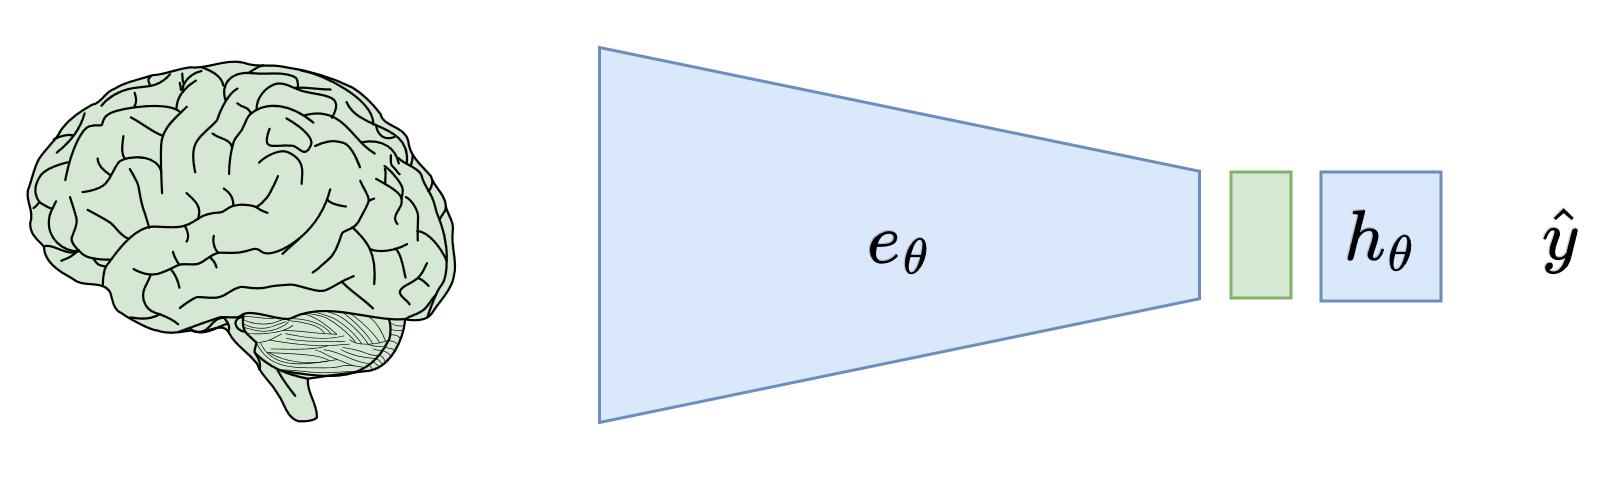
\includegraphics{4_1_age_prediction}
        \caption[Brain Age Prediction Pretraining]{In the brain age prediction
        settings, the encoder $e_\theta$ learns a latent representation of the
        image data that is then used by a discriminator $h_\theta$ to predict
        the age. The predicted age $\hat{y}$ is then confronted with the real
        age $y$ in an appropriate loss function.}
        \labfig{4_1}
    \end{subfigure}
    \hfill
    \begin{subfigure}[t]{.45\linewidth}
        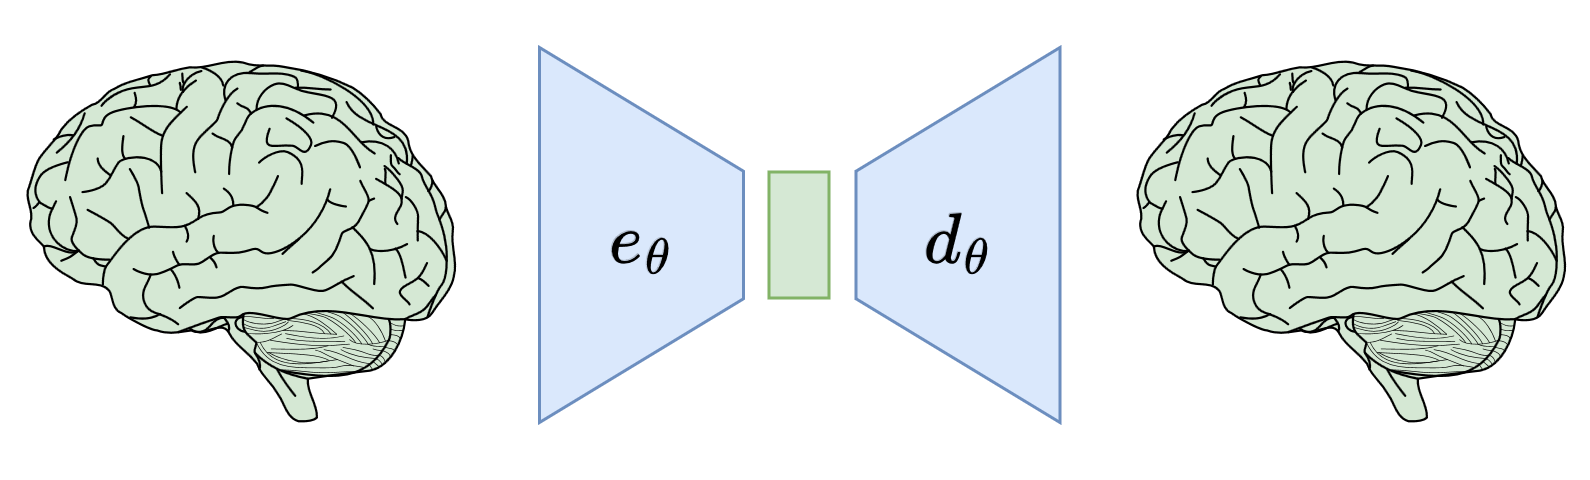
\includegraphics{4_2_vae}
        \caption[Variational Autoencoder Pretraining]{Variational Autoencoders
        consist of an encoder $e_\theta$ that compresses input data into a
        latent space representation (green block) and a decoder $d_\theta$ that
        reconstructs the input data from these encoded representations. In other
        words, the decoder learns to map the latent space back to the original
        data distribution.}
        \labfig{4_2}
    \end{subfigure}
\end{figure*}
After employing the chosen method to pre-train the model, the next phase
involves transferring the trained model on a specific downstream task, using a
dataset of a smaller cohort of patients. Rather than initializing the model
$f_\theta$ with random weights $\theta_{rand}$, it is initialized with the
pre-trained weights $\theta_{HC}$ obtained during the first phase. The
fundamental rationale behind this approach is that by allowing the model to
first learn the general variabilities present in the data, it will requires
significantly less data to subsequently learn the specific features necessary to
distinguish between particular conditions. Although all these pre-training
methods have proven to be extremely effective, a detailed explanation of them is
beyond the scope of this thesis. Given that the current work concentrates on the
contrastive learning framework, it is therefore appropriate to shift the
discussion on this method.

\subsection{Supervised Contrastive Learning}
% TODO: Add another image with augmentation here
\begin{figure}
    \centering
    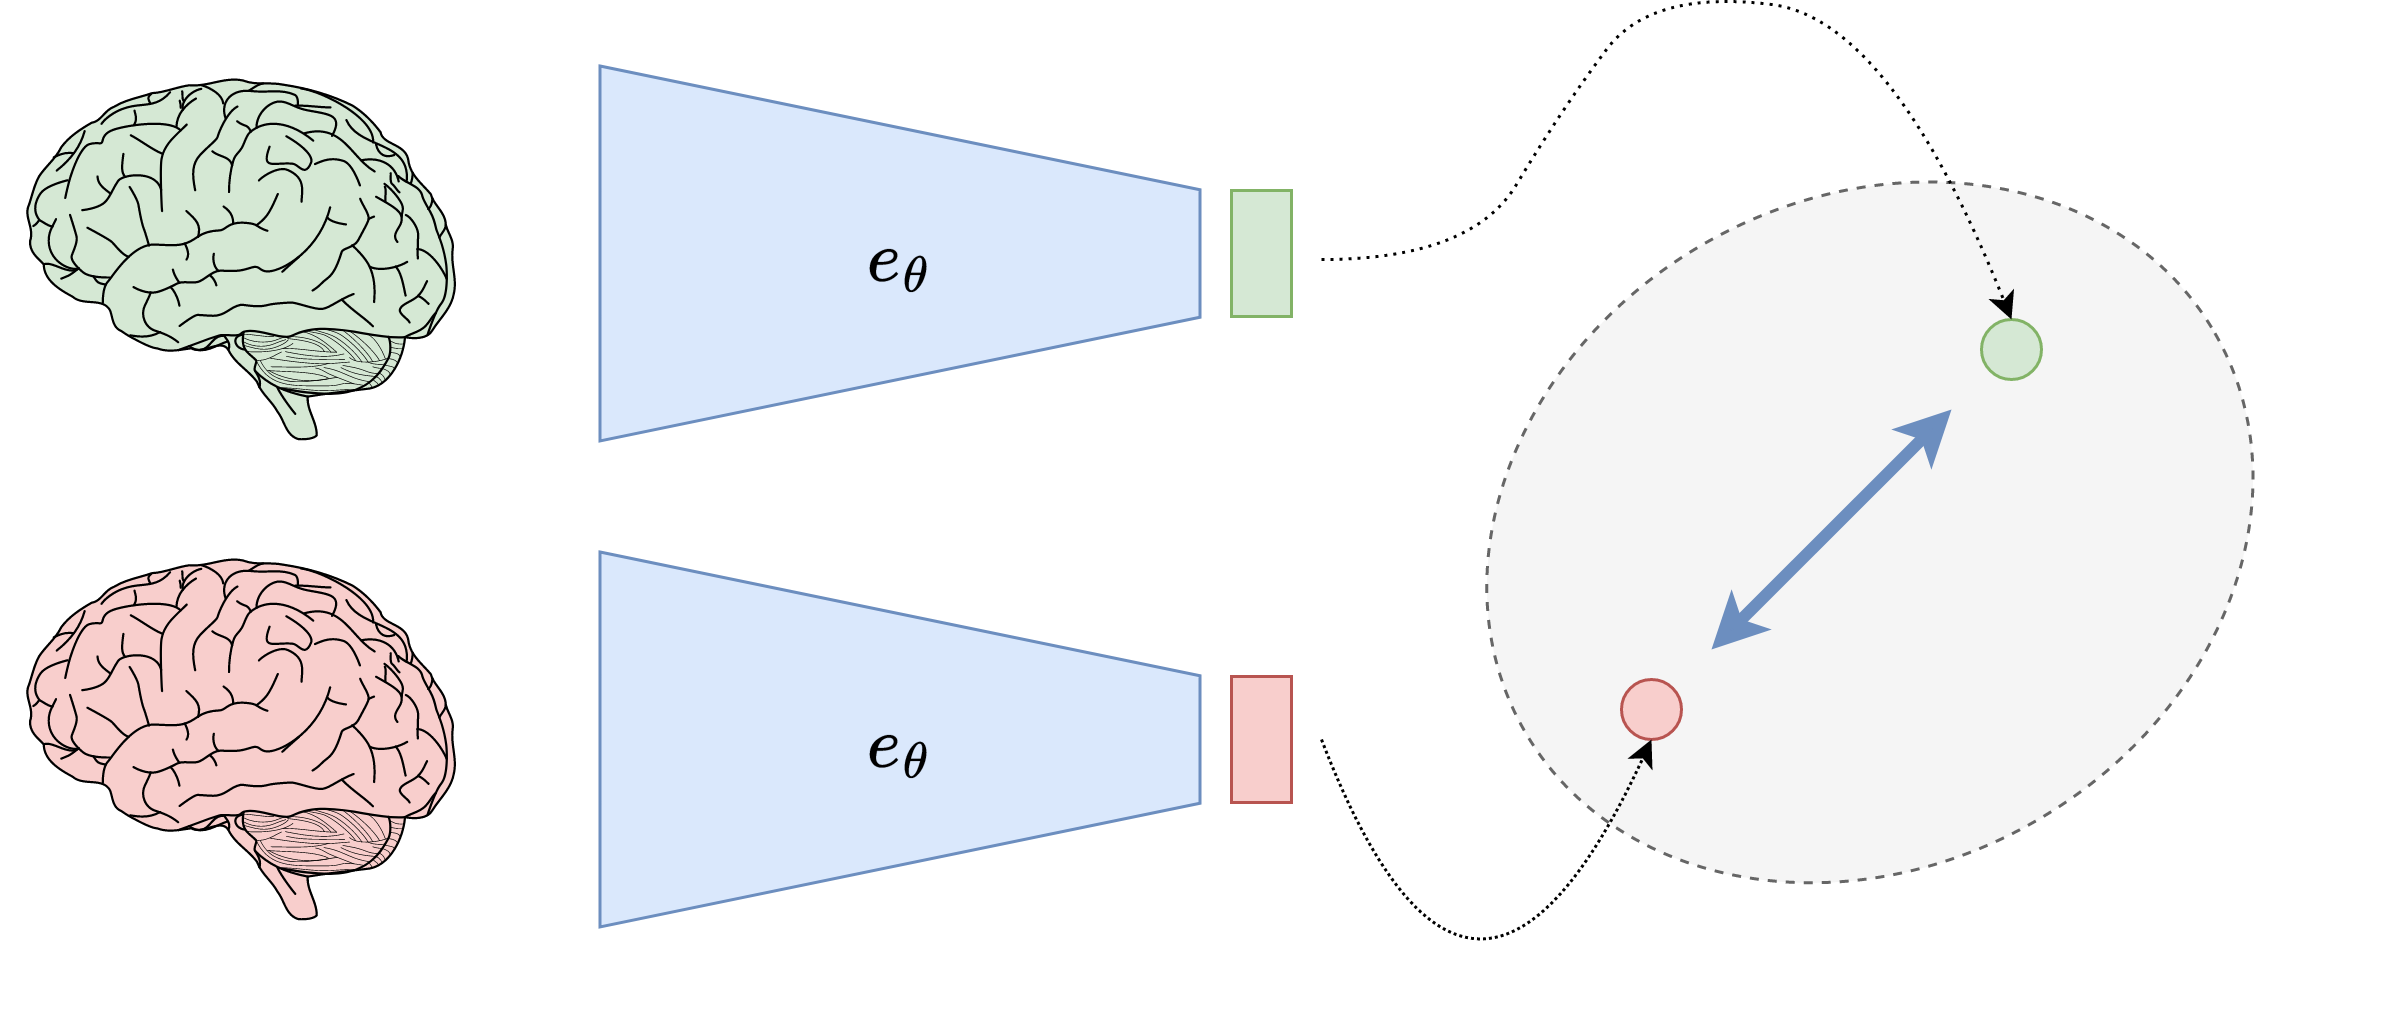
\includegraphics{4_3_contrastive_learning}
    \caption[Contrastive Learning]{The Contrastive Learning method aims at
    maximizing the distance between the latent representations of the anchor
    (green) and the latent representations of negative examples (red).}
    \labfig{4_3}
\end{figure}
As previously mentioned, the foundational principle of the Contrastive
Learning~\cite{hadsell_dimred_2005, chen_self_contrastive_2020,
khosla_supervised_contrastive_2021, henaff_contrastive_2020,
hjelm_contrastive_2019, wu_unsupervised_2018} framework is to develop
representations that draw similar items (positive pairs) nearer in the embedding
space, while distancing dissimilar items (negative pairs). The model
accomplishes this by optimizing a loss function that fosters this specific
behavior. Various loss functions~\cite{schroff_facenet_2015, sohn_improved_2016} have been devised
to foster such behavior, but this discussion will specifically focus on those
used in the supervised context~\sidecite{chen_self_contrastive_2020}. To
establish a more formal foundation for this discussion, consider a neural
network model denoted by $f_\theta$. For any given image and its associated
class label $(x_i, y_i)$ from the dataset, one can compute the latent
representation\sidenote{Also referred to as the \emph{anchor} in this context.}
$z_i = f_\theta(x_i)$. Let also be $I = \{0, \dots, r\}$ the set of indices in
the minibatch, $A(i) = I / i$ the set of indices of all other samples in the
minibatch (except the anchor), and $P(i) = \{p \in A(i) \; : \; y_p = y_i \}$
the set of indices of positive samples\sidenote{Positive in the sense that they
share the same class as the anchor.}.

In the supervised contrastive learning process, each element of the minibatch
$x_i \in \mathcal{B}_r$ is iteratively considered as the anchor. At each step,
each positive sample $x_p$ with $p \in P(i)$ is paired with the anchor to form a
positive pair. Concurrently, the anchor $x_i$ is paired with each remaining
sample $x_a$ with $a \in A(i)$ of the minibatch to form negative pairs. The
objective of the loss is to maximize the similarity\sidenote{Maximizing the
similarity is equivalent to minimizing the distance.} $s_p = sim(z_i, z_p)$
between embeddings of positive pairs, while minimizing the similarity $s_a =
sim(z_i, z_a)$ between negative pairs. The similarity is usually computed though
a \emph{Cosine Similarity}, but can be computed with any similarity measure.
For any anchor $i$, this training objective can be computed using the Supervised
Contrastive (\emph{SupCon}) Loss function, shown in~\refeq{4_1}.
\begin{equation}
    \labeq{4_1}
    \mathscr{L}^{\text{sup}} = 
    - \frac{1}{\lvert P(i) \rvert} \sum_{p \in P(i)} \log \left(
        \frac
        {\exp(s_p / \tau)}
        {\sum\limits_{a \in A(i)} \exp(s_a / \tau)}
    \right)
\end{equation}
Where the term $\tau \in \mathbb{R}^+$ is a scalar value that indicates the
\emph{temperature}\sidenote{The temperature is an hyper-parameter of the loss
function that allows to tune the sensitivity of the loss function to differences
between the distances of positive and negative pairs in the embedding space.} of
the method. The loss of the entire minibatch is simply the sum of the loss
values, considering each element of the minibatch as the anchor.

Models pre-trained with the SupCon loss has shown state of the art accuracy in
classification tasks performed on common labelled imaging
datasets~\cite{chen_self_contrastive_2020}. One of its obvious limitation is
that it needs a large labelled dataset to be applied successfully, which, as
discussed previously, is not the common case of neuroimaging datasets.

\subsection{Self-Supervised Contrastive Learning}
In reality, the SupCon loss is a specific case of a more general function
designed to work in an unsupervised setting. Instead of relying on labels to the
determine the real class of a sample, this method assumes that each sample
belongs to its own unique class. By following this principle, the method applies
an augmentation\sidenote{A series of transformations including cropping,
rotation, and color adjustments, intended to generate a different positive
sample that semantically similar to the original sample but vary in some
features} $Aug(\cdot)$ to the anchor, obtaining another sample $x_j = Aug(x_i)$
that is treated as positive.

The next step is equivalent to the SupCon loss. A positive pair is formed by
means of augmentation to the anchor, and negative pairs are formed using all the
remaining samples in the minibatch. \refeq{4_2} summarizes the Self Supervised
Contrastive loss function.
\begin{equation}
    \labeq{4_2}
    \mathscr{L}^{\text{self}} = - \log \left(
        \frac
        {\exp(s_j / \tau)}
        {\sum\limits_{a \in A(i)} \exp(s_a / \tau)}
    \right)
\end{equation}
Technically speaking, minimizing these loss formulations corresponds to
maximizing the mutual information~\cite{aaron_representation_2018} between
positive pair representations, effectively increasing the amount of shared
information between a positive representation $(z_i)$ and its augmented sample
$(z_j)$. \refeq{4_2} can also be interpreted from a probabilistic perspective.
Through this lens, the numerator can be seen as assigning a high probability to
the event where the anchor and its positive pair are close together in the
embedding space. The denominator acts as a normalization factor, summing the
exponential similarity scores of the anchor with all other embeddings in the
batch (except for itself). This sum transforms the raw exponential scores into
probabilities via the softmax function, thus creating a probability
distribution\sidenote{Also referred to as the \emph{noise} distribution, as it
should include negative samples.} over all pairs involving the anchor and a
negative sample, where pairs with higher similarity scores are assigned higher
probabilities. In essence, the ratio calculates the probability that the anchor
$z_i$ is similar to the positive embedding $z_j$, relative to the probability of
being similar to any other negative embedding $z_a$.

The role of the numerator is to create a "pulling" force between the anchor and
its positive counterpart in the embedding space, ensuring that these connections
are reinforced more strongly during the training process than any other
connections. Conversely, the denominator serves to "push" negative samples away
from the anchor in the embedding space.

However, viewing these loss functions from a probabilistic angle also highlights
a potential issue. These losses assume that all other samples in the minibatch,
aside from the anchor, are negative samples, even though there may be
semantically similar samples to the anchor present in the minibatch. In other
words, other potentially positive samples could be inadvertently included in the
noise distribution.

\subsection{Weakly-Supervised Contrastive Learning}
To address the issue of false negatives in the noise distribution, several
studies have proposed modifications to the aforementioned loss functions. These
adjustments are classified under the umbrella of weakly supervised strategies.
The essence of these strategies is to utilize additional metadata associated
with a sample to define closeness in the embedding space. The underlying
intuition is that samples from similar classes would also share similar
characteristics and, consequently, similar metadata. Augmenting the loss
functions with additional information helps refine the distinction between
positive and negative pairs, improving the effectiveness of the model in
recognizing and differentiating between closely related samples.

In the neuroimaging domain,
\citeauthor{dufumier_contrastive_2021}~\sidecite{dufumier_contrastive_2021}
proposed a method that incorporates the age of a patient associated with a brain
scan as additional metadata. In their research, a contrastive loss function
named \emph{y-aware}\sidenote{This term is used because the model utilizes the
target variable $y$ during the pre-training phase.} was developed. The
fundamental concept of this function is to calculate a weight term $0 \leq w_k
\leq 1$ that determines the \emph{degree of positiveness} of the $k^{th}$ sample
relative to the anchor. To compute this term, the authors suggest applying a
kernel\sidenote{Which could either be a Gaussian or RBF kernel.} $K_\sigma$ to
the age difference between the patients associated with the brain images.
Formally, if $y_k$ is the age attribute associated with the $k^{th}$ sample,
then the weight term is calculated as shown
in~\refeq{4_3}.
\begin{equation}
    \labeq{4_3}
    w_k = K_\sigma(y_i - y_k)
\end{equation}
The role of the kernel $K_\sigma$ in this context is to constrain the difference
value between 0 and 1. The hyper-parameter $\sigma$ determines the spread of the
kernel and can be readily estimated from the dataset.

The weight term $w_k$ is subsequently incorporated into the SupCon loss
formulation by multiplying each pair by its corresponding weight
value\sidenote{Indeed, the original formulation in \refeq{4_1} is a special
case of the \emph{y-aware} function, where weights are implicitly set to either
$1$ or $0$, depending on whether $x_k$ belongs to the same class as $x_i$ or
not.}. This modification allows the model to adjust the influence of each sample
pair in the loss calculation based on their relative age difference.
\refeq{4_4} shows the formulation of the \emph{y-aware loss}.
\begin{equation}
    \labeq{4_4}
    \mathscr{L}^{\text{y-aware}} = 
    -\sum_{k \in A(i)} \frac{w_k}{\sum_t w_t} log
    \left(
    \frac
    {\exp(s_k / \tau)}
    {\sum\limits_{a \in A(i)} \exp(s_a / \tau)}
    \right)
\end{equation}
Pre-trained models that employ the \emph{y-aware} loss have subsequently
achieved state-of-the-art performance in downstream tasks involving the
prediction of neurological pathologies such as Schizophrenia (SCZ), Bipolar
Disorder (BD), and Alzheimer's Disease (AD).

Subsequent research has further explored refinements of the \emph{y-aware} loss
concept. Specifically,
~\citeauthor{barbano_contrastive_2023}~\sidecite{barbano_contrastive_2023}
proposes two extensions to the original formulation. The first refinement arises
from the observation that the uniformity term (the denominator) in \refeq{4_4}
tends to focus more on the closest samples within the representation space. This
concentration means that if positive samples exist elsewhere in the minibatch,
they are inadvertently included in the noise distribution, thus receiving
disproportionately high weighting compared to other negative samples. To address
this issue, the uniformity term is adjusted to include only those samples that
are more distant from the anchor than the considered $x_k$ in the kernel
space. This refinement helps ensure that the term focuses on truly negative
samples, thereby reducing the influence of inadvertently included positive
samples in the noise distribution. \refeq{4_5} shows the proposed loss
function that encodes this behaviour.
\begin{equation}
    \labeq{4_5}
    \mathscr{L}^{\text{thr}} = 
    -\sum_{k \in A(i)} \frac{w_k}{\sum_t \delta_{w_t < w_k} w_t} \log
    \left(
    \frac
    {\exp(s_k / \tau)}
    {\sum\limits_{a \in A(i)} \delta_{w_t < w_k} \exp(s_a / \tau)}
    \right)
\end{equation}
Where $\delta_{c}$ is a step function whose value are $1$ when the condition
$c$ is true or $0$ otherwise.

The other loss function proposed takes an opposite approach. Rather than
repelling the closest "least positive" sample, it adjusts the repulsion strength
(i.e., the weight) on the noise distribution in proportion to their distance
from the anchor in the kernel space. This method ensures that samples farther
away from the anchor exert a greater influence on the noise distribution,
thereby refining how the model discriminates between truly negative and
potentially positive samples within the embedding.
\begin{equation}
    \labeq{4_6}
    \mathscr{L}^{\text{exp}} = 
    -\sum_{k \in A(i)} \frac{w_k}{\sum_t w_t} \log
    \left(
    \frac
    {\exp(s_k / \tau)}
    {\sum\limits_{a \in A(i)} \exp((1 - w_t) s_a / \tau)}
    \right)
\end{equation}
In~\refeq{4_6}, which encapsulates this concept, the weighting factor $(1 -
w_t)$ serves as a negative weighting factor, assigning more weight to samples
that are farther from the anchor in the kernel space. This adjustment emphasizes
the influence of distant samples in the kernel space, effectively pushing them
away from the anchor in the embedding space.

To evaluate these loss functions, a 3D CNN was trained specifically to minimize
the loss function under consideration. After the training of the CNN, a linear
classifier was then trained on the latent representations produced by the CNN,
using a smaller validation dataset. Essentially, the CNN model functions to map
brain images into a more compact representation space, from which a linear
classifier is subsequently trained. In the experiments conducted, the downstream
task for which the linear classifier was trained is brain-age prediction. This
approach allows to assess the effectiveness of the latent space learned by the
CNN and to determine how well the extracted features contribute to estimating
brain age. The experiments conducted demonstrated that the loss function
$\mathcal{L}^{exp}$ yielded superior results, suggesting that
$\mathcal{L}^{exp}$ effectively facilitates the extraction and encoding of
relevant features, that improves the model's predictive capabilities on the
brain-age prediction task.

All of these weakly supervised loss functions have shown promising experimental
results; however, a notable limitation of this class of approaches is their
reliance on a single attribute, such as age, to determine the alignment strength
($w_k$). Consequently, they are not well-suited to leveraging multiple
attributes, such as anatomical measurements of the brain. The method proposed in
the subsequent section addresses this limitation by extending the weakly
contrastive formulation to include multiple attributes, thereby enhancing the
model’s capacity to capture and utilize a broader spectrum of relevant
information.

\section{AnatCL}
To extend the discussed loss functions to include multiple attributes, one of
the initial approaches undertaken involved directly modifying the weight
computation. A straightforward and quick method to consider is to define the
weight as the average of the kernelized differences between each selected
attribute. More formally, if the target attribute $y$ is not just a single
scalar but a vector $\mathbf{y}$ consisting of $L$ attributes, the resulting
weight $w_k$ could be calculated using~\refeq{4_7}.
\begin{equation}
    \labeq{4_7}
    w_k = \frac{1}{L} \sum_{l=0}^{L} K_l ( \mathbf{y}_{i,l} - \mathbf{y}_{k, l} )
\end{equation}
This formulation applies the kernel $K_l$ to the difference between each
attribute $l$ to derive an attribute-wise similarity value. Subsequently, the
mean of these similarity values is calculated to produce a single scalar value.
The mean operation is done to ensures that each attribute contributes equally to
the overall weight, allowing for a balanced integration of multiple
characteristics. Also, in order to accommodate the unique variabilities
associated with each attribute, a different kernel $K_l$ is applied to each
difference.
This initial formulation was first tested using a set of selected
attributes—namely age, CerebroSpinal Fluid Volume (CSFV), Gray Matter Volume
(GMV), and White Matter Volume (WMV)—made available by the OpenBHB
dataset~\sidecite{dufumier_openbhb_2022}. To evaluate the effectiveness of this
new formulation, a 3D ResNet-18 model was pre-trained using this contrastive
loss formulation on the OpenBHB dataset. Subsequently, the model was tested on
the brain-age prediction task using a test split of the dataset. Although this
first approach incorporates more information into the learning process, it
demonstrated a decline in performance compared to counterparts that utilize only
the single age attribute\sidenote{More precisely, in the downstream task of
brain age prediction, the mean squared error (MSE) recorded was 7.29, in
contrast to a significantly lower MSE of 2.66 achieved with the baseline
method.}. The hypothesis is that these anatomical attributes are global features
of the brain that may act as confounders for the
model~\sidecite{komeyer_framework_2024}.

The suboptimal performances observed with this formulation highlighted the need
for a different approach to address this problem. Attention shifted specifically
to another set of anatomical features derived from
the~\citeauthor{desikan_automated_2006} brain
parcellation~\sidecite{desikan_automated_2006}. As previously discussed
in~\refch{neuroimaging}, the Desikan brain parcellation is represented
by a matrix $\mathcal{D} \in \mathbb{R}^{68 \times 7}$, where each row contains
a vector of $7$ features. Each vector represents a set of anatomical features
measured in a specific brain area. Despite offering a richer and more nuanced
representation of anatomical features, the Desikan parcellation presents
challenges due to the multi-dimensional nature of its data. This complexity
poses difficulties in formulating an effective similarity measure, as the
previously discussed loss formulations have primarily addressed scalar feature
values. To incorporate these measurements effectively, it is essential to define
a robust similarity measure between two Desikan parcellations.

\subsection{Local Descriptor}
Two different formulations were hypothesized based on the interpretation of the
Desikan parcellation. The first arises from viewing the Desikan parcellation as
comprised of $68$ vectors of $7$ anatomical measurements. According to this
interpretation, the proposed method to compare two parcellations involves
calculating the pairwise similarity between each corresponding measurement,
resulting in a vector of $68$ similarity values. Each value in this vector
indicates the degree of closeness between the corresponding brain regions in
terms of the recorded anatomical features. Finally, the expected similarity
value across all measurements is then used as the degree of positiveness that
can be subsequently used in one of the weakly contrastive loss formulations
discussed earlier. Since with this interpretation the degree of positiveness is
obtained by computing the expected value of the cross-region similarities, it
has been called \emph{"local descriptor"}.
\begin{figure*}[t]
    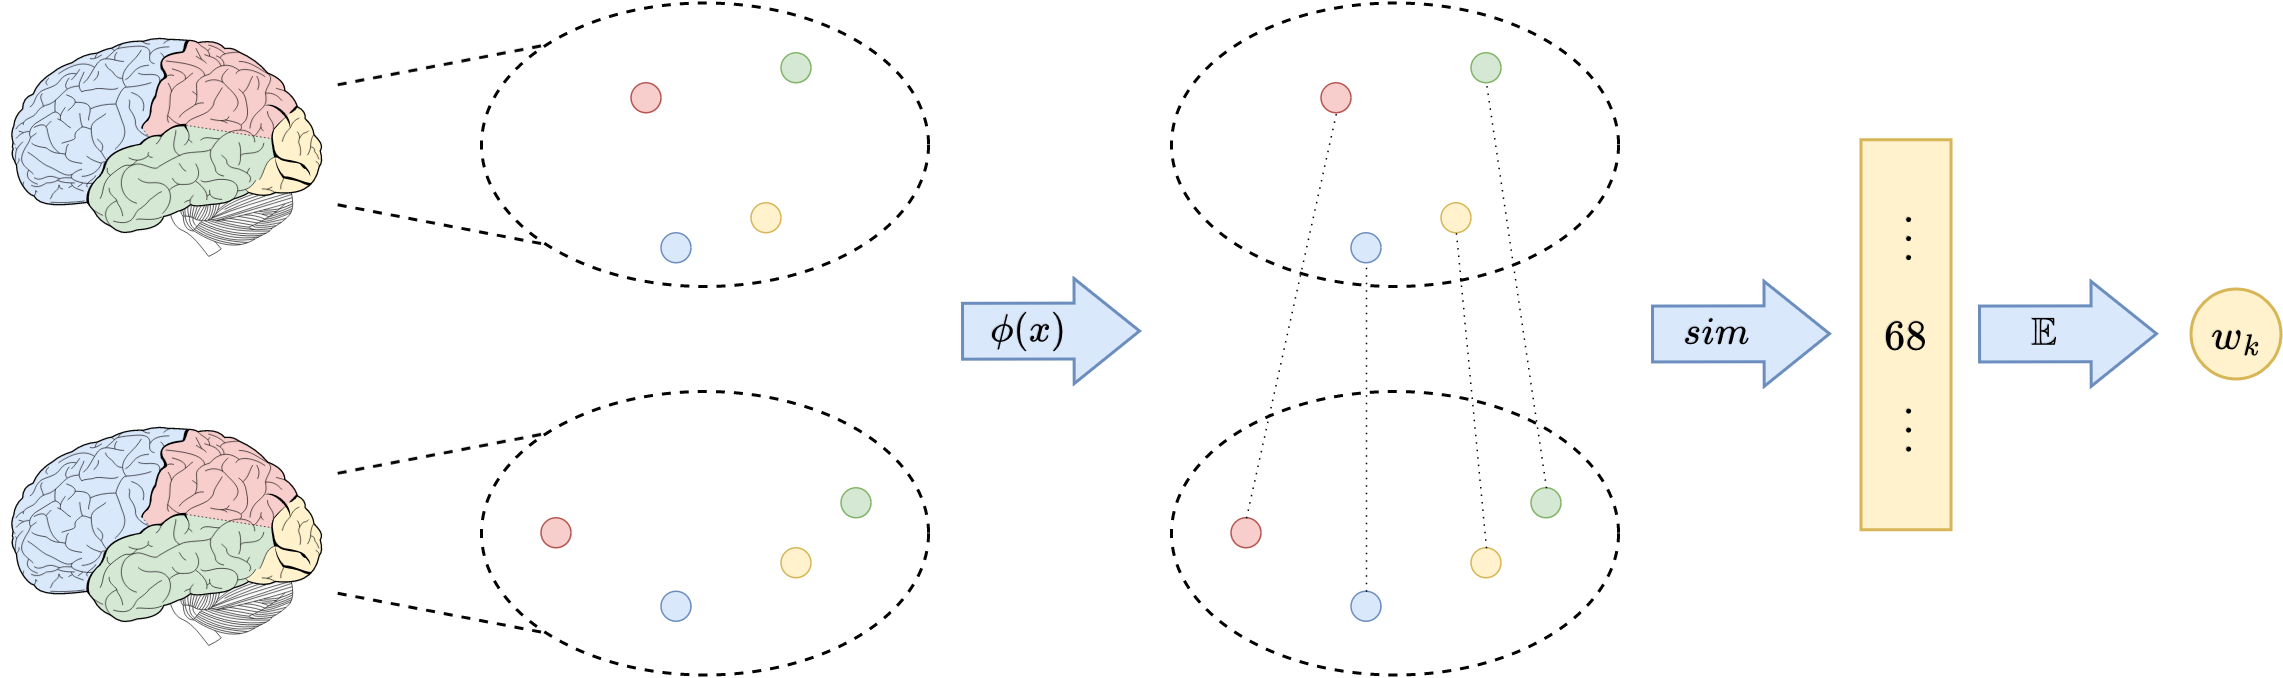
\includegraphics{4_4_local_descriptor}
    \caption[Local Descriptor]{Graphical depiction of the steps required to compute the local
    descriptor. In this interpretation, two different Desikan parcellations are
    visualized as a series of 68 points within a 7-dimensional space. The first
    step in computing the local descriptor involves normalizing these vectors
    through the function $\gamma(x)$, ensuring that they are positioned on the
    unit hypersphere. Following normalization,
    the next step involves calculating the pairwise similarities between each
    measurement vector, resulting in a vector of 68 similarity values. Each
    value reflects the closeness between corresponding brain regions in terms of
    their anatomical features. To determine the final degree of positiveness,
    which quantifies the overall similarity between the two parcellations, the
    expected value $\mathbb{E}$ is computed across the similarity vector.
    }
    \labfig{4_4}
\end{figure*}
Formally, the Desikan parcellation of a $i^{th}$ sample is represented as
$\mathcal{D}^i \in \mathbb{R}^{68 \times 7}$. Each row $\mathcal{D}^i_n$ denotes
the measurement vector for the $n^{th}$ brain region of the $i^{th}$ patient.
Before proceeding with cross-similarity calculations, an adjustment must be made
due to the fact that each feature within a measurement vector captures specific
anatomical information and is recorded on a scale that differs from other
measurements within the vector. To address this variability, a
normalization\sidenote{A transformation used to re-scale values to a range of
$[0;1]$. An example of a normalization is the min-max normalization.}
$\gamma(x)$ is applied to each vector to standardize all measurements.
Following this approach, \refeq{4_8} illustrates the formulation of the
discussed local descriptor.
\begin{equation}
    \labeq{4_8}
    w_k = \frac{1}{68}\sum_{n=1}^{68} sim(\gamma(\mathcal{D}^i_n), \gamma(\mathcal{D}^k_n))
\end{equation}
Where $sim(x, y)$ can be any similarity function\sidenote{In this work the
Cosine Similarity has been mainly used.}. In this case, the $w_k$ term
calculates the atlas-wise similarity of the $k^{th}$ parcellation in relation to
the anchor parcellation $i$.

\subsection{Global Descriptor}
The global descriptor derives from interpreting the Desikan format from another
point of view. Rather than viewing the data as 68 measurement vectors, each
containing 7 different features, this approach considers the format as 7 feature
vectors, each composed of 68 measurement values. Each vector encompasses the
values of a specific measurement recorded across all 68 brain areas. This
reorganization shifts the focus from the regional to the feature-specific
analysis, facilitating a global evaluation that highlights how each individual
anatomical characteristic varies across different brain regions. In other words,
this interpretation arises from considering the transposed version of the
Desikan parcellation, denoted as $\mathcal{D}^T$, which transforms the matrix
into a $7 \times 68$ dimensional format. This transposition shifts the focus from
regional measurements to a feature-centric analysis, allowing each row of the
matrix to represent all the measurements of a specific feature across the 68
brain regions.
\begin{figure}[t]
    \caption[Global Descriptor]{In the corresponding visualization, each brain,
    colored distinctively, represents a specific feature vector, which can be
    depicted in a 68-dimensional space. The global descriptor involves computing
    the cross-similarity, resulting in a 7-element vector that contains
    feature-wise similarities. Similar to the local descriptor, the expected
    value of this vector is calculated to determine the degree of positiveness.}
    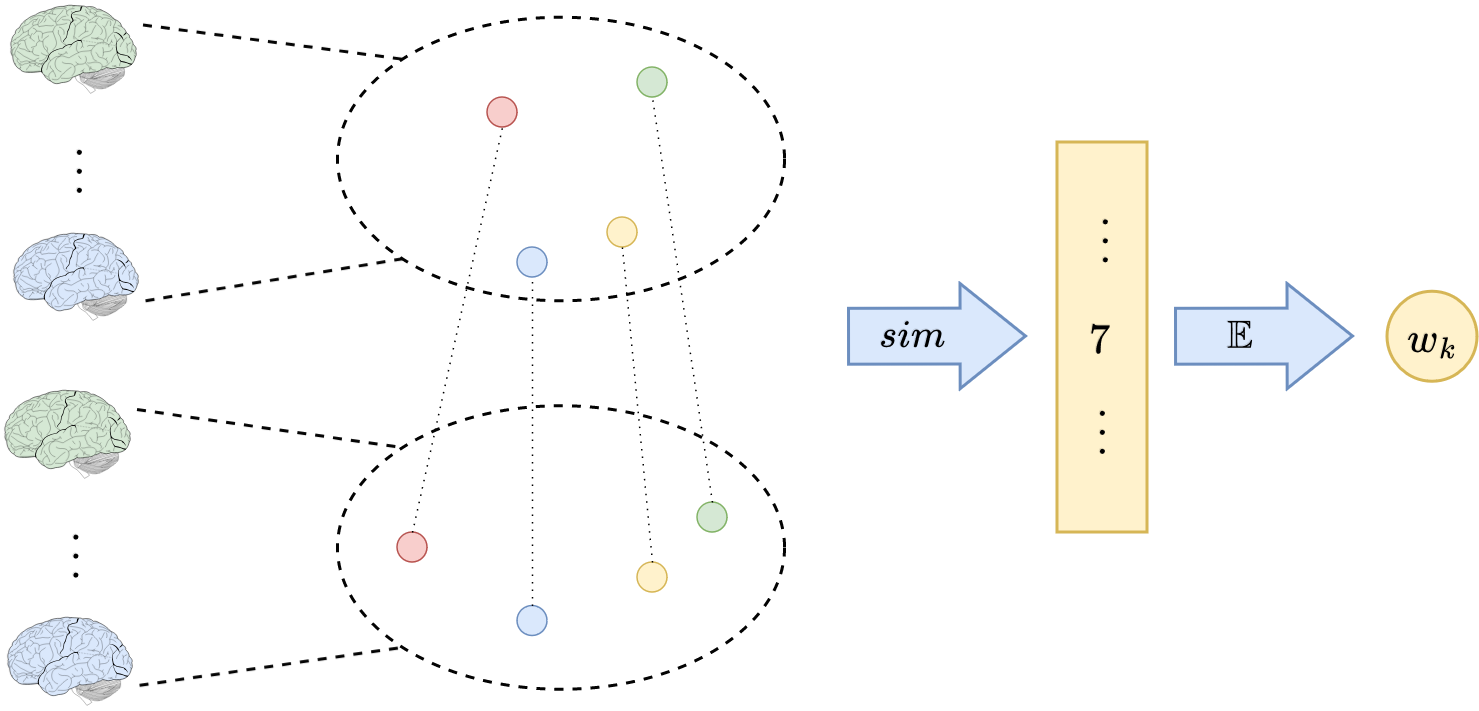
\includegraphics{4_5_global_descriptor}
    \labfig{4_5}
\end{figure}
Since each row of the transposed $\mathcal{D}^T$ matrix contains measurements of
a specific feature across different regions, all data are maintained on a
consistent scale. This uniformity across each vector means that no normalization
step is required before computing the similarity values, simplifying the process
and ensuring that the original measurement scales are preserved during analysis.
\refeq{4_9} shows the formulation of the global descriptor, where $\omega^i_n
= \left( \mathcal{D}^i \right)^T_n$ is the row vector of the transposed
parcellation of the $i^{th}$ sample, containing the 68 measurements pertaining
the $n^{th}$ feature.
\begin{equation}
    \labeq{4_9}
    w_k = \frac{1}{7}\sum_{n=1}^{7} sim(\omega^i_n, \omega^k_n)
\end{equation}
Both the local and global descriptor can then be utilized to calculate the $w_k$
term in one of the weakly supervised contrastive loss formulations previously
discussed. Given that this loss relies on anatomical measures, it has been
designated as $\mathcal{L}^{\text{AnatCL}}$.

To incorporate also the age attribute into the final objective loss, the
resulting function is structured as a weighted sum. This sum combines a weakly
supervised loss that is augmented with the age attribute
($\mathcal{L}^{\text{age}}$) and another weakly supervised loss that utilizes
the anatomical information ($\mathcal{L}^{\text{AnatCL}}$). The specific
formulation of this final objective loss is detailed in \refeq{4_10}.
\begin{equation}
    \labeq{4_10}
    \mathcal{L} = \lambda_1 \mathcal{L}^{\text{age}} + \lambda_2 \mathcal{L}^{\text{AnatCL}}
\end{equation}
In the formulation of the final objective loss function,
$\mathcal{L}^{\text{age}}$ represents any of the previously discussed weakly
supervised loss functions where the computation of the degree of positiveness is
determined using the age attribute. Conversely, $\mathcal{L}^{\text{AnatCL}}$
refers to a weakly supervised loss where the degree of positiveness is computed
using either the local or global descriptor, depending on the specific
anatomical features considered.
Additionally, $\lambda_1, \lambda_2 \in \mathbb{R}$ serve as scalar
hyper-parameters within the loss function. These parameters are used to weigh
the importance of each loss component, thereby determining the preference
between \(\mathcal{L}^{\text{age}}\) and \(\mathcal{L}^{\text{AnatCL}}\).
Adjusting these values allows for fine-tuning of the model's sensitivity to
either the chronological age or the anatomical features, optimizing the balance
based on specific predictive goals or dataset characteristics. 
\begin{figure}
    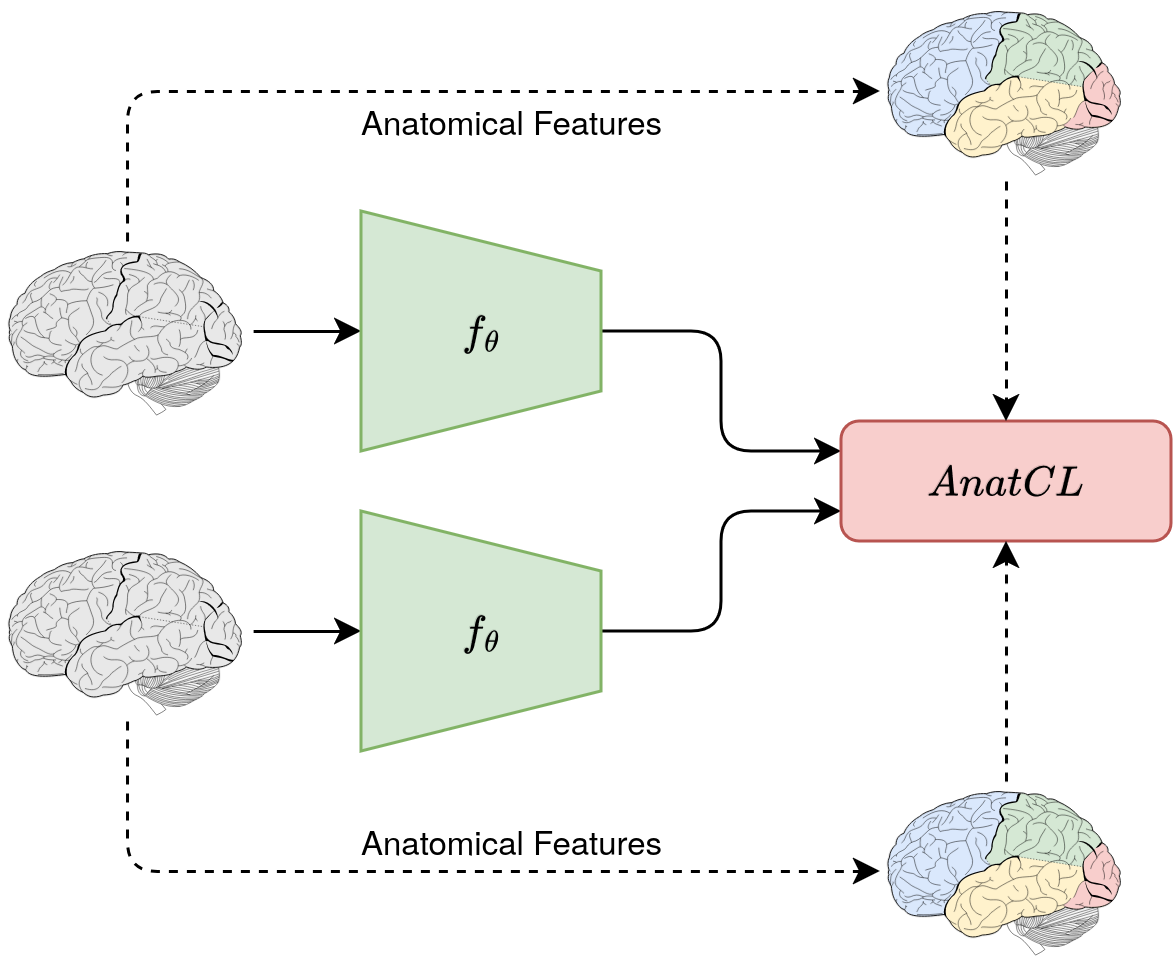
\includegraphics[width=.7\linewidth]{4_6_anatcl_framework}
    \caption[AnatCL Loss Overview]{AnatCL loss overview.}
    \labfig{4_6}
\end{figure}
\setchapterstyle{kao}
\chapter{Experiments}
\labch{experiments}
This chapter outlines the experiments conducted to assess the efficacy of the
proposed loss formulation. To facilitate a comprehensive evaluation, multiple
neuroimaging datasets were utilized, which are described in a dedicated section.
Subsequent to dataset descriptions, the experimental setup is thoroughly
detailed, including the model used and all pertinent training parameters.
Finally, the chapter concludes with several sections, each dedicated to
discussing the experimental results for a specific task that was tested.

\section{Datasets}
Overall, the experimental data consisted of T1-weighted MRI scans, totaling
21,155 images from 7,908 individuals. This data was sourced from various
publicly available datasets, encompassing five different neurological
conditions. The conditions and respective datasets include healthy samples from
OpenBHB~\cite{dufumier_openbhb_2022}, Alzheimer's Disease from
ADNI~\cite{petersen_alzheimer_2010} and OASIS-3~\cite{lamontagne_oasis_2019},
schizophrenia from SchizConnect~\cite{wang_schizconnect_2016}, and Autism
Spectrum Disorder from ABIDE I~\cite{ABIDE}. This diverse compilation of
datasets provided a robust foundation for evaluating the proposed loss
formulation and its effectiveness across different neurological conditions.
The overall composition of the cohorts used in this study is presented in~\reftab{5_1}.
\begin{table}[h]
    \centering
    \caption[Cohorts Composition]{An overview of the various datasets utilized
    in this study, along with their cohort compositions.}
    \begin{tabular}{l l c}
    \toprule
    \textbf{Condition} & \textbf{Dataset} & \textbf{Patients}  \\
    \midrule
    Healthy Control & OpenBHB & 3984 \\
    Schizophrenia & SchizConnect & 383 \\
    Alzheimer's Disease & ADNI & 1754 \\
    Alzheimer's Disease & OASIS-3 & 685 \\
    Autism Spectrum Disorder & ABIDE-I & 1102 \\
    \bottomrule
    \end{tabular}
    \labtab{5_1}
\end{table}

\subsection{OpenBHB} OpenBHB is a newly released dataset that consolidates
healthy control (HC) samples from numerous public cohorts including ABIDE 1,
ABIDE 2, CoRR, GSP, IXI, Localizer, MPI-Leipzig, NAR, NPC, and RBP. Each scan in
this dataset originates from a different subject, making it uniquely suited for
ensuring diversity in the training process. In addition to structural scans and
patient information\sidenote{Some of them are age, sex, total intracranial
volume, acquisition settings.}, OpenBHB provides seven anatomical measures based
on the Desikan-Killiany parcellation~\cite{desikan_automated_2006}. As
previously discussed, such measures include cortical thickness (mean and
standard deviation), gray matter volume, surface area, integrated mean, Gaussian
curvature index, and intrinsic curvature index~\cite{dufumier_openbhb_2022}. 

\subsection{ADNI}
The Alzheimer's Disease Neuroimaging Initiative (ADNI) is a significant research
project that was launched to study Alzheimer's disease through the collection
and analysis of medical imaging, genetic, biological markers, and clinical
assessment data. ADNI is aimed at understanding the progression of Alzheimer's
Disease from its earliest stages, through mild cognitive impairment (MCI), to
full Alzheimer's Dementia (AD). Over the years, several phases of the
Alzheimer's Disease Neuroimaging Initiative (ADNI) have been undertaken, each
contributing to the growing body of data on Alzheimer's Disease and its
precursors. The specific phases include ADNI-1, ADNI-2, ADNI-GO, and ADNI-3. For
the experiments conducted, data from all these different ADNI phases were
utilized, comprising a diverse cohort of participants. This included 633 healthy
controls (HC), 712 patients diagnosed with mild cognitive impairment (MCI), and
409 patients diagnosed with Alzheimer's Disease (AD).

\subsection{OASIS-3}
The Open Access Series of Imaging Studies (OASIS-3) is a neuroimaging dataset
specifically designed for studying the progression of Alzheimer’s disease across
different stages. OASIS-3 builds upon earlier versions of the dataset (OASIS-1
and OASIS-2) by incorporating a larger and more diverse set of data points,
which includes both longitudinal and cross-sectional data. The dataset contains
a demographic of participants ranging from young adults to older adults with
varying stages of cognitive decline, including normal aging individuals, those
with Mild Cognitive Impairment (MCI), and those diagnosed with Alzheimer’s
disease. For the experiments conducted with this dataset, 685 patients were
included, containing 88 AD cases.

\subsection{SchizConnect}
SchizConnect is a dataset that emerged from a collaborative research effort
aimed at consolidating neuroimaging data from multiple studies and sites. It
includes participants diagnosed with schizophrenia, schizoaffective disorder,
other related psychotic disorders, and healthy control individuals. From the
SchizConnect database, anatomical MRIs were included for the experiments, for a
total of 383 patients. This cohort is categorized as follows: 180 are healthy
controls (HC), 102 are classified under schizophrenia (broad), 74 under
schizophrenia (strict), 11 as schizoaffective patients, and 9 with bipolar
disorder.

\subsection{ABIDE I}
The Autism Brain Imaging Data Exchange I (ABIDE-I) is an open-source initiative
designed to support research into Autism Spectrum Disorder (ASD). ABIDE-I
encompasses a comprehensive dataset comprising resting-state functional magnetic
resonance imaging (rs-fMRI) scans, anatomical scans, and phenotypic information
from over 1,000 individuals, ranging in age from 6 to 64 years. This diverse
group includes both individuals diagnosed with ASD and age-matched control
subjects without ASD, providing a robust resource for comparative studies.

In the conducted experiments, anatomical MRIs from ABIDE-I were utilized,
involving a total of 1,102 participants. This cohort was categorized into 556
healthy controls (HC), 339 patients diagnosed with autism, 93 patients with
Asperger's Syndrome, and 7 diagnosed with pervasive developmental disorder not
otherwise specified (PDD-NOS). 

\section{Experimental Settings}
\begin{figure*}
    \begin{subfigure}[t]{.45\linewidth}
        \caption{Pre-train phase}
        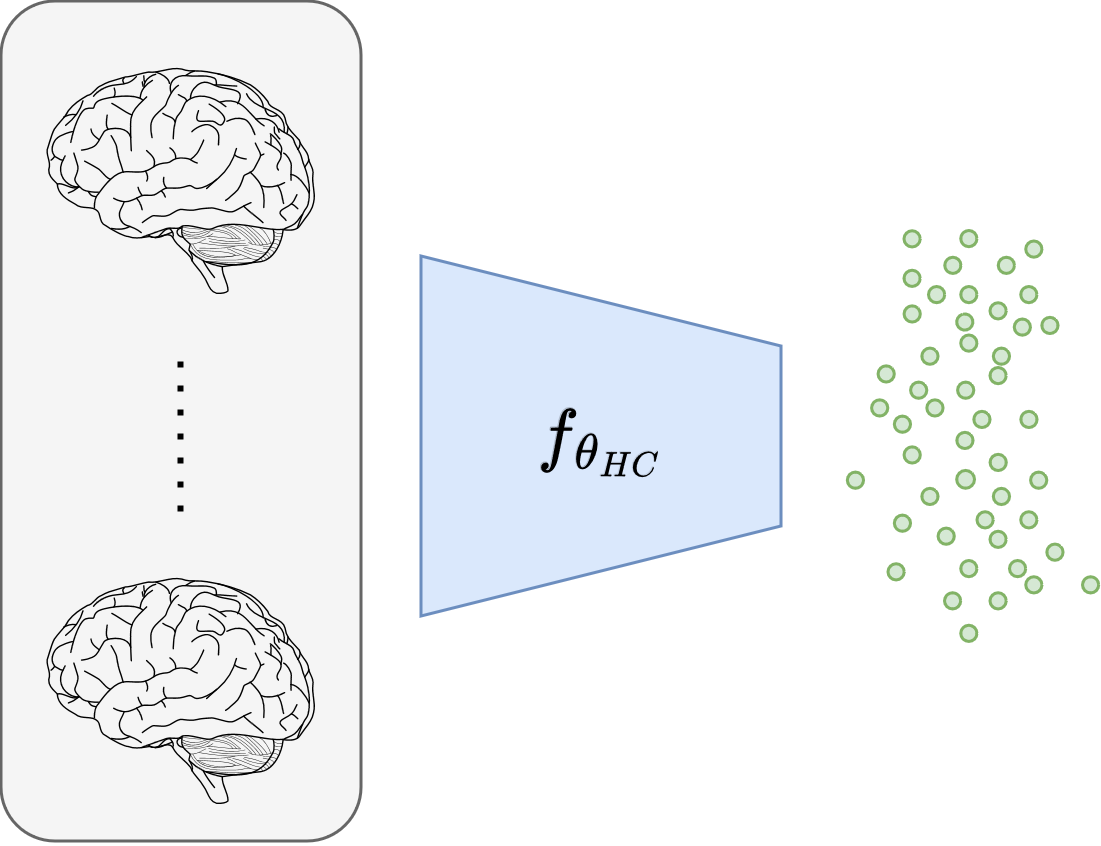
\includegraphics{5_1_a_pretrain}
    \end{subfigure}
    \hfill
    \begin{subfigure}[t]{.45\linewidth}
        \caption{Downstream transfer phase}
        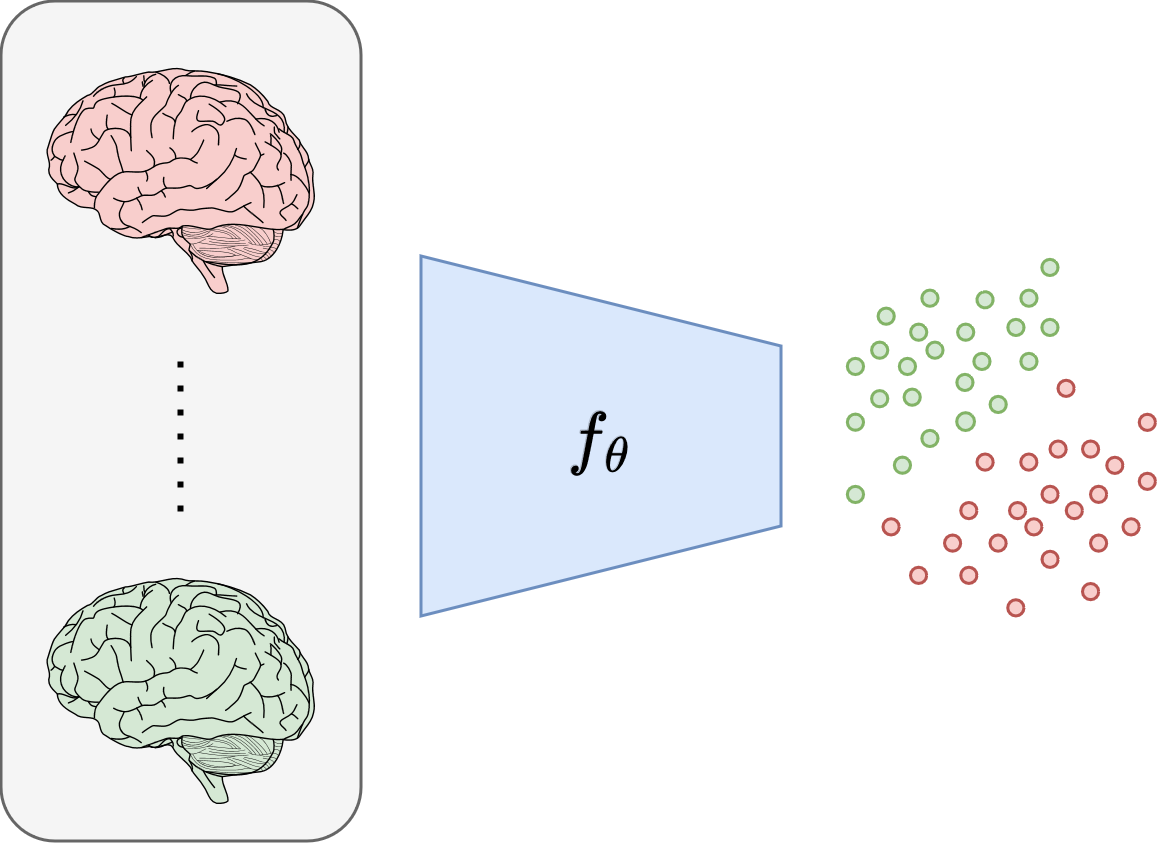
\includegraphics{5_1_b_transfer}
    \end{subfigure}
    \caption[Experimental Settings (Transfer Learning)]{
    The experimental settings adhere to the principles of transfer
    learning. Initially, a model $f$ (depicted in blue) is pre-trained on a
    substantial cohort of healthy subjects (represented by the grey box),
    utilizing the OpenBHB dataset in this instance. The outcome of this initial
    phase is a model $f_{\theta_{HC}}$, which has captured general variabilities
    within the data; that is, it has learned the latent \emph{manifold}. In the
    subsequent phase, the model is adapted to a downstream task. This involves
    mapping the images into the learned latent space, after which a conventional
    machine learning model is employed to perform the classification.
    }
    \labfig{}
\end{figure*}
Before initiating any experiments, to ensure uniformity across all images, they
underwent a standardized VBM preprocessing protocol using
CAT12~\cite{gaser_cat_2022}. This preprocessing included non-linear registration
to the MNI template and extraction of gray matter (GM). The images were brought
to a final spatial resolution of 1.5mm isotropic and sized to 121 x 145 x 121.
The preprocessing tasks were carried out using the BrainPrep
package~\sidecite{grigis_brainprep_2022}. The experiments specifically utilized
modulated gray matter (GM) images, as indicated by
~\citeauthor{dufumier_openbhb_2022}~\cite{dufumier_openbhb_2022}, to ensure that
the volumetric information was retained in the images for detailed analysis.

The experiments followed a two-phased approach aligned with the transfer
learning paradigm. Initially, a target model was pre-trained using the proposed
contrastive learning loss on the OpenBHB dataset. Subsequently, the model was
tested on various downstream tasks across different datasets to assess its
performance and generalization capabilities. Practically, in the proposed losses
(\refeqshort{4_7}, \refeqshort{4_8}), only a subset of the anatomical
measurements available in the Desikan format were utilized\sidenote{Specifically
Cortical Thickness (CT), Gray Matter Volume (GMV), and Surface Area (SA).}.
These losses are henceforth referred to as AnatCL-G3 for the global descriptor
version using three measurements and AnatCL-L3 for the corresponding local
descriptor.

The experimental settings for both loss formulations, local (AnatCL-L3) and
global (AnatCL-G3), were identical. Two ResNet-18 3D models were pre-trained
using VBM-preprocessed images along with their corresponding Desikan measures
based on the proposed formulations. The training process utilized the Adam
optimizer with a learning rate of 0.0001 and a decay rate of 0.9 applied every
10 epochs. The models were trained with a batch size of 32 for a total of 300
epochs. For simplicity, the values of $\lambda_1$ and $\lambda_2$ were both set
to 1. As is standard practice in contrastive learning approaches
~\cite{chen_self_contrastive_2020, khosla_supervised_contrastive_2021}, the
contrastive loss was computed using a fully-connected projection head following
the encoder, which consisted of two layers.

To endure a robust evaluation, the experimental setup included cross-validation,
where each of the 5 folds was structured with a 70\% training split and a 30\%
test split. This distribution ensured that each fold had a substantial amount of
data for training the models, while still providing a significant portion for
testing and evaluating model performance across different iterations. The
results were then quantified in terms of mean and standard deviation across the
5 folds, providing a comprehensive assessment of model performance and stability
across different test scenarios.

After the pre-training step, the models underwent evaluation by testing their
performance using a transfer learning approach. In this approach, latent
representations were first generated by the model using only the encoder
section, discarding the fully connected head\sidenote{This step ensures that the
evaluation focuses on the quality of the features extracted by the encoder,
rather than the classification capabilities of the full network.}. For each
downstream task, a different linear classifier was trained on these extracted
representations to assess the model's ability to learn meaningful and
generalizable features. The rationale behind this methodology was to isolate the
effectiveness of the learned representations from the specific architecture of
the downstream task classifiers. By focusing on the encoder's output, the
evaluation could better determine whether the fundamental features extracted
during pre-training were robust and informative enough to facilitate accurate
classifications across various conditions, independent of the subsequent
classifier configurations.

The downstream tasks primarily focused on predicting specific diagnoses (such as
Alzheimer's Disease, Schizophrenia, Bipolar Disorder, etc.), biomarkers (e.g.,
brain age), or phenotypes (e.g., sex). Additionally, other relevant clinical
assessments included in the datasets were also considered, which will be
explained in detail in~\refsec{cognitive_scores}. A total of 22 downstream tasks
were tested, which are summarized in~\reftab{5_2}.
\begin{table*}[h]
    \centering
    \caption[Downstream Tasks Summary]{Summary of downstream tasks (12) and
    clinical assessment scores (10) considered in the study.}
    \begin{tabular}{l l}
    \toprule
    \textbf{Dataset} & \textbf{Task / Condition} \\
    \midrule
    OpenBHB & Age (HC)   \\
            & Sex   \\
    ADNI    & Alzheimer's Disease \\
            & sMCI vs pMCI \\
    OASIS-3 & Alzheimer's Disease \\
    SchizConnect & Schizophrenia Broad \\
                 & Schizophrenia Strict \\
                 & Bipolar Disorder \\
                 & Schizoaffective \\
    ABIDE I & Autism \\
            & Aspergers \\
            & PDD-NOS \\
    \bottomrule
    \end{tabular}
    \begin{tabular}{l l}
    \toprule
    \textbf{Dataset} & \textbf{Phenotype}  \\
    \midrule
    SchizConnect  & AIMS Overall Severity  \\
                  & AIMS Upper Body \\
                  & AIMS Lower Body \\
                  & Depression \\
                  & Handedness \\
                  & SAS GAIT \\
    ABIDE 1 & Handedness \\
            & FIQ (WASI)\\
            & VIQ (WASI) \\
            & PIQ (WASI) \\
    & \\
    & \\
    \bottomrule
    \end{tabular}
    \labtab{5_2}
\end{table*}
For the comparative analysis with standard approaches, four different baseline
methodologies were also tested alongside the proposed method. These included the
completely self-supervised loss, known as SimCLR \sidenote{This loss was
introduced by the authors of the corresponding
paper~\cite{chen_self_contrastive_2020} and is referenced as such.}
(\refeqshort{4_2}), and three supervised baselines: a standard model trained
with the L1 loss \sidenote{An L1 loss function calculates the mean of the
absolute differences between the labels and the predictions.}, y-Aware
(\refeqshort{4_4}), and ExpW (\refeqshort{4_6}). To ensure consistency and
fairness in the evaluation, all these methods were subjected to the same
experimental setup as previously described. In this way, the comparative results
accurately reflect the relative performance of each method under identical
conditions.
All the experiments were implemented in PyTorch~\cite{paszke_2017} and run on a
cluster of 4 NVIDIA V100 GPUs\sidenote{The computational resources were provided
by the Leonardo supercomputer, which is managed by the CINECA consortium.}, with
each training session taking approximately 10 hours. 

\section{Diagnosis Prediction}
\begin{figure}
    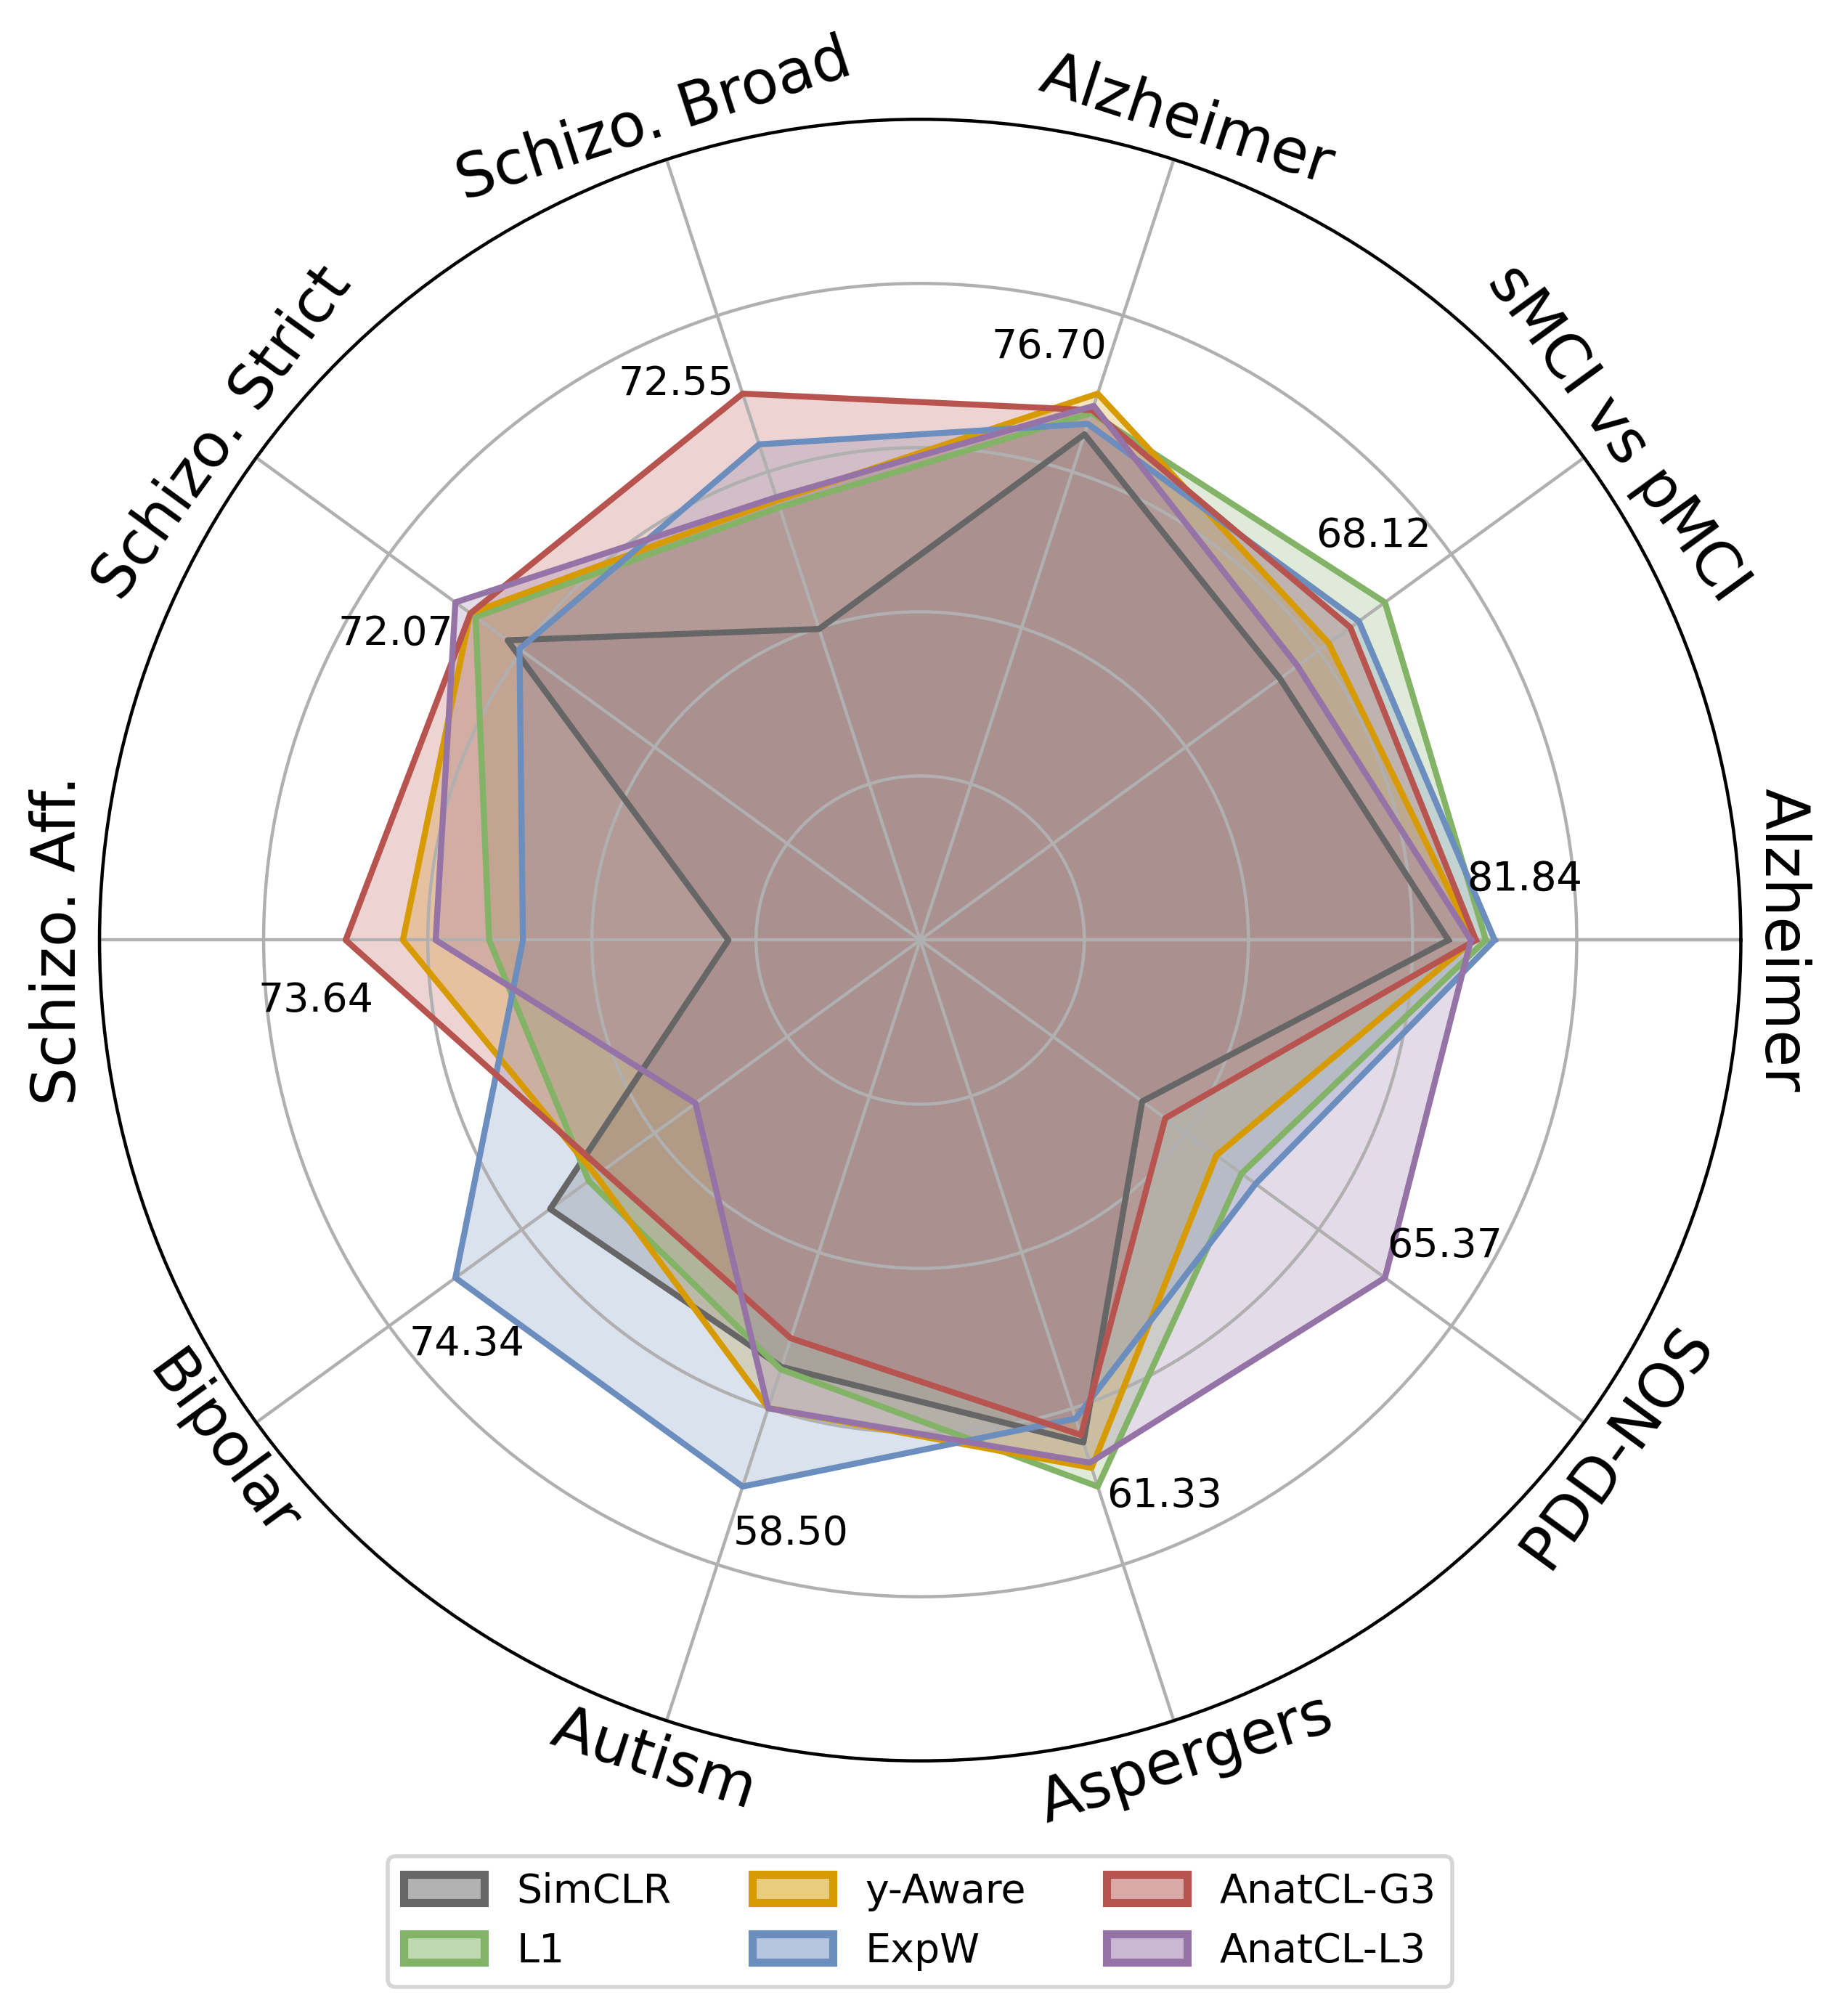
\includegraphics{5_2_polar_plot}
    \caption[Polar Plot of Various Tested Losses]{A polar plot that summarize
    the performances of the various loss functions discussed in this chapter.}
    \labfig{5_2}
\end{figure}

\subsection{Brain Age and Sex Prediction}
Preliminary results focusing on brain age prediction and sex classification were
evaluated using the OpenBHB dataset. These results are detailed
in~\reftab{5_3}. Analysis of the findings indicates that the
AnatCL model is capable of matching and slightly exceeding state-of-the-art
performance in brain age prediction tasks. It is important to note that no
bias-correction methods were employed in this study, despite recommendations
suggested by~\citeauthor{mayoral_biological_2023}~\cite{mayoral_biological_2023}
and ~\citeauthor{delange_commentary_2020}~\cite{delange_commentary_2020}. In
terms of sex classification, while the AnatCL model does not outperform the ExpW
approach, it does show improvements over the SimCLR and L1 loss baselines.
\begin{table}[!h]
    \centering
    \caption[Brain-Age Prediction Results]{Results on OpenBHB in terms of mean
    absolute error (MAE) on age prediction, and balanced accuracy on sex
    classification.}
    \begin{tabular}{l c c}
    \toprule
    \textbf{Method} & \textbf{Age MAE} & \textbf{Sex}  \\
    \midrule
    SimCLR & \result{5.58}{0.53} & \result{76.7}{1.67} \\
    %
    L1 (age sup.) & \result{2.73}{0.14} & \result{76.7}{0.67} \\
    %
    y-Aware & \result{2.66}{0.06} & \result{79.6}{1.13} \\
    %
    ExpW & \result{2.70}{0.06} & \textbf{\result{80.3}{1.7}} \\
    \midrule
    %
    AnatCL-G3 & \textbf{\result{2.61}{0.08}} & \result{78.2}{1.25} \\
    AnatCL-L3 & \result{2.64}{0.07} & \result{78.2}{0.7}\\
    \bottomrule
    \end{tabular}
    \labtab{5_3}
\end{table}

\subsection{Alzheimer's disease and Cognitive Impariments}
In~\reftab{5_4}, the results for Alzheimer's Disease (AD) detection using the
ADNI and OASIS-3 datasets are presented. Although the AnatCL model does not
achieve the best results overall, it generally shows improvements over the
self-supervised baseline (SimCLR) and occasionally surpasses the performance of
either the L1, y-Aware, or ExpW models. This indicates that while AnatCL may not
yet be the top-performing model across all metrics, it demonstrates potential by
consistently outperforming a self-supervised approach and, in some cases, other
supervised methodologies. This suggests that further refinement and adaptation
of the AnatCL approach could lead to more competitive results in AD detection
tasks, as will be discussed in \refch{conclusions_future_developments}.
\begin{table}[!h]
    \centering
    \caption[Alzheimer's Disease Results]{Results on Alzheimer's Disease (AD)
    classification in terms of balanced accuracy.}
    \begin{tabular}{l c c | c}
    \toprule
    & \multicolumn{2}{c|}{\textbf{ADNI}} & \multicolumn{1}{c}{\textbf{OASIS-3}}\\
    \textbf{Method} & \textbf{HC vs AD} & \textbf{sMCI vs pMCI} & \textbf{HC vs AD} \\
    \midrule
    SimCLR & \result{78.47}{2.51} & \result{61.77}{3.85} & \result{73.97}{4.98} \\
    L1 (age sup.) & \result{81.20}{2.3} & \textbf{\result{68.12}{5.42}} & \result{75.40}{5.4} \\
    y-Aware & \result{80.3}{1.8} & \result{64.72}{4.43} & \textbf{\result{76.70}{3.30}} \\
    ExpW & \textbf{\result{81.84}{2.95}} & \result{66.54}{5.64} & \result{74.67}{2.87} \\
    \midrule
    AnatCL-G3 & \result{80.47}{2.95} & \result{66.03}{2.93} & \result{75.59}{2.67}\\
    AnatCL-L3 & \result{80.11}{1.0} & \result{62.83}{4.5} & \result{75.88}{3.0}\\ 
    \bottomrule
    \end{tabular}
    %}
    \labtab{5_4}
\end{table}


\subsection{Schizophrenia and Bipolar Disorders}
The performance of downstream tasks on SchizConnect was evaluated for detecting
schizophrenia (broad and strict), schizoaffective, and bipolar disorders. The
results, detailed in~\reftab{5_5}, show that with the AnatCL model,
state-of-the-art performance was achieved in three out of the four tasks. This
underscores the value of incorporating anatomical information into the model,
particularly for these psychiatric conditions.

\begin{table*}[h]
    \caption[Schizophrenia Detection Results]{Results on schizophrenia detection
    (SCZ) in terms of balanced accuracy.}
    \begin{tabular}{l c c c c}
    \toprule
    &\multicolumn{4}{c}{\textbf{SchizConnect}}\\
    \textbf{Method} & \textbf{SCZ. (Broad)} & \textbf{SCZ (Strict)} & \textbf{Schizoaff.} & \textbf{Bipolar}\\
    \midrule
    SimCLR & \result{58.53}{3.52} & \result{68.47}{8.47} & \result{51.23}{11.94} & \result{67.34}{9.96}\\ 
    %
    L1 & \result{65.79}{4.74} & \result{70.68}{5.10} & \result{65.24}{15.21} & \result{64.49}{22.08} \\
    %
    y-Aware & \result{66.20}{4.50} & \result{71.04}{2.31} & \result{70.29}{14.73} & \result{63.95}{19.81} \\
    %
    ExpW & \result{69.53}{4.43} & \result{67.65}{8.27} & \result{63.26}{18.06} & \textbf{\result{74.34}{18.95}} \\
    %
    \midrule
    AnatCL-G3 & \textbf{\result{72.55}{5.16}} & \result{71.03}{8.53} & \textbf{\result{73.65}{7.29}} & \result{63.43}{15.94}\\
    %
    AnatCL-L3 & \result{66.38}{5.96} & \textbf{\result{72.07}{8.42}} & \result{68.37}{8.60} & \result{56.60}{11.48}\\
    \bottomrule
    \end{tabular}
    \hfill
    \labtab{5_5}
\end{table*}

\subsection{Autism Spectrum Disorder}
Additionally, the performance in detecting Autism Spectrum Disorder (ASD) across
three categories—autism, Asperger's, and PDD-NOS—is also reported
in~\reftab{5_6}. While AnatCL did not outperform other methods for autism and
Asperger's patients, it significantly improved accuracy for diagnosing patients
with PDD-NOS, a relatively rarer diagnosis within the dataset.
\begin{table}[h]
    \centering
    \caption[Autism Spectrum Disorder Detection Results]{Results on autism
    spectrum disorder (ASD) detection in terms of balanced accuracy.}
    \begin{tabular}{l c c c}
        \toprule
        &\multicolumn{3}{c}{\textbf{ABIDE-I}}\\
        \textbf{Method} & \textbf{Autism} & \textbf{Aspergers} & \textbf{PDD-NOS}\\
        \midrule
         SimCLR & \result{54.45}{2.99} & \result{59.61}{2.72} & \result{52.12}{6.62} \\
         L1 & \result{54.53}{1.79} & \textbf{\result{61.33}{8.77}} & \result{57.54}{5.93} \\
         y-Aware & \result{55.84}{3.37} & \result{60.60}{9.22} & \result{56.17}{10.17} \\
         ExpW & \textbf{\result{58.50}{2.41}} & \result{58.68}{3.82} & \result{58.31}{4.33} \\
         \midrule
         AnatCL-G3 & \result{53.48}{0.99} & \result{59.32}{6.58} & \result{53.38}{5.86} \\
         AnatCL-L3 & \result{55.85}{1.02} & \result{60.40}{2.29} & \textbf{\result{65.37}{6.73}} \\
         \bottomrule
    \end{tabular}
    \labtab{5_6}
\end{table}

Overall, AnatCL consistently outperformed or matched the other baselines,
demonstrating its efficacy across a diverse range of psychiatric conditions.
This suggests that AnatCL's approach to integrating detailed anatomical features
significantly contributes to its ability to detect nuanced differences in
neuroimaging data associated with various psychiatric diagnoses.

\section{Cognitive Scores/Assessments Prediction}
\labsec{cognitive_scores}
In the final experiments, the focus shifts to predicting clinical assessment
scores from brain MRIs, a topic that, to the best of current knowledge, has not
been extensively explored in other studies. Specifically, for the SchizConnect
dataset, evaluations included the Abnormal Involuntary Movement Scale (AIMS)
assessed across three domains (overall, upper body, lower body), a Depression
score based on the Calgary Scale, Handedness information, and GAIT measurements
with the Simpson-Angus-Scale (SAS). For the ABIDE dataset, assessments also
included handedness and three IQ scores\sidenote{IQ scores were measured using
the Wechsler Abbreviated Scale (WASI)}: Full Scale IQ (FIQ), Visual IQ (VIQ),
and Performance IQ (PIQ). 
\begin{figure*}[t]
    \begin{subfigure}[t]{.45\linewidth}
        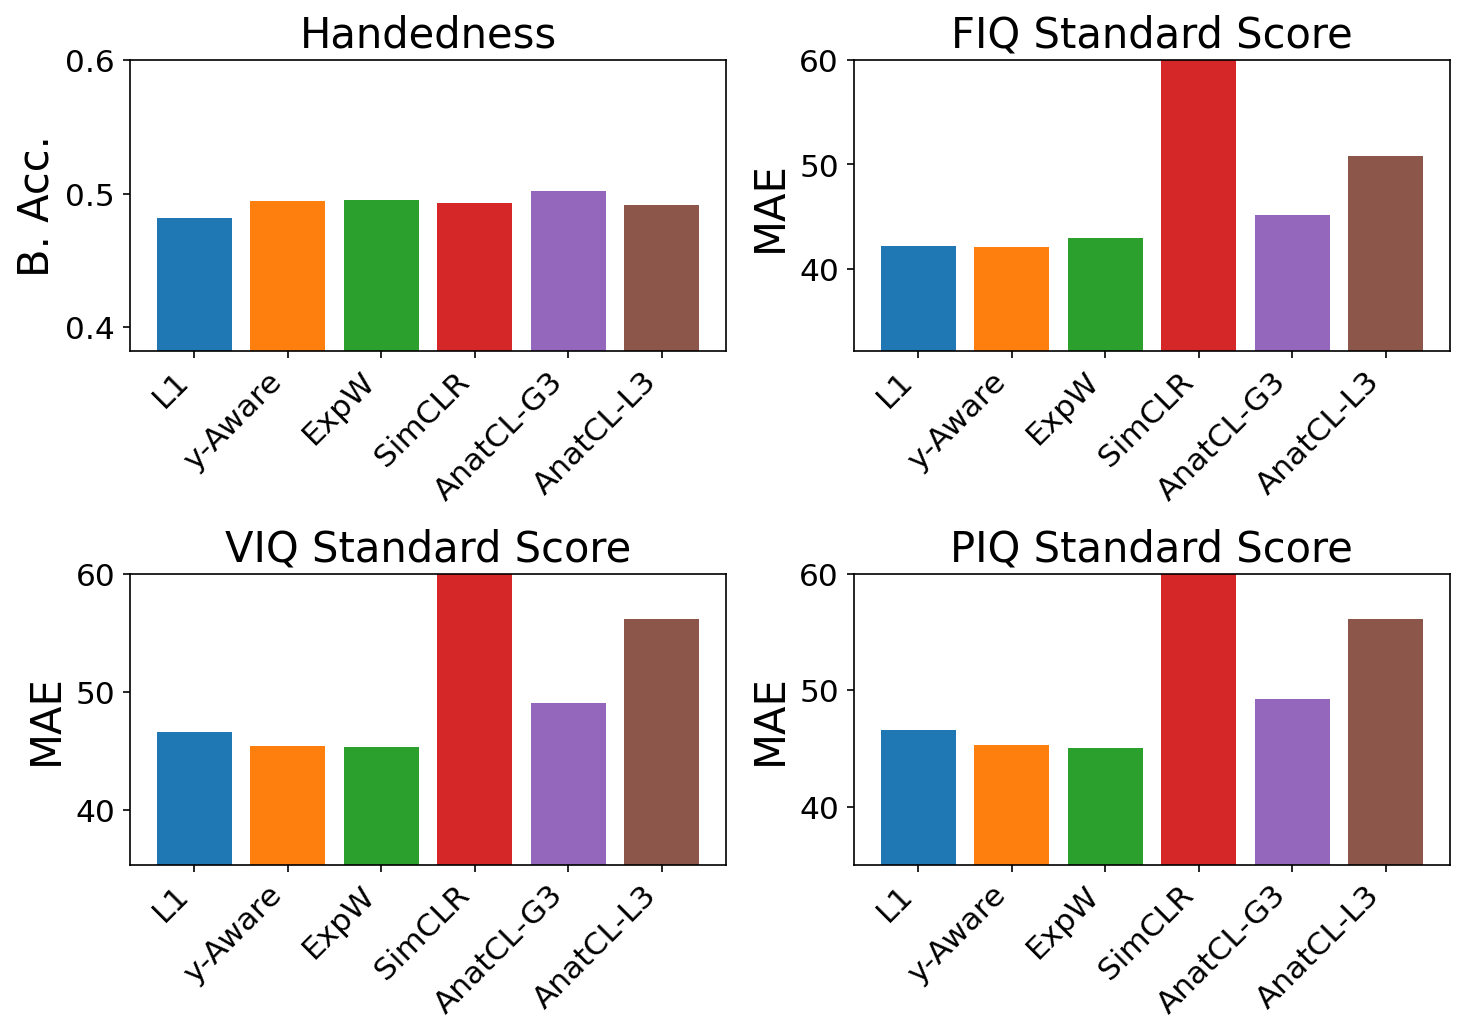
\includegraphics{5_3_a_abide_barplot}
        \caption{}
        \labfig{5_3_a}
    \end{subfigure}
    \hfill
    \begin{subfigure}[t]{.45\linewidth}
        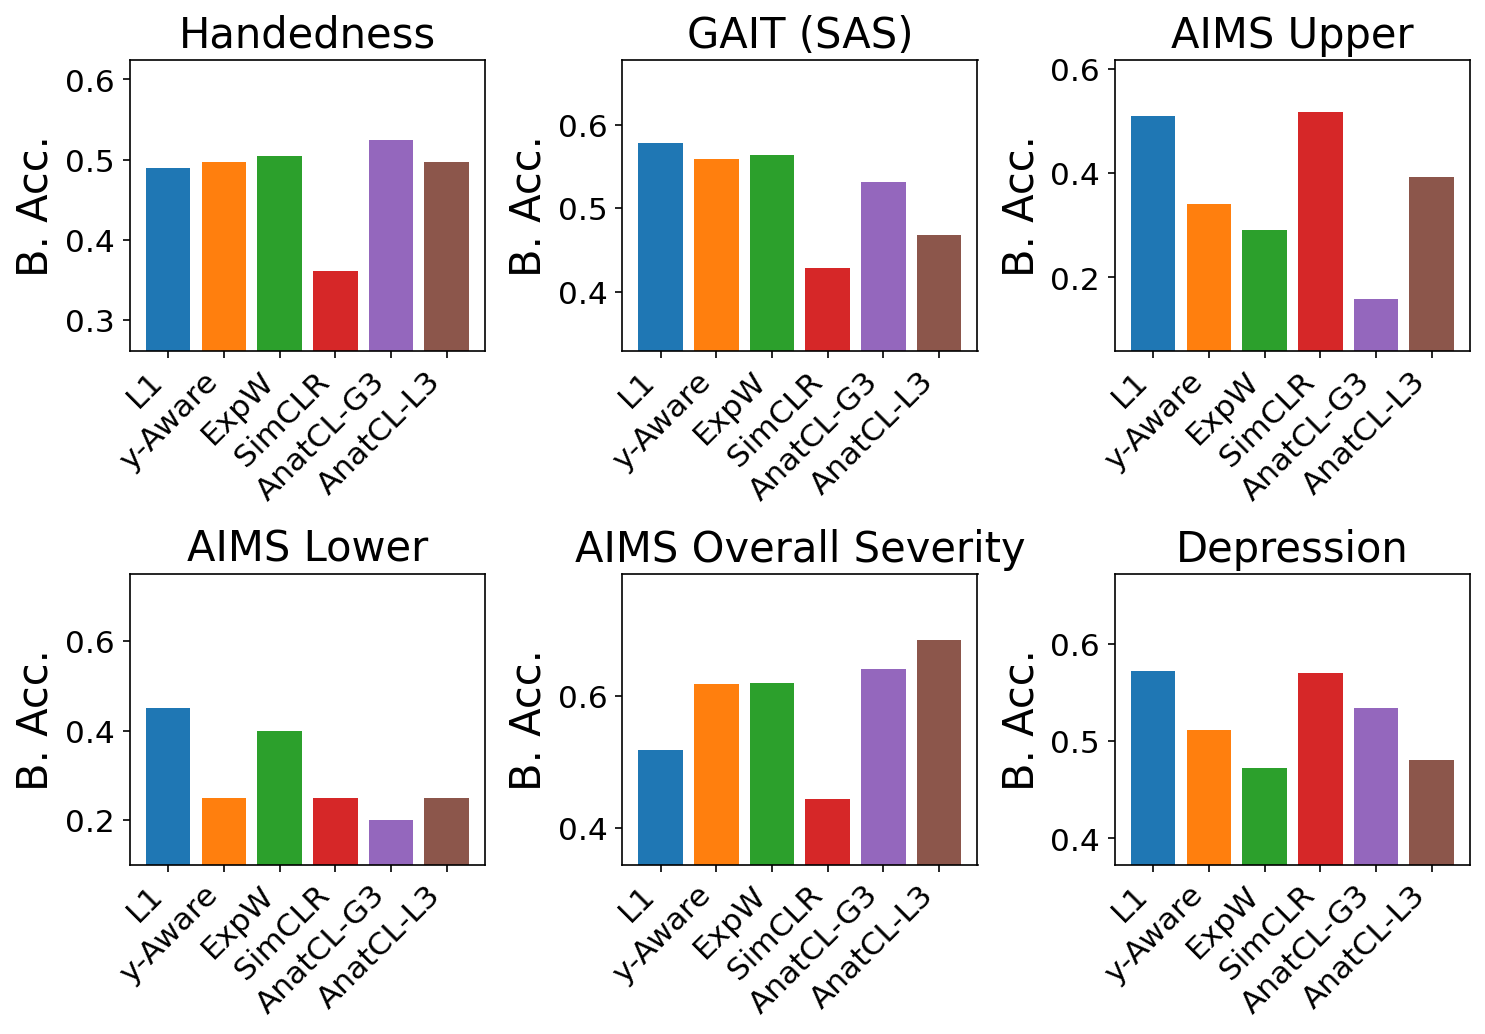
\includegraphics{5_3_b_schiz_barplot}
        \caption{}
        \labfig{5_3_b}
    \end{subfigure}
    \caption[Results Summary (Bar Plots)]{Bar plot format summarization of the
    results discussed. Subfigure~\ref{fig:5_3_a} refers to the ABIDE-I dataset,
    while subfigure~\ref{fig:5_3_b} on the SchizConnect.}
\end{figure*}

\begin{table*}[!b]
    \centering
    \caption[Assessment Scores Results on SchizConnect]{Results of assessment scores/phenotypes prediction from brain MRIs on the SchizConnect dataset.}
    \resizebox{\linewidth}{!}{%
    \begin{tabular}{l c c c c c c}
    \toprule
    & \multicolumn{6}{c}{\textbf{SchizConnect}}\\
     \textbf{Method} & \textbf{AIMS Overall} & \textbf{AIMS Up.} & \textbf{AIMS Low.} & \textbf{Depression} & \textbf{Handedness} & \textbf{GAIT} \\
    \midrule
    SimCLR & \result{44.33}{29.92} & \textbf{\result{51.67}{16.16}} & \result{25.00}{27.39} & \result{56.93}{13.88} & \result{36.06}{2.72} & \result{42.83}{9.61}\\
    %
    L1 & \result{51.83}{24.43} & \result{50.83}{20.82} & \textbf{\result{45.00}{33.17}} & \textbf{\result{57.17}{13.06}} & \result{48.91}{5.60} & \textbf{\result{57.73}{8.64}} \\
    %
    y-Aware & \result{61.83}{15.87} & \result{34.17}{11.90} & \result{25.00}{27.39} & \result{51.09}{5.32} & \result{49.71}{7.69} & \result{55.92}{9.52}\\
    %
    ExpW & \result{62.00}{12.40} & \result{29.17}{17.08} & \result{40.00}{33.91}
    & \result{47.26}{7.27} & \result{50.39}{6.28} &
    \result{56.39}{14.14}\\
    \midrule
    %
    AnatCL-G3 & \result{64.00}{12.72} & \result{15.83}{12.19} & \result{20.00}{18.71} & \result{53.35}{8.54} & \textbf{\result{52.44}{9.14}} & \result{53.10}{11.69} \\
    AnatCL-L3 & \textbf{\result{68.50}{18.09}} & \result{39.17}{14.81} &
    \result{25.00}{27.39} & \result{48.05}{10.89} & \result{49.67}{8.06} &
    \result{46.74}{5.05}\\
    \bottomrule
    \end{tabular}
    }
    \labtab{5_7}
\end{table*}

The ten phenotypes considered are divided based on the nature of the prediction
task: AIMS, depression, handedness, and GAIT are approached as classification
tasks, while IQ scores (FIQ, VIQ, and PIQ) are treated as regression tasks. More
precisely, for handedness, the model predicts right-handed versus other
(left-handed or ambidextrous); for depression, it classifies between absent
versus mild and above; for AIMS, it differentiates between none and minimal
versus mild and above; and for GAIT, it categorizes as normal versus everything
else The results of these experiments on the SchizConnect dataset are reported
in \reftab{5_7}, while the results regarding the ABIDE-I dataset
are reported in \reftab{5_8}.

\begin{table*}[!h]
    \caption[Assessment Scores Results on ABIDE-I]{Results of assessment scores/phenotypes prediction from brain MRIs on the ABIDE-I dataset.}
    \begin{tabular}{l c c c c}
    \toprule
    & \multicolumn{4}{c}{\textbf{ABIDE-I}} \\
    \textbf{Method} & \textbf{Handedness} & \textbf{FIQ (MAE)} & \textbf{VIQ (MAE)} & \textbf{PIQ (MAE)}\\
    \midrule
    SimCLR & \result{49.26}{5.78} & \result{84.65}{16.36} & \result{89.07}{15.14} & \result{89.68}{15.00}\\
    %
    L1 & \result{48.18}{9.43} & \result{42.16}{31.17} & \result{46.54}{32.57} & \result{46.64}{32.24}\\
    %
    y-Aware & \result{49.45}{1.56} & \textbf{\result{42.10}{31.14}} &
    \result{45.38}{33.19} & \result{45.35}{32.76} \\
    %
    ExpW  & \result{49.53}{3.26} & \result{42.94}{30.76} &
    \textbf{\result{45.28}{33.23}} & \textbf{\result{45.02}{32.88}} \\ 
    %
    AnatCL-G3 & \textbf{\result{50.21}{6.82}} & \result{45.18}{29.68} & \result{49.07}{31.52} & \result{49.30}{30.86} \\
    %
    AnatCL-L3 & \result{49.13}{3.32} & \result{50.77}{27.14} &
    \result{56.18}{28.06} & \result{56.13}{27.62}\\
    \bottomrule
    \end{tabular}
    \hfill
    \labtab{5_8}
\end{table*}

While it cannot be concluded that any of the analyzed methods can accurately
predict all clinical assessments from MRI scans, AnatCL overall achieves the
best results in three out of ten cases, which surpasses any other baseline
method. Interestingly, AnatCL shows a better capability to predict the overall
AIMS score and patients' handedness. This suggests that there may be a link
between brain anatomy and these specific phenotypes, highlighting the potential
of anatomically informed models in understanding and predicting behavioral
traits.


\setchapterstyle{kao}
\chapter{Conclusions and Future Developments}
\labch{conclusions_future_developments}

In conclusion, the extensive validation across ten different downstream tasks,
as discussed in~\refch{anatcl}, has demonstrated that integrating anatomical
information during training enhances the accuracy of predictions for various
neurological and psychiatric conditions. The findings also indicate a partial
improvement in the accuracy for clinical assessment scores and phenotypes. These
results suggest that enriching these learning methods with anatomical data can
yield more robust and generalizable models applicable to a range of downstream
tasks. The insights gained from these models could be crucial in developing
personalized treatment plans for patients. By accurately characterizing the
neurological basis of various psychiatric and neurodegenerative disorders, these
models could significantly influence the design of tailored therapeutic
interventions. Additionally, achieving higher accuracy in detecting biomarkers
such as brain age from these models could significantly enhance the diagnosis of
specific neurological disorders, thereby improving patient outcomes. 

However, further research is required to refine and enhance these methods. For
example, an obvious limitation of this approach is that these methods still rely
on the age attribute, which may not be available in all neuroimaging datasets.
Further research in this area could lead to the development of novel methods
that rely solely on anatomical measures for weak supervision, potentially
achieving superior performance compared to fully self-supervised methods. Since
anatomical measures can be automatically extracted using established
neuroimaging algorithms, these innovative methods could essentially be
considered fully self-supervised.

Furthermore, this research primarily utilized a specific brain atlas, thereby
not incorporating the range of other atlases available in the neuroimaging
literature. Future work could involve exploring additional atlases that utilize
different anatomical measures. Such an endeavor would necessitate a meticulous
comparative evaluation of these alternative atlases to determine their efficacy
and accuracy relative to the one used in this study. Expanding the scope to
include a variety of atlases could enhance the robustness and applicability of
the findings, potentially offering a more comprehensive understanding of brain
anatomy and its implications for neuroimaging analysis.

Another potential direction not explored in this thesis involves utilizing other
acquisition methods as additional learning data. The aim would be to integrate
diverse neuroimaging modalities (sMRI, fMRI, dMRI), signals (EEG) and other
relevant data (clinical assessment scores, phenotypic data) into the learning
process of the model. The idea is to create a more holistic model that
incorporates a broader range of modalities in order to provide a more
comprehensive understanding of brain health and pathology. The integration of
diverse sources of information could be achieved either by incorporating it into
the loss formulation, as examined in this work, or by developing a novel
multimodal model architecture capable of extracting and combining salient
information from input data.
Recent research~\sidecite{radford_clip_2021} has also demonstrated the
feasibility of augmenting deep learning models not only with imaging data but
also with textual data. For instance, in the medical domain, there has been a
research effort~\sidecite{wang_medclip_2022} directed towards integrating
clinical records and assessment scores. This research direction is further
supported by recent works~\sidecite{venugopalan_multimodal_2021} that
demonstrated by integrating data of different nature such as EEG and clinical
assessments could significantly enrich the representations learned by the model.

The findings from this research direction could pave the way for the development
of large multimodal models that could serve as foundational tools in
personalized medicine. Employing the principles of transfer learning, these
models can be adapted for personalized predictions of psychiatric conditions,
such as Autism Spectrum Disorder (ASD), and neurodegenerative conditions, such
as Alzheimer's Disease (AD). To achieve this, multimodal and/or longitudinal
data can be utilized to create detailed, patient-specific profiles and to model
the progression of various conditions. Such personalized models can then offer
customized insights and treatment recommendations, thereby enhancing patient
outcomes by accommodating the unique variations in brain structure and function
specific to each individual.

\section*{Ethical Considerations}
In the development and experiments described within this thesis, strict
adherence to ethical standards was maintained. A significant aspect of these
ethical considerations involves the use of data. It is important to note that
there were no ethical issues concerning the datasets utilized, as all were
publicly accessible and composed of previously anonymized patient data, ensuring
that individual privacy was preserved and that the data could be used without
compromising patient confidentiality.

Furthermore, the applications of the findings discussed in this research thesis
are aimed at enhancing the accuracy of diagnoses and the identification of
pathological conditions related to the brain. By improving diagnostic
capabilities through more precise imaging analysis, the potential for positive
impacts on patient outcomes is significant. The use of advanced machine learning
models in medical imaging can lead to earlier detection of diseases, more
tailored treatment plans, and ultimately, better patient care. This alignment
with the goal of improving healthcare outcomes further supports the ethical
justification for this research.

\section*{Declaration of Originality}
I declare to be responsible for the content I'm presenting in order to
obtain the final degree, not to have plagiarized in all or part of, the work
produced by others and having cited original sources in consistent way with
current plagiarism regulations and copyright. I am also aware that in case of
false declaration, I could incur in law penalties and my admission to final exam
could be denied.

% Uncomment if you want to add appendix.
% \appendix % From here onwards, chapters are numbered with letters, as is the appendix convention
% \pagelayout{wide} % No margins
% \addpart{Appendix}
% \pagelayout{margin} % Restore margins

% % \setchapterstyle{lines}
% \labch{appendix}
% % Fist Appendix
% \chapter{Fonts Testing}

% \section{Font Sizes}

% {\tiny The quick brown fox jumps over the lazy dog.}

% {\scriptsize The quick brown fox jumps over the lazy dog.}

% {\footnotesize The quick brown fox jumps over the lazy dog.}

% {\small The quick brown fox jumps over the lazy dog.}

% {\normalsize The quick brown fox jumps over the lazy dog.}

% {\large The quick brown fox jumps over the lazy dog.}

% {\Large The quick brown fox jumps over the lazy dog.}

% {\LARGE The quick brown fox jumps over the lazy dog.}

% {\huge The quick brown fox jumps over the lazy dog.}

% {\Huge The quick brown fox jumps over the lazy dog.}


% \section{Font Families}

% \sffamily\blindtext

% \textmd{The quick brown fox jumps over the lazy dog. Medium.}

% \textbf{The quick brown fox jumps over the lazy dog. Bold.}

% \textup{The quick brown fox jumps over the lazy dog. Upright.}

% \textit{The quick brown fox jumps over the lazy dog. Italics.}

% \textsl{The quick brown fox jumps over the lazy dog. Slanted.}

% \textsc{The quick brown fox jumps over the lazy dog. Small Caps.}

% \ttfamily\blindtext

% \textmd{The quick brown fox jumps over the lazy dog. Medium.}

% \textbf{The quick brown fox jumps over the lazy dog. Bold.}

% \textup{The quick brown fox jumps over the lazy dog. Upright.}

% \textit{The quick brown fox jumps over the lazy dog. Italics.}

% \textsl{The quick brown fox jumps over the lazy dog. Slanted.}

% \textsc{The quick brown fox jumps over the lazy dog. Small Caps.}

% \rmfamily\blindtext

% \textmd{The quick brown fox jumps over the lazy dog. Medium.}

% \textbf{The quick brown fox jumps over the lazy dog. Bold.}

% \textup{The quick brown fox jumps over the lazy dog. Upright.}

% \textit{The quick brown fox jumps over the lazy dog. Italics.}

% \textsl{The quick brown fox jumps over the lazy dog. Slanted.}

% \textsc{The quick brown fox jumps over the lazy dog. Small Caps.}



%--------------------------------------------------------------------------
\backmatter % Denotes the end of the main document content
\setchapterstyle{plain} % Output plain chapters from this point onwards

%--------------------------------------------------------------------------
%	BIBLIOGRAPHY
%--------------------------------------------------------------------------

% The bibliography needs to be compiled with biber using your LaTeX editor, or on the command line with 'biber main' from the template directory

\defbibnote{bibnote}{} % Prepend this text to the bibliography
\printbibliography[heading=bibintoc, title=Bibliography, prenote=bibnote] % Add the bibliography heading to the ToC, set the title of the bibliography and output the bibliography note

%--------------------------------------------------------------------------
%	INDEX
%--------------------------------------------------------------------------
% The index needs to be compiled on the command line with 'makeindex main' from the template directory

% \printindex % Output the index
%--------------------------------------------------------------------------
\end{document}
